%% FEI-template.tex
%% Este trabalho utiliza uma adaptação da classe USPSC.cls que é mantida pela seguinte equipe:
%% 
%% Coordenação e Programação:
%%   - Marilza Aparecida Rodrigues Tognetti - marilza@sc.usp.br (PUSP-SC)
%%   - Ana Paula Aparecida Calabrez - aninha@sc.usp.br (PUSP-SC)
%% Normalização:
%%   - Brianda de Oliveira Ordonho Sigolo - brianda@usp.br (IAU)
%%   - Eduardo Graziosi Silva - edu.gs@sc.usp.br (EESC)
%%   - Eliana de Cássia Aquareli Cordeiro - eliana@iqsc.usp.br (IQSC)
%%   - Flávia Helena Cassin - cassinp@sc.usp.br (EESC)
%%   - Maria Cristina Cavarette Dziabas - mcdziaba@ifsc.usp.br (IFSC)
%%   - Regina Célia Vidal Medeiros - rcvmat@icmc.usp.br (ICMC)
%%



%----------------------------------------------------------------
%% Sobre a classe abntex2.cls:
%% abntex2.cls, v-1.9.5 laurocesar
%% Copyright 2012-2015 by abnTeX2 group at https://www.abntex.net.br/ 
%%
%----------------------------------------------------------------

\documentclass[
% -- opções da classe memoir --
12pt,		% tamanho da fonte
%openright,	% capítulos começam em pág ímpar (insere página vazia caso preciso)
oneside,  % para impressão em anverso (frente) e verso. Oposto a oneside - Nota: utilizar \imprimirfolhaderosto*
%oneside, % para impressão em páginas separadas (somente anverso) -  Nota: utilizar \imprimirfolhaderosto
% inclua uma % antes do comando twoside e exclua a % antes do oneside 
a4paper,			% tamanho do papel. 
% -- opções da classe abntex2 --
chapter=TITLE,		% títulos de capítulos convertidos em letras maiúsculas
% -- opções do pacote babel --
english,			% idioma adicional para hifenização
french,				% idioma adicional para hifenização
spanish,			% idioma adicional para hifenização
brazil				% o último idioma é o principal do documento
]{classe/USPSC}

% ---
% Pacotes básicos - Fundamentais 
% ---
\usepackage[T1]{fontenc}		% Seleção de códigos de fonte.
\usepackage[utf8]{inputenc}		% Codificação do documento (conversão automática dos acentos)
\usepackage{times}		    	% Usa a fonte Times New Roman							
\usepackage{lastpage}			% Usado pela Ficha catalográfica
\usepackage{indentfirst}		% Indenta o primeiro parágrafo de cada seção.
\usepackage{color}				% Controle das cores
\usepackage{graphicx}			% Inclusão de gráficos
\usepackage{float} 				% Fixa tabelas e figuras no local exato
\usepackage{chemfig}            % Para escrever reações químicas
\usepackage{chemmacros}         % Para escrever reações químicas
\usepackage{tikz}				% Para escrever reações químicas e outros
\usetikzlibrary{positioning}
\usepackage{microtype} 			% para melhorias de justificação
\usepackage{pdfpages}
\usepackage{makeidx}            % para gerar índice remissivo
\usepackage{hyphenat}          % Pacote para retirar a hifenizacao do texto
\usepackage[absolute]{textpos} % Pacote permite o posicionamento do texto
\usepackage{eso-pic}           % Pacote para incluir imagem de fundo
\usepackage{makebox}           % Pacote para criar caixa de texto
\usepackage{setspace}
\usepackage{caption}
\captionsetup[table]{justification=raggedright, singlelinecheck=false, width=\textwidth} % Alinha a legenda da tabela à esquerda
\captionsetup[quadro]{justification=raggedright, singlelinecheck=false, width=\textwidth} % Alinha a legenda da tabela à esquerda	
\captionsetup[figure]{justification=raggedright, singlelinecheck=false, width=\textwidth} % Alinha a legenda da tabela à esquerda	
% ---
% Pacotes de citações
% Citações padrão ABNT
% ---
% Sistemas de chamada: autor-data ou numérico.
% Sistema autor-data
\usepackage[alf, abnt-emphasize=bf, abnt-thesis-year=both, abnt-repeated-author-omit=no, abnt-last-names=abnt, abnt-etal-cite=3, abnt-etal-list=3, abnt-etal-text=it, abnt-and-type=e, abnt-doi=doi, abnt-url-package=none, abnt-verbatim-entry=no]{abntex2cite}
\bibliographystyle{classe/abntex2-alf-USPSC}


% Se o idioma for o inglês, inclua % no comando acima e exclua o % do comando abaixo
%\bibliographystyle{USPSC-classe/abntex2-alfeng-USPSC}


% Complementarmente, verifique as instruções abaixo sobre os Pacotes de Nota de rodapé
% ---
% Pacotes de Nota de rodapé
% Configurações de nota de rodapé


\renewcommand{\footnotesize}{\small} %Comando para diminuir a fonte das notas de rodapé
\renewcommand{\ABNTEXchapterfont}{\rmfamily}
\newcommand{\citefonte}[1]{\fontsize{10}{12}\selectfont\citeauthor{#1}, \citeyear{#1}} %Exibe como Autor,Ano em fonte 10 para Fontes de Tabelas, Quadros e Figuras


% ---
% Pacotes adicionais, usados apenas no âmbito do Modelo Canônico do abnteX2
% ---
\usepackage{lipsum}				% para geração de dummy text
% ---

% pacotes de tabelas
\usepackage{multicol}	% Suporte a mesclagens em colunas
\usepackage{multirow}	% Suporte a mesclagens em linhas
\usepackage{longtable}	% Tabelas com várias páginas
\usepackage{threeparttablex}    % notas no longtable
\usepackage{array}


% Pacotes para Overleaf
%\usepackage{showframe} % Para resolver "Underfull \hbox" e "Underfull \vbox"

% ----
% Compatibilização com a ABNT NBR 6023:2018 e 10520:2023
\usepackage{classe/ABNT6023-10520}
\usepackage[acronym]{glossaries}
\makeglossaries


% Os demais dados deverão ser fornecidos no arquivo FEI-pre-textual
% Configurações de aparência do PDF final
% alterando o aspecto da cor azul
\definecolor{blue}{RGB}{41,5,195}

% informações do PDF
\makeatletter
\hypersetup{
	pdftitle={xxxx}, 
	pdfauthor={lwila},
	pdfsubject={\imprimirpreambulo},
	pdfcreator={LaTeX with abnTeX2},
	colorlinks=true,       		% false: boxed links; true: colored links
	linkcolor=black,          	% color of internal links
	citecolor=black,        		% color of links to bibliography
	filecolor=black,      		% color of file links
	urlcolor=black,
	%Para habilitar as cores dos links, retire a % antes dos comandos abaixo e inclua a % antes das 4 linhas de comando acima 
	%linkcolor=blue,            	% color of internal links
	%citecolor=blue,        		% color of links to bibliography
	%filecolor=magenta,      		% color of file links
	%urlcolor=blue,
	bookmarksdepth=4	
}
\makeatother
% --- 

% O tamanho do parágrafo é dado por:
\setlength{\parindent}{1.3cm}

% ---
% compila o sumário e índice
\makeindex
% ---

% ----
% Início do documento
% ----
\begin{document}

% Seleciona o idioma do documento (conforme pacotes do babel)
\selectlanguage{brazil}
% Se o idioma do texto for inglês, inclua uma % antes do 
%      comando \selectlanguage{brazil} e 
%      retire a % antes do comando abaixo
%\selectlanguage{english}

% Retira espaço extra obsoleto entre as frases.
\frenchspacing 

% --- Formatação dos Títulos
\renewcommand{\ABNTEXchapterfontsize}{\fontsize{12}{12}\bfseries}
\renewcommand{\ABNTEXsectionfontsize}{\fontsize{12}{12}\normalfont}
\renewcommand{\ABNTEXsubsectionfontsize}{\fontsize{12}{12}\bfseries}
\renewcommand{\ABNTEXsubsubsectionfontsize}{\fontsize{12}{12}\bfseries\itshape}
\renewcommand{\ABNTEXsubsubsubsectionfontsize}{\fontsize{12}{12}\normalfont}

% ----------------------------------------------------------
% ELEMENTOS PRÉ-TEXTUAIS
% ----------------------------------------------------------
% ---
% Capa
% ---
\imprimircapa
% ---
% Folha de rosto
% (o * indica impressão em anverso (frente) e verso )
% ---
\imprimirfolhaderosto*
%\imprimirfolhaderosto
% ---
% ---
% Inserir a ficha catalográfica em pdf
% ---
% A biblioteca da sua Unidade lhe fornecerá um PDF com a ficha catalográfica definitiva. 
% Quando estiver com o documento, salve-o como PDF no diretório 
% do seu projeto como fichacatalografica.pdf e inclua o arquivo 
% utilizando o comando abaixo:
 
%\includepdf{PreTextual/fichacatalografica.pdf}

% Se você optar por elaborar a ficha catalográfica, deverá 
%  retirar o % do comando abaixo
%% USPSC-fichacatalografica.tex
% ---
% Inserir a ficha bibliografica
% ---

\begin{center}
\large{A ficha catalográfica deve ser gerada automaticamente neste link: 
\url{https://ficha.fei.edu.br/ficha/?_gl=1*1wyaveq*_gcl_au*MTY2MDUzNTY0OC4xNzMwMjI1MzEw*_ga*MTc3NDA5MjgwOC4xNzIyNDQ3NzE5*_ga_9CWNLCJN1W*MTczMjg5ODUxNC40NjcuMS4xNzMyODk4NTE2LjU4LjAuMA}}
\end{center}

% As informações que compõem a ficha catalográfica estão 

% ---
% Inserir folha de aprovação
% ---

% A Folha de aprovação é um elemento obrigatório da NBR 4724/2011 (seção 4.2.1.3). 
% Após a defesa/aprovação do trabalho, gere o arquivo folhadeaprovacao.pdf da página assinada pela banca pelo Ábaris
% e iclua o arquivo utilizando o comando abaixo:
%\includepdf{PreTextual/folhadeaprovacao.pdf}

% Alternativa para a Folha de Aprovação:
% Se for a sua opção elaborar uma folha de aprovação, insira uma % antes do comando acima que inclui o arquivo folhadeaprovacao.pdf,
% tire o % do comando abaixo e altere o arquivo folhadeaprovacao.tex conforme suas necessidades
%% USPSC-folhadeaprovacao.tex
% Alternativa para a Folha de Aprovação 
% Se esta for a sua opção, exclua inclusão feita acima do arquivo folhadeaprovacao.pdf
%
\begin{folhadeaprovacao}
  \begin{center}
       {\ABNTEXchapterfont\normalfont\imprimirautor}\\
\textbf{PARA PÓS-GRADUAÇÃO, SUBSTITUIR ESSA  FOLHA DE APROVAÇÃO  PELA FOLHA ATA}
	 \vspace*{2cm}
   
    \begin{center}
      \ABNTEXchapterfont\bfseries\MakeUppercase\imprimirtitulo

    \end{center}
		\vspace*{3cm}
		\hspace{.45\textwidth}
    \begin{minipage}{.5\textwidth}
        \imprimirpreambulo
    \end{minipage}
		\vspace*{2cm}
    %\vspace*{\fill}
	\end{center}

  \begin{center}
		
	  {\ABNTEXchapterfont\normalfont\ {Comiss\~ao Julgadora:} \\}
		%Trabalho aprovado. \imprimirlocal, 2 de outubro de 2015:
		
		%\assinatura{\textbf{\imprimirorientador} \\ Orientador} 
		%\assinatura{\textbf{\imprimirorientador} \\}
    % Se for ORIENTADOR, inclua % no início do comando abaixo e tire a % do próximo comando 
		%\renewcommand{\orientadorname}{Orientadora}
		%\renewcommand{\orientadorname}{Orientador}

		\assinatura{Nome Orientador}
		
		\assinatura{Professor 1}
		
		\assinatura{Professor 2}
		%\assinatura{\textbf{Professor} \\ Convidado3}
		%\assinatura{\textbf{Professor} \\ Convidado4}
		%\begin{center}
		\vspace*{4cm}
   	{\ABNTEXchapterfont\normalfont\imprimirlocal}
    \par
%Adicionar data de aprovação da Banca
  {\ABNTEXchapterfont\normalfont\ {02 de outubro de XXXX} \\}
\end{center}
\end{folhadeaprovacao}
% ---

% ---
% Dedicatória
% ---
%% USPSC-Dedicatoria.tex
\begin{dedicatoria}
 \vspace*{20cm}
\noindent\hspace{8cm} % Recuo de 8 cm à esquerda
\begin{minipage}{8cm} % Define a largura do texto
    {\setlength{\baselineskip}{1.5\baselineskip} % Espaçamento de 1,5 entre linhas
    \noindent % Garantir alinhamento inicial
    {Espaço reservado para a dedicatória,justificado com 8cm de recuo à esquerda, com espaçamento entre linhas 1,5.}}
\end{minipage}

\end{dedicatoria}
% ---
% ---

% ---
% Agradecimentos
% ---
%% USPSC-Agradecimentos.tex

\begin{agradecimentos}
\vspace{-\baselineskip} %Manter para garantir o espaçamento da biblioteca.
Espaço reservado para os agradecimentos. Iniciado com parágrafo de 1,25. Espaçamento entre linhas 1,5.
\end{agradecimentos}
% ---
% ---

% ---
% Epígrafe
% ---
%% USPSC-Epigrafe.tex
\begin{epigrafe}
 \vspace*{20cm}
\noindent\hspace{8cm} % Recuo de 8 cm à esquerda
\begin{minipage}{8cm} % Define a largura do texto
    {\setlength{\baselineskip}{1.5\baselineskip} % Espaçamento de 1,5 entre linhas
    \noindent % Garantir alinhamento inicial
    {Espaço reservado para a epígrafe (apresentar entre aspas, digitada em espaço 1, 5 entre linhas, 8 cm de recuo à esquerda e justificada.  Acrescentar na lista de referências).}}
\end{minipage}
\end{epigrafe}
% ---
% ---

% A T E N Ç Ã O
% Se o idioma do texto for em inglês, o abstract deve preceder o resumo
% resumo em português
%
% Resumo
% ---
%% USPSC-Resumo.tex

\begin{resumo}
\setlength{\baselineskip}{1.5\baselineskip} % Espaçamento de 1,5 entre linhas

Elaborado pelo próprio autor, apresentação concisa dos pontos relevantes de um documento. Deve ressaltar o objetivo, o método, os resultados e as conclusões do documento. O resumo deve ser composto de uma sequência de frases concisas, afirmativas e não de enumeração de tópicos, deve ter alinhamento justificado em um único parágrafo (1,25 cm), espaçamento 1,5 entre linhas e deve-se usar o verbo na voz ativa e na terceira pessoa do singular. De acordo com a NBR 6028: 2003 –Informação e documentação – Resumo – Apresentação quanto a sua extensão os resumos devem ter: de 150 a 500 palavras para os trabalhos acadêmicos (teses, dissertações e outros) e relatórios técnico-científicos. 

   \vspace{\onelineskip}
\noindent
Palavras-chave: primeira; segunda; terceira. 

\end{resumo}
% ---

% Abstract
% ---
%% USPSC-Abstract.tex
%\autor{Silva, M. J.}
\begin{resumo}[Abstract]

\setlength{\baselineskip}{1.5\baselineskip} % Espaçamento de 1,5 entre linhas

The increasing availability of medical imaging exams, such as magnetic resonance imaging, generates a large volume of data, making its analysis complex and challenging. In this scenario, advanced computational approaches can optimize the interpretation of these images and assist in the early diagnosis of cardiovascular diseases. This work aims to unify contemporary approaches in the evaluation of cardiomyopathy. With the support of radiomic analysis, which extracts information from the statistical and texture characteristics of a medical image, and features derived from a classical neural network for computer vision, such as ResNet50, promising results can be obtained. The results confirm that the combination of information from various domains regarding a given patient, when integrated, can lead to more interesting outcomes compared to analyzing data in isolation. This study aims to apply the aforementioned approaches, based on previous literature, in an innovative application for cardiomyopathy testing, adapting and proposing a more robust architecture to achieve better results.

\vspace{\onelineskip}
\noindent 
Keywords: Radiomics; Attention Mechanism; Transformers; Cardiomyopathy.

\end{resumo}

% ---

% ---
% inserir lista de figurass
% ---

%Inserir Lista de Figuras --- COMENTAR TRECHO ABAIXO  EM CASO DE MENOS DE 5 FIGURAS
\pdfbookmark[0]{\listfigurename}{lof}
\listoffigures*
\cleardoublepage


% ---
% inserir lista de tabelas ----- COMENTAR TRECHO ABAIXO  EM CASO DE MENOS DE 5 TABELAS
% ---
\pdfbookmark[0]{\listtablename}{lot}
\listoftables*
\cleardoublepage
% ---

% ---
% inserir lista de quadros ---- COMENTAR TRECHO ABAIXO  EM CASO DE MENOS DE 5 QUADROS
% ---
\pdfbookmark[0]{\listofquadroname}{loq}
\listofquadro*
\cleardoublepage
% ---

% ---
% inserir lista de abreviaturas e siglas ----COMENTAR TRECHO ABAIXO  EM CASO DE MENOS DE 5 ABREVIATURAS
% USPSC-AbreviaturasSiglas.tex
\begin{siglas}
    \item[ABNT] Associação Brasileira de Normas Técnicas
    \item[abnTeX] ABsurdas Normas para TeX
	\item[IBGE] Instituto Brasileiro de Geografia e Estatística
	\item[LaTeX] Lamport TeX
	\item[USP] Universidade de São Paulo
	\item[USPSC] Campus USP de São Carlos
\end{siglas}

% ---

% ---
% inserir lista de símbolos -----COMENTAR TRECHO ABAIXO  EM CASO DE MENOS DE 5 SIMBOLOS
% USPSC-Simbolos.tex
\begin{simbolos}
  \item[$ \Gamma $] Letra grega Gama
  \item[$ \Lambda $] Lambda
  \item[$ \zeta $] Letra grega minúscula zeta
  \item[$ \in $] Pertence
\end{simbolos}
% ---
% ---
% inserir o sumario
% ---

\pdfbookmark[0]{\contentsname}{toc}
\tableofcontents*
\cleardoublepage

\newcommand{\LR}{0,0001}
\newcommand{\Batch}{1}
\newcommand{\Epochs}{60}
\newcommand{\RadiomicFeatures}{78}
\newcommand{\DeepFeatures}{100.352}
\newcommand{\DeepFeaturesPostLinear}{27.372}
\newcommand{\SelectedFeatures}{64}

% ---
% ----------------------------------------------------------
% ELEMENTOS TEXTUAIS
% ----------------------------------------------------------
\textual
% Os capítulos são inseridos como arquivos externos 



%% USPSC-Introducao.tex

% ----------------------------------------------------------
% Introdução (exemplo de capítulo sem numeração, mas presente no Sumário)
% ----------------------------------------------------------
\chapter[Introdução]{Introdução}
\label{chap:introducao}
\vspace{-\baselineskip} %Manter para garantir o espaçamento da biblioteca.

A tecnologia está cada vez mais presente nas diversas áreas do conhecimento, trazendo uma infinidade de benefícios e facilitando o cotidiano contemporâneo. Entre os diversos campos impactados, a área médica destaca-se como uma das que mais se beneficiaram da inovação tecnológica. Desde meados dos anos 2000, a quantidade de dados gerados na medicina tem crescido exponencialmente, atingindo projeções de milhares de \textit{exabytes} a partir de 2020 \cite{gantzDIGITALUNIVERSE2020}. Esse cenário evidencia a importância de ferramentas que possam processar e analisar eficientemente grandes volumes de informações.

Exames de imagem, como a \gls{tc} e a \gls{rmc}, tornaram-se essenciais na medicina moderna. Esses exames não apenas oferecem uma representação tridimensional detalhada de estruturas do corpo humano, mas também produzem dados que podem ser analisados de forma quantitativa. Em paralelo, a \gls{ia} trouxe avanços significativos à análise de imagens diagnósticas, proporcionando maior eficiência e precisão nos diagnósticos médicos \cite{argentieroApplicationsArtificialIntelligence2022}.

Nesse sentido, as redes neurais profundas, um dos principais pilares da \gls{ia}, têm demonstrado alto desempenho em tarefas de visão computacional, como classificação de imagens, detecção de objetos e segmentação. Essas redes conseguem aprender características discriminantes uma vez otimizadas a cerca do conjunto de dados em que foi treinada. Além disso, arquiteturas como o \textit{transformers} ficaram populares por serem comumente usadas em redes generativas auto-regressivas para geração sintética de texto, também conhecidas como \gls{llm}, tendo como como seu exemplo mais conhecido o \textit{ChatGPT}. Os \textit{transformers} são arquiteturas que destacam-se pela capacidade de paralelismo e pelo uso de mecanismos de autoatenção, que permitem ao modelo focar nas partes mais relevantes dos dados de entrada \cite{russell2020artificial}.

Adicionalmente, técnicas de processamento de imagem como a análise de textura já vem sendo utilizada por várias décadas em diversos domínios da medicina. A análise radiômica emergiu como uma ferramenta poderosa na extração de informações quantitativas de imagens médicas, capturando padrões que muitas vezes passam despercebidos ao olho humano. Essa abordagem tem mostrado potencial em diversas áreas, como oncologia e cardiologia \cite{schofieldTextureAnalysisCardiovascular2019a}.

No domínio da análise de imagens cardíacas, a análise de textura aplicada à \gls{rmc} tem avaliado o risco de arritmia pós-infarto do miocárdio. O uso de análise de textura para \gls{rmc} em imagens sem contraste e com realce tardio de gadolínio em pacientes com cardiomiopatia para prever o resultado do exame é uma área particular de interesse \cite{schofieldTextureAnalysisCardiovascular2019a}.

A \gls{cmh} é uma das cardiomiopatias mais comuns, frequentemente diagnosticada em jovens e indivíduos de meia-idade. Embora em muitos casos seja assintomática, a doença pode levar a condições graves, como insuficiência cardíaca e acidente vascular cerebral. Isso torna o diagnóstico precoce essencial para prevenir desfechos adversos \cite{kwonComparisonMortalityCause2022}. Neste sentido a análise radiômica que consiste em extrair dados qualitativos de imagens médicas, incluindo, em muitos casos, a análise da textura dessas imagens \cite{lambinRadiomicsExtractingMore2012}. A análise radiômica pode auxiliar com o diagnóstico prévio afim de compreender e atuar nos casos de cardiomiopatia que demonstrem risco ao paciente.

Neste cenário, combinar técnicas de \gls{ia} e análise radiômica representa uma estratégia promissora para a detecção de cardiomiopatias entre outras condições cardíacas. Estudos recentes, como o de \citeonline{aiSelfAttentionBasedFusion2023}, demonstraram que a integração de características profundas e radiômicas podem melhorar significativamente o desempenho preditivo de modelos diagnósticos de câncer de pulmão via imagens de \gls{tc}. Esses modelos baseiam-se em mecanismos de autoatenção para identificar padrões relevantes em dados concatenados, alcançando acurácia de até $82,35\%$ e \gls{auc} de $0,74$.

Assim, o presente trabalho propõe a implementação e validação de uma estratégia de fusão que combine características radiômicas e profundas, com o uso de mecanismos de autoatenção, para melhorar a classificação de cardiomiopatias. Além de avançar o estado da arte em diagnósticos médicos, esta pesquisa busca contribuir para a adoção de soluções mais eficazes e acessíveis no apoio à decisão clínica.

%---------------------------------------------------------
\section{OBJETIVOS}
\label{sec:cap1_objetivo}

Os objetivos deste trabalho consistem em propor e validar uma abordagem inovadora para a classificação de cardiomiopatias utilizando técnicas de inteligência artificial e análise radiômica. Estes objetivos foram definidos para responder às necessidades clínicas e avançar o estado da arte na área de diagnóstico médico. Com isso, o objetivo geral do presente projeto é desenvolver, implementar e validar um modelo de classificação de cardiomiopatias, utilizando a integração de características radiômicas e profundas mediadas por mecanismos de autoatenção. Os objetivos específicos, por sua vez, são elencados conforme os itens abaixo:


\begin{enumerate}
\item Identificar e extrair características radiômicas de imagens de \gls{rmc}, capturando padrões texturais e estatísticos relevantes para a classificação das cardiomiopatias.

\item Projetar um pipeline de análise que combine eficientemente características radiômicas e profundas, garantindo a fusão informativa para modelos de aprendizado profundo.

\item Implementar um modelo baseado em redes neurais profundas que utilize mecanismos de atenção para priorizar regiões relevantes nas imagens, melhorando a acurácia e a interpretabilidade do modelo.

\item Validar a eficácia do modelo proposto utilizando métricas padrão, como acurácia, precisão, revocação, F1-score e \gls{auc}, em um conjunto de dados públicos e diversificado.

\item Comparar o desempenho do modelo proposto com técnicas existentes na literatura, identificando avanços e limitações em relação às abordagens tradicionais.
\end{enumerate}


%---------------------------------------------------------
\section{ESTRUTURA DO TRABALHO}
\label{sec:cap1_estrutura_trabalho}

Este trabalho está organizado em sete capítulos, cada um projetado para abordar diferentes aspectos da pesquisa e sua implementação. A seguir, apresenta-se a estrutura detalhada desta pesquisa:

O \textbf{Capítulo \ref{chap:introducao}} apresenta o contexto geral do trabalho, destacando a relevância do uso de inteligência artificial e análise radiômica no diagnóstico de cardiomiopatias. São expostos os objetivos gerais e específicos da pesquisa, bem como a motivação para o desenvolvimento deste estudo. O \textbf{Capítulo \ref{chap:fundamentacao_teorica}} discute os conceitos teóricos que embasam o trabalho, incluindo princípios de redes neurais profundas, análise radiômica, mecanismos de autoatenção e sua aplicação em imagens médicas. Este capítulo também revisa estudos relacionados que contribuíram para o estado da arte na área. No \textbf{Capítulo \ref{chap:trab_relacionados}} é estudado  os trabalhos recentes, não superior a cinco anos passados, de outros autores que estão de alguma forma relacionados com tema, sendo estes trabalhos relacionados oriundos de uma minuciosa revisão sistemática da literatura. O \textbf{Capítulo \ref{chap:metodologia}} detalha o método proposto para a classificação de cardiomiopatias, incluindo a descrição do conjunto de dados utilizado, o processo de extração de características radiômicas, o desenvolvimento do modelo baseado em redes neurais profundas e as etapas de validação e experimentação. O \textbf{Capítulo \ref{chap:proposta_experimental}} faz a proposição experimental que contempla os dados utilizados, informações do seu pré-processamento, hiperparâmetros planejados e demais informações a cerca do experimentos realizados. Neste capítulo também é apresentado os resultados obtidos com a implementação do modelo proposto, acompanhados de análises quantitativas e qualitativas. Discute-se o desempenho do modelo em comparação com outras abordagens e suas implicações técnicas. Finalmente, o \textbf{Capítulo \ref{chap:cap7_conclusao}} sintetiza os principais achados da pesquisa, destacando as contribuições do trabalho para o estado da arte e suas potenciais aplicações. Além disso, são sugeridas direções para estudos futuros que possam expandir e aprimorar as técnicas apresentadas.

%% USPSC-Cap2-Desenvolvimento.tex 

% ---
% Este capítulo, utilizado por diferentes exemplos do abnTeX2, ilustra o uso de
% comandos do abnTeX2 e de LaTeX.
% ---

\chapter{Fundamentação Teórica}
\label{chap:fundamentacao_teorica}
\vspace{-\baselineskip} %Manter para garantir o espaçamento da biblioteca.

A proposta deste trabalho visa unificar informações das características radiômicas e características profundas oriundas de uma rede neural convolucional e, por conseguinte, propor uma arquitetura de autoatenção para identificar características discriminantes a fim de obter resultados relevantes na classificação de cardiomiopatias.

%--------------------------------------------------------
\section{RESSONÂNCIA MAGNÉTICA EM CARDIOMIOPATIA}
\label{sec:rmc}

A \gls{rmc} se tornou um dos principais métodos em imagem médica para avaliar a fisiologia e a função na doença cardíaca congênita. A \gls{rmc} possui funções que normalmente são obtidas por ecocardiografia, tendo como exemplo a velocidade média em um vaso, mas também apresenta características muito especiais como calcular a velocidade em um voxel de um milímetro em qualquer lugar no espaço tridimensional do vaso.
Usando a tecnologia atual de \gls{rmc}, os investigadores podem obter percepções únicas sobre a função ventricular, por exemplo, deformação ventricular regional \textit{in vivo}, movimento da parede e mecânica dos fluidos, por exemplo, visualização \textit{in vivo} de perfis de velocidade além de aumentar a precisão de medidas padrão aceitas pela fisiologia ou função ventricular, por exemplo, débito cardíaco, volumes ventriculares e massa. Devido ao rápido avanço da tecnologia, muitas técnicas de \gls{rmc} são experimentais ou ainda estão em fase de desenvolvimento clínico; no entanto, há muitas técnicas que são clinicamente úteis, por exemplo, medição do volume ventricular em pacientes com tamanho ventricular esquerdo limítrofe. Como muitas das técnicas experimentais atuais serão, sem dúvida, empregadas na prática clínica no futuro, os médicos devem estar cientes de todo o espectro de capacidades da \gls{rmc} \cite{fogelAssessmentCardiacFunction2000}.

Em muitos cenários clínicos, as limitações técnicas da ecocardiografia e a expressão fenotípica heterogênea tornaram tal avaliação difícil e a \gls{rmc} emergiu como uma modalidade de imagem complementar útil para incorporar a ecocardiografia transtorácica de rotina. A \gls{rmc} cardíaca é única em sua alta resolução espacial e temporal com excelente contraste entre o \textit{pool} sanguíneo e o miocárdio, sem limitação de janela de imagem ou plano de imagem.
A heterogeneidade fenotípica da miocardiopatia hipertrófica é bem reconhecida pela dificuldade em sua identificação. Isto se complica ainda mais pois nem todos os pacientes com hipertrofia ventricular esquerda têm \gls{cmh}, enquanto uma fisiopatologia semelhante à \gls{cmh} com obstrução dinâmica do trato de saída do ventrículo esquerdo pode ser observada sem hipertrofia do ventrículo esquerdo, em um subgrupo de pacientes com anormalidades na válvula mitral e/ou no músculo papilar \cite{pontoneClinicalApplicationsCardiac2022}.

A \gls{cmh} é uma doença heterogênea com expressão morfológica complexa que requer uma caracterização precisa da doença para um planejamento terapêutico ótimo e estratificação de risco. A \gls{rmc} cardíaca emergiu como um complemento útil para esses propósitos. Com a incorporação crescente de imagem multimodal na avaliação clínica da \gls{cmh}, o entendimento sobre a importância de diferenças morfológicas sutis continuará a crescer, e pesquisas adicionais definirão novos marcadores prognósticos e melhorarão as estratégias de tratamentos atuais \cite{toCardiacMagneticResonance2011c}.

%--------------------------------------------------------
\section{ANÁLISE RADIÔMICA}
\label{sec:analise_radiomica}

A análise radiômica é um campo de pesquisa em rápida evolução, preocupada com a extração de informações quantitativas, incluindo padrões complexos que são difíceis de reconhecer ou quantificar pelo olho humano a cerca de imagens médicas, características estas chamadas de características radiômicas. As características radiômicas podem capturar características de tecidos e lesões, como forma e heterogeneidade, e podem, sozinhas ou em combinação com dados demográficos, histológicos, genômicos ou proteômicos, ser usadas para a resolução de problemas clínicos.

Mesmo que características radiômicas individuais podem se correlacionar com dados genômicos ou dados clínicos, o impacto da análise radiômica se torna mais relevante a medida que mais informações são por ela extraídas. Tipicamente centenas de características, uma fração do total que é extraído, contribuem para identificação de uma doença específica e é processada usando técnicas de aprendizado de máquina. As características radiômicas podem ser subdivididas em estatísticas, incluindo as baseadas em histograma e textura; modelo; transformação; e forma. A extração pode ser dada em regiões de interesse de 2-dimensões (2D) e 3-dimensões (3D)  \cite{mayerhoeferIntroductionRadiomics2020}.


%--------------------------------------------------------
\subsection{Características por Histograma}

Os descritores estatísticos mais simples são baseados no histograma global de níveis de cinza e incluem média de nível de cinza, máximo, mínimo, variância e percentis. Como essas características são baseadas em análises de \textit{pixel} único ou \textit{voxel} único (3D), elas são chamadas de características de primeira ordem. Algumas características mais sofisticadas incluem assimetria e curtose que descrevem a forma da distribuição da intensidade dos dados: a assimetria reflete a assimetria da curva da distribuição de dados para a esquerda (assimetria negativa, abaixo da média) ou direita (assimetria positiva, acima da média), enquanto a curtose reflete a caudalidade de uma distribuição de dados em relação a uma distribuição gaussiana devido a \textit{outliers}. Outras características incluem histograma entrópico e uniformidade, e também é comumente chamado de energia.

%--------------------------------------------------------
\subsection{Características de Textura}

Uma abordagem simples para a descrição de textura radiômica é a análise do gradiente absoluto, que reflete o grau ou a abruptidade das flutuações de intensidade de nível de cinza em uma imagem. Para dois \textit{pixels} ou \textit{voxels} adjacentes, o gradiente é o máximo possível quando um for preto e o outro branco, enquanto se ambos os \textit{pixels} forem pretos (ou ambos forem brancos) o gradiente nessa localidade é zero. Similares aos histogramas, as características por gradiente incluem média, variância, assimetria e curtose.

Na Figura \ref{fig:fig001} são apresentadas imagens de \gls{tc} e \gls{pet} com contraste de um câncer de pulmão parcialmente necrótico no lobo inferior esquerdo. Os mapas de características radiômicas são gerados ao mover uma pequena janela retangular sobre a imagem de \gls{tc}, calculando o valor da característica em cada posição. Esses mapas refletem diferentes aspectos da heterogeneidade do metabolismo da glicose no tumor. Cada mapa representa uma única característica radiômica, onde valores altos indicam intensidades elevadas no mapa de níveis de cinza.


\begin{figure}[htbp]
    \centering
    \caption{Exemplos de aplicação da análise radiômica na identificação de tumores. 
    \newline CE = \textit{Contrast Enchanced}, HH = \textit{high-high} (filtro passa-alta)}
    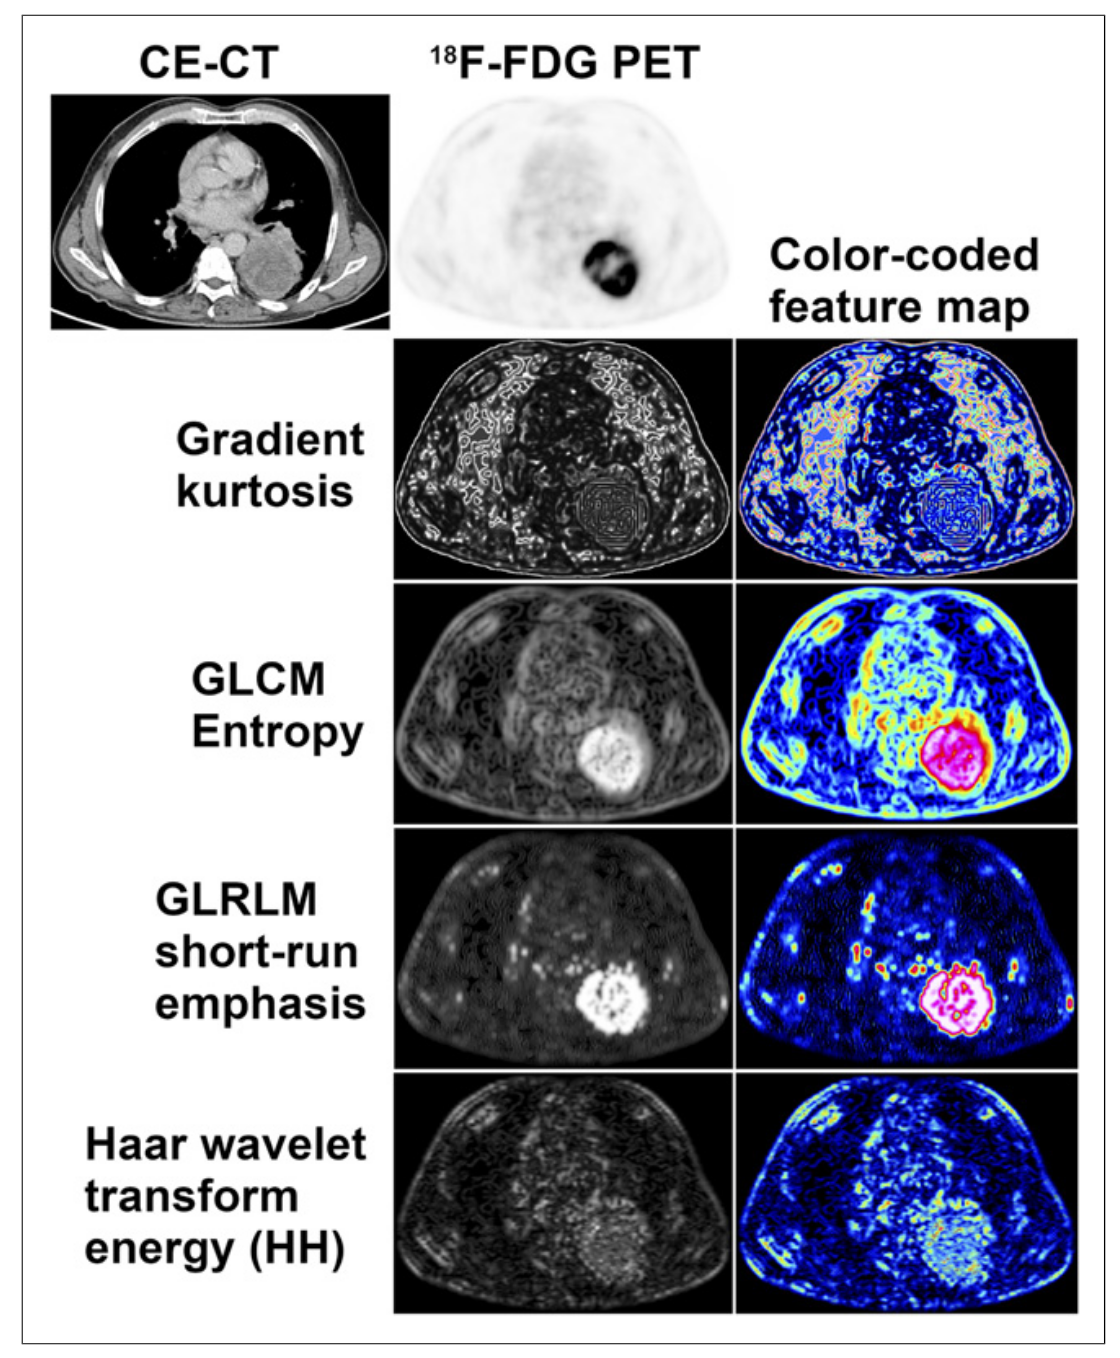
\includegraphics[width=0.6\textwidth]{figures/fig001.png}
    \caption*{Autor: \cite{mayerhoeferIntroductionRadiomics2020}}
    \label{fig:fig001}
\end{figure}

 A matriz de coocorrência de níveis de cinza, do termo \gls{glcm}, é um histograma em níveis de cinza de segunda ordem. O GLCM captura relações espaciais entre pares de \textit{pixels} ou \textit{voxels} com níveis de cinza pré-definidos, em diferentes direções (horizontal, vertical ou diagonal para análise 2D, 13 direções para 3D) e com uma distância pré-definida entre os \textit{pixels} ou \textit{voxels}. As características de GLCM incluem entropia, uma medida composta pela medida da inomogeneidade ou aleatoriedade dos níveis de cinza, momento angular de segunda ordem (também chamado de uniformidade ou energia), que reflete a homogeneidade ou ordem dos níveis de cinza e contraste, que enfatiza as diferenças nos níveis de cinza entre \textit{pixels} ou \textit{voxels} pertencentes a um par de \textit{pixel} ou \textit{voxel}. A Figura \ref{fig:fig002} ilustra um matriz que atua como um contador dos pares de \textit{pixel} ou \textit{voxel}.

 A matriz de comprimento de corrida de níveis de cinza, do termo 
 \textit{Gray-Level Run-length Matrix} (GLRLM), fornece informações sobre a distribuição espacial das sequências de \textit{pixels} consecutivos com os mesmos níveis de cinza, em uma ou mais direções, em 2 ou 3 dimensões. As características da GLRLM incluem fração, que avalia a porcentagem de \textit{pixels} ou \textit{voxels} dentro da região de interesse que fazem parte das sequências e, portanto, reflete a granulosidade. 

A matriz de zona do tamanho dos níveis de cinza, do termo \textit{Gray-Level Size Zone Matrix} (GLSZM), é baseada no mesmo princípio do GLRLM porém aqui, contagens do número de grupos (chamados zonas) de \textit{pixels} ou \textit{voxels} vizinhos interconectados com o mesmo nível de cinza formam a base para a matriz, como visto na Figura \ref{fig:fig002}. Uma textura mais homogênea resultará em uma matriz mais ampla e plana. A GLSZM não é calculada para diferentes direções, mas pode ser calculada para diferentes distâncias de \textit{pixels} ou \textit{voxels} que definem a vizinhança. As características da GLSZM podem ser calculadas em 2 dimensões (8 \textit{pixels} vizinhos) ou 3 dimensões (26 \textit{voxels} vizinhos) e, seguindo as definições da GLRLM, incluem fração (porcentagem de \textit{pixels} ou \textit{voxels} que fazem parte das zonas), ênfase em zonas pequenas e grandes, entre outras.

\begin{figure}[htbp]
    \centering
    \caption{Aplicação de Vizinhos em Abordagens Radiômicas}
    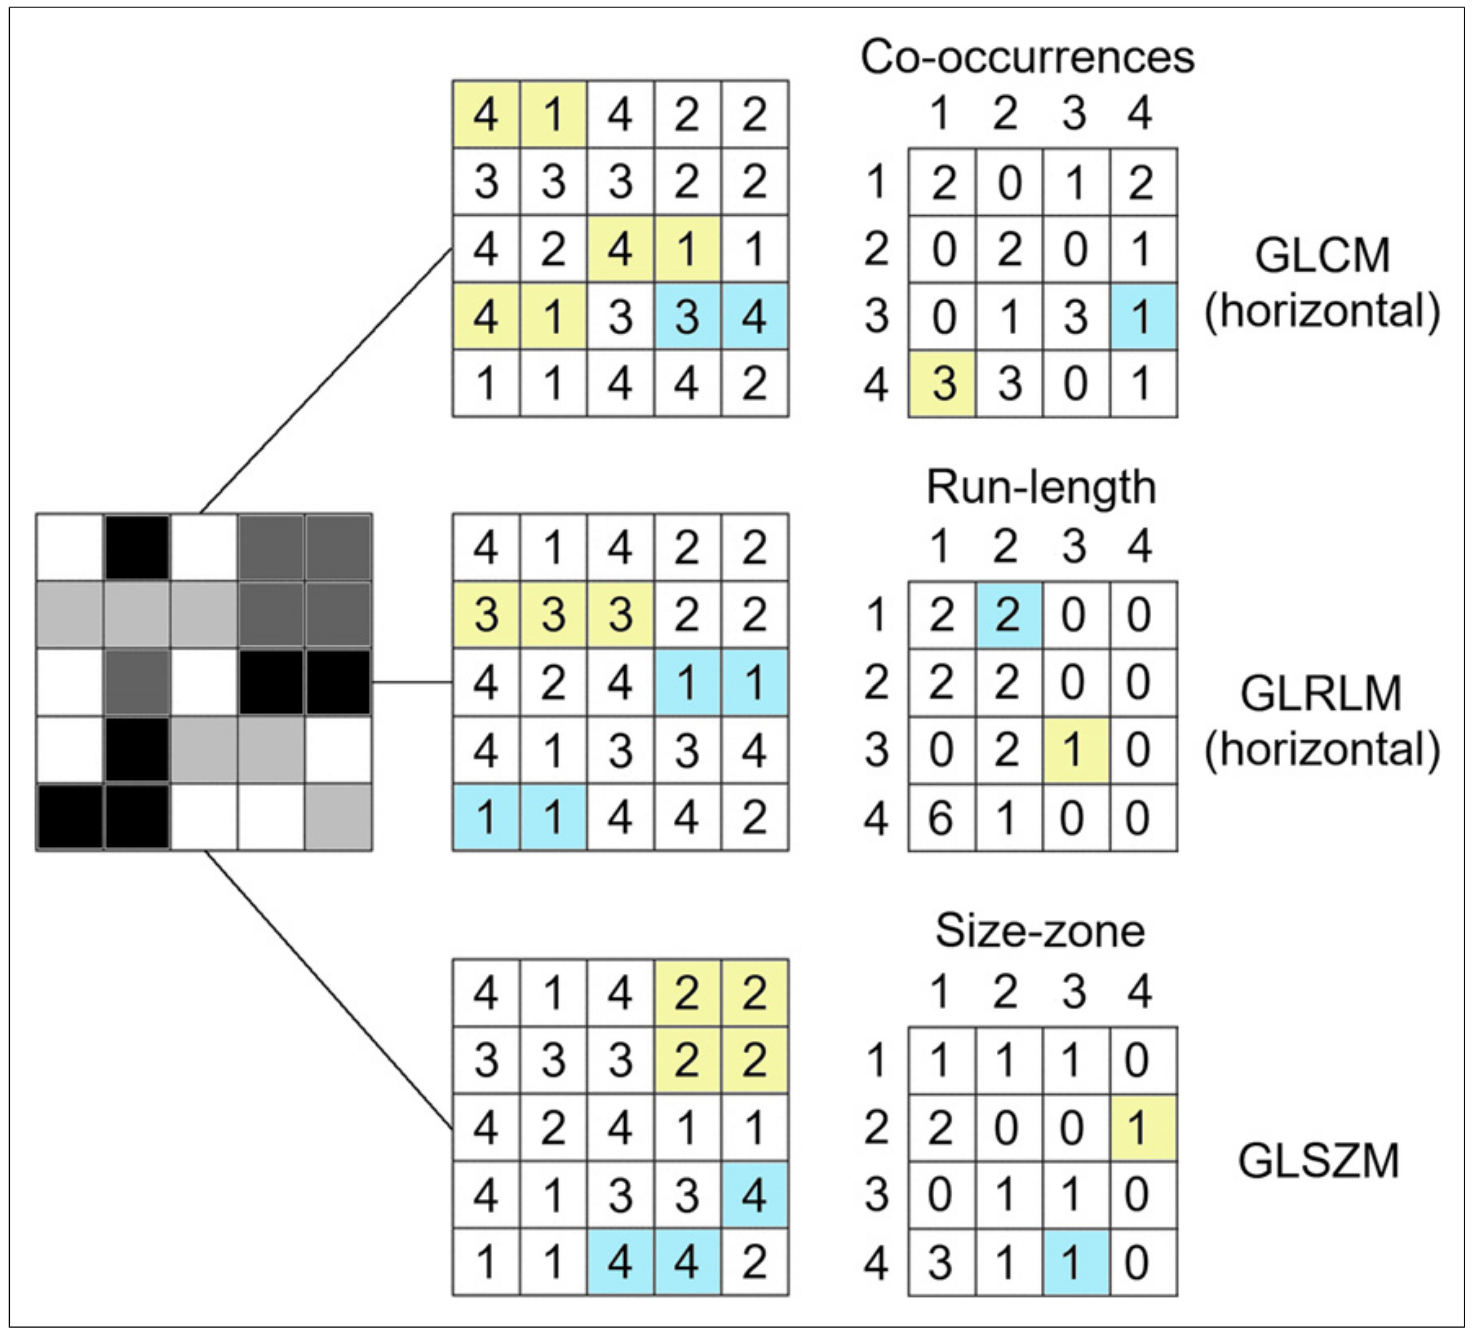
\includegraphics[width=0.6\textwidth]{figures/fig002.png}
    \caption*{Autor: \cite{mayerhoeferIntroductionRadiomics2020}}
    \label{fig:fig002}
\end{figure}

%--------------------------------------------------------
\subsection{Características de Modelo}

As análises baseadas em modelos visam interpretar características em níveis de cinza espaciais para caracterizar objetos ou formas. Um modelo parametrizado de geração de textura é calculado e ajustado à região de interesse, do termo \gls{roi}, e seus parâmetros estimados são utilizados como características radiômicas. O modelo autorregressivo é um exemplo de abordagem baseada em modelo e baseia-se na ideia de que o nível de cinza de um \textit{pixel} é uma soma ponderada dos níveis de cinza de 4 \textit{pixels} vizinhos. Além disso, o $\sigma$, o qual carrega informações sobre a variância do erro de previsão mínimo, mede a regularidade da textura. A análise fractal também produz recursos que podem ser usados na análise radiômica, em particular a dimensão fractal, que reflete a taxa de adição de detalhe estrutural com o aumento da magnificação, escala ou resolução e, portanto, serve como uma medida de complexidade. A lacunaridade, um recurso que mede a falta de invariância rotacional ou translacional, reflete a inomogeneidade \cite{mayerhoeferIntroductionRadiomics2020}.

%--------------------------------------------------------
\subsection{Características de Transformação}
Métodos baseados em transformadas, incluindo transformadas de \textit{Fourier}, \textit{Gabor} e de \textit{wavelets} de \textit{Haar}, analisam padrões de níveis de cinza em um espaço diferente. A transformada discreta \textit{wavelet} de \textit{Haar}, por exemplo, analisa o conteúdo da frequência de uma imagem em diferentes escalas. A decomposição por \textit{wavelets} de uma imagem é possível aplicando um par de filtros espelhados em quadratura, um filtro de passa-alta e um de passa-baixa. Embora o filtro de passa-alta destaque as mudanças no nível de cinza e, assim, enfatize detalhes da imagem, o filtro de passa-baixa suaviza a imagem em termos de nível de cinza, removendo detalhes da imagem. Após a decomposição do sinal, um conjunto de canais de frequência orientados espacialmente está disponível, o qual é usado para descrever a variabilidade local da imagem. As energias dentro dos canais de frequência são então usadas como características. A filtragem de passa-alta em ambas as direções, parte inferior da Figura \ref{fig:fig001}, captura detalhes diagonais, a filtragem de passa-alta seguida por filtragem de passa-baixa captura bordas verticais, a filtragem de passa-baixa seguida da filtragem de passa-alta captura bordas horizontais, e a filtragem de passa-baixa em ambas as direções captura as frequências mais baixas, em diferentes escalas. Notavelmente, a transformação por \textit{wavelets} pode ser usada não apenas para a geração de características radiômicas, mas também para segmentação de imagens ou como um passo de pré-processamento para análise de textura \cite{mayerhoeferIntroductionRadiomics2020}.

%---------------------------------------------------------
\section{REDES NEURAIS CONVOLUCIONAIS}
\label{sec:cnn}


Os autores \citeonline{lecunHandwrittenDigitRecognition1989} pesquisaram sobre o reconhecimento de caracteres em documentos escritos à mão, criando a arquitetura LeNet, uma rede que consiste em camadas convolucionais seguidas por camadas de \textit{pooling}, e finalizando com camadas totalmente conectadas. Os autores introduziram o \textit{backpropagation} a redes convolucionais, permitindo o aprendizado automático e substituindo o uso de técnicas para escolha manual de coeficientes. \citeonline{lecunHandwrittenDigitRecognition1989}, ainda estudando a classificação de caracteres, expandem a LeNet para a LeNet-5, uma rede que firmou a superioridade das redes convolucionais na tarefa de classificação de imagens se comparado a outros métodos da época.

Como o nome sugere, a camada convolucional desempenha um papel vital no funcionamento da \gls{cnn}. Os parâmetros das camadas concentram-se no uso de \textit{kernels} treináveis. Esses \textit{kernels} geralmente são pequenos em dimensionalidade espacial, mas se estendem por toda a profundidade da entrada. Quando os dados passam por uma camada convolucional, ela aplica cada filtro na dimensionalidade espacial da entrada para produzir um mapa de ativação 2D. À medida que se percorre a entrada, o produto escalar é calculado para cada valor nesse \textit{kernel}. A partir disso, a rede aprenderá \textit{kernels} que ``disparam'' quando detectam uma característica específica em uma determinada posição espacial da entrada. Esses são comumente conhecidos como ativações conforme descrito na Figura \ref{fig:fig024}.

\begin{figure}[h!]
    \centering
    \caption{Representação visual da camada convolucional. O elemento central do \textit{kernel} é aplica no vetor de entrada, que é calculado e substituído pela ponderada dele mesmo e de quaisquer pixels próximos.}
    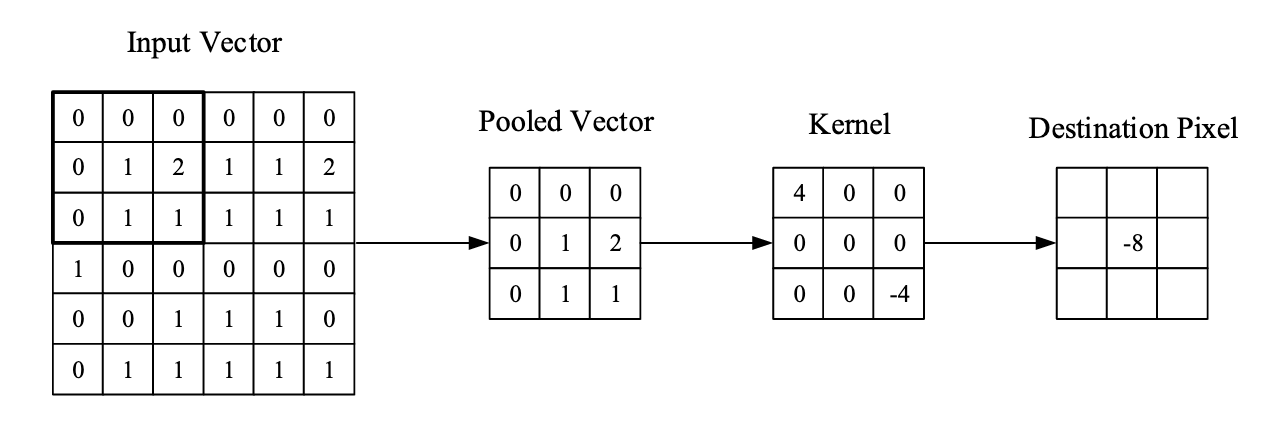
\includegraphics[width=0.6\textwidth]{figures/fig024.png}
    \caption*{Fonte: \cite{osheaIntroductionConvolutionalNeural2015c}}
    \label{fig:fig024}
\end{figure}

Cada \textit{kernel} terá um mapa de ativação correspondente, que será empilhado ao longo da dimensão de profundidade para formar o volume completo de saída da camada convolucional. Como mencionado anteriormente, treinar redes neurais artificiais tendo imagens como entrada resulta em modelos demasiadamente grandes para serem treinados de forma eficaz. Isso ocorre devido à conexão totalmente densa dos neurônios padrão das redes neurais artificiais. Para mitigar esse problema, cada neurônio em uma camada convolucional é conectado apenas a uma pequena região do volume de entrada \cite{osheaIntroductionConvolutionalNeural2015c}. 

A dimensionalidade dessa região é comumente chamada de ``tamanho do campo receptivo'' do neurônio. A magnitude da conectividade ao longo da profundidade geralmente é igual à profundidade da entrada. Por exemplo, se a entrada para a rede for uma imagem de tamanho 64x64x3 (uma imagem colorida RGB com dimensionalidade de 64x64) e for definido o tamanho do campo receptivo como 6x6, é obtido um total de 108 pesos em cada neurônio dentro da camada convolucional (6x6x3, onde 3 é a magnitude da conectividade na profundidade do volume). Para colocar isso em perspectiva, um neurônio padrão visto em outras formas de redes neurais artificiais conteria $12.288$ pesos cada. 

Camadas convolucionais também conseguem reduzir significativamente a complexidade do modelo por meio da otimização de sua saída. Essas otimizações são feitas por meio de três hiperparâmetros: profundidade, \textit{stride} e \textit{zero-padding}. 

A profundidade do volume de saída produzido pelas camadas convolucionais pode ser definida manualmente através do número de neurônios dentro da camada para uma mesma região da entrada. Isso pode ser observado em outras formas de redes neurais artificiais, onde todos os neurônios da camada oculta estão diretamente conectados a cada neurônio anterior. Reduzir esse hiperparâmetro pode minimizar significativamente o número total de neurônios da rede, mas também pode reduzir as capacidades de reconhecimento de padrões do modelo. 

Também é possível definir o \textit{stride}, que determina como é configurada a profundidade em torno da dimensionalidade espacial da entrada para posicionar o campo receptivo. Por exemplo, se o \textit{stride} for definido como 1, obtém-se um campo receptivo fortemente sobreposto, produzindo ativações extremamente grandes. Por outro lado, ao configurar o \textit{stride} para um número maior reduz a sobreposição e gera uma saída com dimensões espaciais menores.  

O \textit{zero-padding} é o processo de adicionar bordas à entrada, sendo um método eficaz para proporcionar maior controle sobre a dimensionalidade dos volumes de saída. É importante entender que, ao se usar dessas técnicas, a dimensionalidade espacial da saída das camadas convolucionais é alterada. Para este cálculo pode-se usar a seguinte Equação \ref{eq:cnn_output}.

\begin{equation}
\frac{(V - R) + 2Z}{S + 1}
\label{eq:cnn_output}
\end{equation}

O termo $V$ representa o tamanho do volume de entrada (altura x largura x profundidade), $R$ representa o tamanho do campo receptivo, $Z$ é a quantidade de \textit{zero-padding} definida e $S$ refere-se ao \textit{stride}. Se o resultado calculado a partir desta equação não for um número inteiro, o \textit{stride} foi configurado incorretamente, pois os neurônios não conseguirão se ajustar perfeitamente à entrada \cite{osheaIntroductionConvolutionalNeural2015c}.

%---------------------------------------------------------
\section{RESNET}
\label{sec:resnet}

A \textit{ResNet} (Rede Residual) é uma arquitetura de rede neural profunda amplamente utilizada em tarefas de visão computacional, como classificação de imagens, detecção de objetos e segmentação de imagens. Ela foi introduzida por \citeonline{heDeepResidualLearning2015}, e se destacou por ganhar a competição \textit{ImageNet} em 2015 com uma precisão significativamente maior do que as arquiteturas anteriores. A principal característica da \textit{ResNet} é sua capacidade de treinar redes muito profundas sem sofrer com o problema do ``desvanecimento do gradiente'' que afeta principalmente redes neurais profundas e impede o treinamento de progredir por conta de valores muito baixos de gradiente, problema este muito comum em redes tradicionais muito profundas. A \textit{ResNet} introduz um conceito chave chamado bloco residual que é um componente da rede onde a entrada do bloco é somada à sua saída antes de passar para a próxima camada. Esta conexão direta é chamada de conexão de salto e pode ser observada na Figura \ref{fig:fig013}.

\begin{figure}[h!]
    \centering
    \caption{Conexão de Salto}
    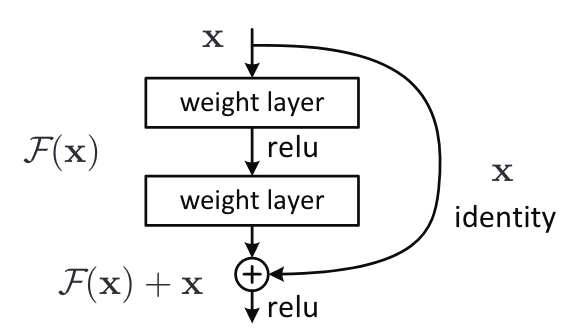
\includegraphics[width=0.6\textwidth]{figures/fig013.png}
    \caption*{Fonte: \cite{aiSelfAttentionBasedFusion2023}}
    \label{fig:fig013}
\end{figure}

A ResNet é composta por vários blocos residuais empilhados.
Existem várias versões da \textit{ResNet}, como \textit{ResNet}-18, \textit{ResNet}-34, \textit{ResNet}-50, \textit{ResNet}-101, e \textit{ResNet}-152, onde os números indicam a profundidade total da rede, ou seja, o número de camadas.

%--------------------------------------------------------
\subsection{Extração de Características Profundas}
\label{subsec:extract_features}

Para extrair características profundas das imagens de \gls{rmc}, foi empregada a arquitetura pré-treinada de uma rede \textit{ResNet50}. As redes \textit{ResNet50} ficaram muito conhecidas em meados do ano de 2015 por vencer diversas competições em visão computacional, incluindo o primeiro lugar na competição de classificação de imagens \textit{ILSVRC} 2015. As redes \textit{ResNet}, do termo \textit{Residual Networks}, inovaram em sua época trazendo uma nova forma de treinar modelos que possuem maior profundidade, chegando a mais de 100 camadas, com resultados superiores à outros modelos convolucionais competitivos, como o \textit{VGG19}, sem sofrer sintomas comuns a redes neurais muito profundas como o \textit{overfitting} e a saturação ou a ausência dos gradientes em tempo de treino. Os autores da \textit{ResNet} sugeriram o uso de saltos de conexão entre as camadas da rede afim de manter os gradientes relevantes e controlados entre uma camada e outra.  A \textit{ResNet50} é um modelo de rede neural convolucional profunda de $50$ camadas que compreende muitos blocos residuais. A cada bloco, se encontram módulos de convolução e uma conexão de salto que transfere a informação do bloco anterior para o próximo bloco. A conexão de salto ajuda a reter a informação semântica mais baixa aprendida nas camadas anteriores, que de outra forma se tornaria abstrata devido à conexão de longa cadeia. A conexão de salto também evita que o gradiente desapareça nas camadas mais profundas, fornecendo um caminho alternativo para a retropropagação. A informação da conexão de salto é adicionada à informação calculada em cada bloco \cite{heDeepResidualLearning2015}.

Várias abordagens de sucesso aplicaram redes convolucionais para extrair características genéricas para tarefas de recuperação de imagens e obtiveram resultados promissores. Elas utilizam principalmente o poder das características locais para gerar uma representação de uma imagem genérica baseada em redes convolucionais pré-treinadas. As representações das camadas finais da rede convolucional são utilizadas para capturar características semânticas para o fim de nível de categoria à classificação que o modelo se dispõe \cite{alzubiContentbasedImageRetrieval2017b}.

%---------------------------------------------------------
\section{REDE SQUEEZE AND EXCITATION}
\label{sec:se_net}

Para cada camada convolucional, um conjunto de filtros é aprendido para expressar padrões de conectividade espacial local ao longo dos canais de entrada. Em outras palavras, espera-se que os filtros convolucionais sejam combinações informativas ao fundir informações espaciais e baseadas nos canais dentro de campos receptivos locais.
Ao empilhar uma série de camadas convolucionais intercaladas com não linearidades e redução de amostragem, as \gls{cnn}s são capazes de capturar padrões hierárquicos com campos receptivos globais, funcionando como descrições de imagem poderosas \cite{huSqueezeandExcitationNetworks2018}. 

Estudos de \citeonline{huSqueezeandExcitationNetworks2018}, demonstraram que o desempenho das redes pode ser aprimorado ao incorporar explicitamente mecanismos de aprendizado que ajudam a capturar correlações espaciais, sem a necessidade de supervisão adicional. Neste sentido, foi proposto um mecanismo que permite à rede realizar a recalibração de características, por meio do qual ela pode aprender a usar informações globais para enfatizar seletivamente características informativas e suprimir aquelas menos úteis. Este estudo intitulado \gls{se} Net, investiga um aspecto diferente no design arquitetural, a relação entre canais ao introduzir o bloco \gls{se}.

Os blocos \gls{se} podem ser construídos para qualquer transformação conforme a indica a Equação \ref{eq:se_transform} onde $\mathbf{U}$ representa a saída da transformação inicial da rede neural, antes da aplicação do bloco \gls{se}.

\begin{equation}
\mathcal{F}_{tr} : \mathbf{X} \rightarrow \mathbf{U}, \mathbf{X} \in R^{H' \times W' \times C'}, \mathbf{U} \in R^{H \times W \times C}
\label{eq:se_transform}
\end{equation}

Sendo $\mathbf{V} = [\mathbf{v}_1, \mathbf{v}_2, \ldots, \mathbf{v}_C]$ os filtros de aprendidos onde $\mathbf{v}_C$ se refere ao parâmetro de $c$-ésimo filtro. As saídas das convoluções podem ser escritas da seguinte forma: $\mathcal{F}_{tr} \mathbf{U} = [\mathbf{u}_1, \mathbf{u}_2, \ldots, \mathbf{u}_C]$, sendo o termo $\mathbf{u}_C$ descrito na equação \ref{eq:se}. 

\begin{equation}
\mathbf{u}_c = \mathbf{v}_c \ast \mathbf{X} = \sum_{s=1}^{C'} \mathbf{v}_c^s \ast \mathbf{x}^s
\label{eq:se}
\end{equation}

O termo $\ast$ denota convolução, $\mathbf{v}_c$ é um filtro espacial 2D e representa um único canal de $\mathbf{v}_c$ que atua no canal correspondente de $\mathbf{X}$. 
Tendo como o objeto garantir que a rede seja capaz de aumentar sua sensibilidade a características informativas, para que possam ser exploradas por transformações subsequentes, e suprimir as menos úteis. Foi proposto um modelo explícito das interdependências de canal para recalibrar as respostas dos filtros em duas etapas — \textit{squeeze} e \textit{excitation} —, antes de serem alimentadas na transformação subsequente. Um diagrama de um bloco de construção \gls{se} é demonstrado na Figura \ref{fig:fig025}.

\begin{figure}[h!]
    \caption{Fluxo do Bloco SE - Após blocos convolucionais normais, uma cama da de \textit{squeeze} seguida e uma camada de \textit{excitation} é aplicada e por fim os valores originais são escalonados pelo resultado.}
    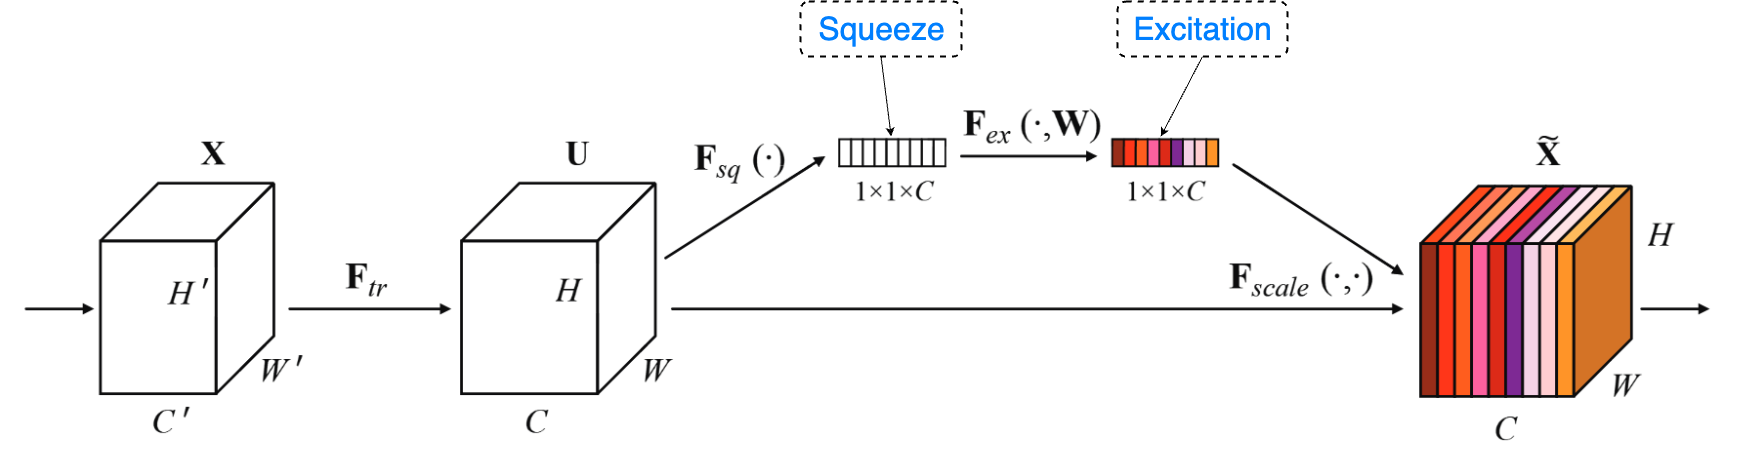
\includegraphics[height=0.27\textwidth]{figures/fig025.png}
    \caption*{Fonte: Adaptado de \cite{huSqueezeandExcitationNetworks2018}}
    \label{fig:fig025}
\end{figure}


%---------------------------------------------------------
\subsection{Squeeze: Informação Global}
\label{subsec:squeeze}

Para lidar com o problema de explorar as dependências entre os canais, é considerado o primeiro sinal de cada canal nas características de saída. Cada um dos filtros aprendidos opera com um campo receptivo local e, consequentemente, cada unidade da saída da transformação $\mathbf{U}$ é incapaz de explorar informações contextuais fora dessa região. Esse problema se torna ainda mais grave nas camadas mais baixas da rede, cujos campos receptivos são menores.

Para mitigar esse problema, foi proposto comprimir as informações espaciais globais em um descritor de canal. Isso é obtido por meio de uma instrução de \textit{average pooling} global para gerar estatísticas específicas de cada canal. O cálculo do \textit{average pooling} pode ser conferido na Equação \ref{eq:avgpool}.

\begin{equation}
z_c = \mathbf{F}_{sq}(\mathbf{u}_c) = \frac{1}{H \times W} \sum_{i=1}^{H} \sum_{j=1}^{W} u_c(i, j)
\label{eq:avgpool}
\end{equation}

%---------------------------------------------------------
\subsection{Excitation: Recalibração Adaptativa}
\label{subsec:excitation}

Para aproveitar as informações agregadas na operação de \textit{squeeze}, uma segunda operação que tem como objetivo capturar completamente as dependências entre os canais. Para cumprir esse objetivo, a função deve atender a dois critérios: primeiro, ela precisa ser flexível (em particular, deve ser capaz de aprender uma interação não linear entre os canais) e, segundo, ela deve aprender uma relação não mutuamente exclusiva, pois é de interesse garantir que vários canais possam ser enfatizados, em vez de apenas uma ativação \textit{one-hot}. Para atender a esses critérios, emprega-se um mecanismo de \textit{gating} simples com uma ativação sigmoide conforme demonstrado na Equação \ref{eq:excitation}:

\begin{equation}
\mathbf{s} = \mathbf{F}_{ex}(\mathbf{z}, \mathbf{W}) = \sigma(g(\mathbf{z}, \mathbf{W})) = \sigma(\mathbf{W}_2 \delta(\mathbf{W}_1 \mathbf{z}))
\label{eq:excitation}
\end{equation}

\noindent sendo que o termo $\delta$ se refere à função de ativação ReLU \cite{nairRectifiedLinearUnits}, $W_1 \in \mathbb{R}^{\frac{C}{r} \times C}$ e $W_2 \in \mathbb{R}^{C \times \frac{C}{r}}$. Para limitar a complexidade do modelo e auxiliar na generalização, o mecanismo de \textit{gating} é parametrizado formando um gargalo com duas camadas totalmente conectadas ao redor da não linearidade, ou seja, uma camada de redução de dimensionalidade com os parâmetros $W_1$ e razão de redução $r$, seguida de uma ReLU e, em seguida, uma camada de aumento de dimensionalidade com os parâmetros $W_2$. A saída final do bloco é obtida ao redimensionar a saída da transformação $U$ com as ativações conforme Equação \ref{eq:se_scale}.

\begin{equation}
\tilde{\mathbf{x}}_c = \mathbf{F}_{scale}(\mathbf{u}_c, s_c) = s_c \cdot \mathbf{u}_c 
\label{eq:se_scale}
\end{equation}

\noindent onde $\tilde{\mathbf{X}} = [\tilde{\mathbf{x}}_1, \tilde{\mathbf{x}}_2, \dots, \tilde{\mathbf{x}}_C]$ e $\mathbf{F}_{scale}(\mathbf{u}_c, s_c)$ se referem a multiplicação no nível dos canais entre os mapas de características $\mathbf{u}_c \in \mathbb{R}^{H \times W}$ e o valor escalar $s_c$.

%---------------------------------------------------------
\subsection{Utilização em redes conhecidas: SE-Resnet}
\label{subsec:util_resnet}

A flexibilidade do bloco \gls{se} significa que ele pode ser aplicado diretamente a transformações além das convoluções padrão. Para ilustrar esse ponto, os autores desenvolveram as redes \gls{se}  integrando blocos \gls{se} em arquiteturas modernas com \textit{designs} sofisticados. A Figura \ref{fig:fig026} demonstra o esquema de um módulo SE-ResNet. Nele, a transformação do bloco \gls{se}, $F_{tr}$, é considerada o ramo não identidade de um módulo residual. As operações de \textit{squeeze} e \textit{excitation} atuam antes da soma com o ramo identidade.


\begin{figure}[h!]
    \centering
    \caption{Módulo SE-Resnet}
    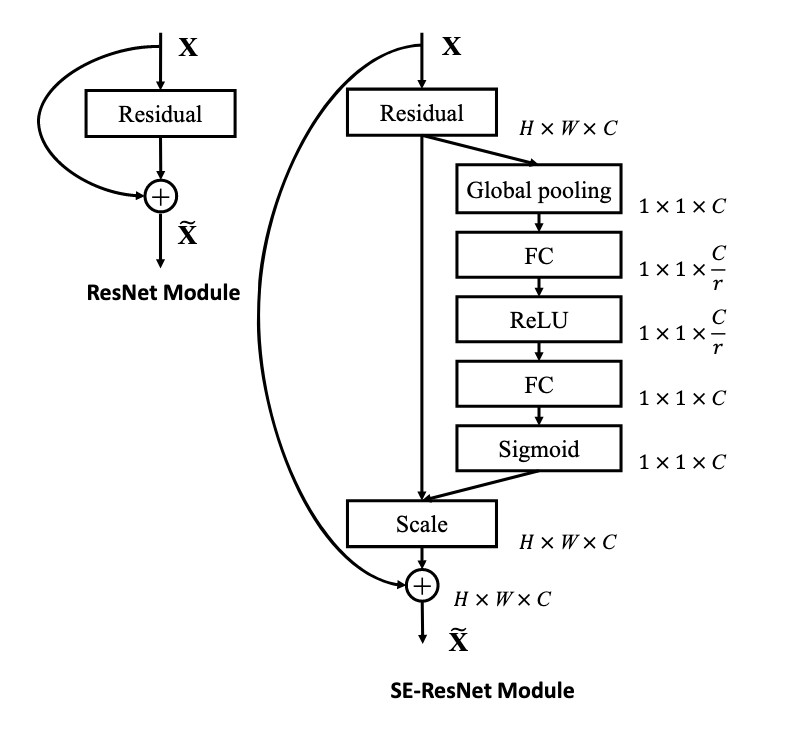
\includegraphics[width=0.6\textwidth]{figures/fig026.png}
    \caption*{Fonte: Adaptado de \cite{huSqueezeandExcitationNetworks2018}}
    \label{fig:fig026}
\end{figure}

Para que o bloco SE proposto seja viável na prática, ele deve fornecer um equilíbrio eficaz entre a complexidade do modelo e o desempenho, o que é importante para escalabilidade. Foi definida uma razão de redução $r$ como 16 em todos os experimentos, exceto onde indicado de outra forma. 

O valor $r$ é um hiperparâmetro importante pois permite variar a capacidade e o custo computacional dos blocos \gls{se} no modelo. O autor do trabalho conduz experimentos baseados no SE-ResNet-50 para uma variedade de valores diferentes de $r$. A comparação vista na Figura  \ref{fig:fig027}, revela que o desempenho não melhora monotonicamente com o aumento da capacidade. Isso provavelmente é resultado do bloco SE ajustar em excesso as interdependências de canal do conjunto de treinamento. Definir $r = 16$ alcançou um bom equilíbrio entre precisão e complexidade e, consequentemente, foi o valor utilizado pelos autores nos experimentos. O Algoritmo \ref{alg:se_block} reflete a implementação do bloco \gls{se}.

\begin{figure}[h!]
    \centering
    \caption{Conjunto de Validação Aplicado na SE-ResNet-50}
    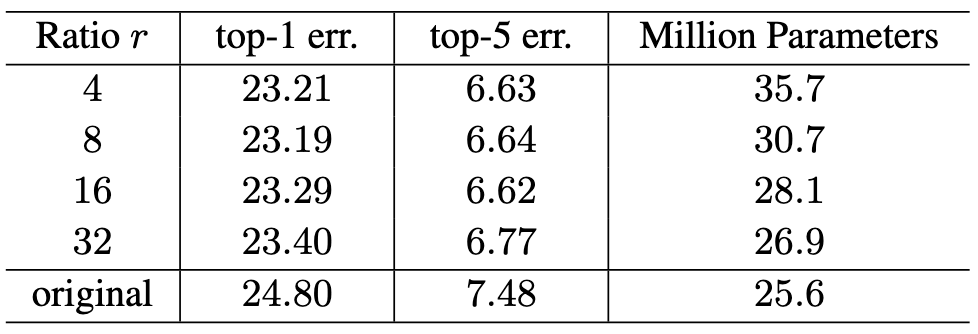
\includegraphics[width=0.6\textwidth]{figures/fig027.png}
    \caption*{Fonte: Adaptado de \cite{huSqueezeandExcitationNetworks2018}}
    \label{fig:fig027}
\end{figure}

% ----------------- ALGORITMO SQUEEZE AND EXCITATION NET ------------------
\begin{algorithm}
\caption{Bloco Squeeze-and-Excitation (SE)}
\label{alg:se_block}
\textbf{Entrada:} Mapa de características $\mathbf{U} \in \mathbb{R}^{H \times W \times C}$\\
\textbf{Saída:} Mapa de características recalibrado $\tilde{\mathbf{U}} \in \mathbb{R}^{H \times W \times C}$
\begin{algorithmic}[1]
\STATE \textbf{Squeeze:} Executa o \textit{average pooling} global para agregar as dimensões espaciais:
\[
z_c = \frac{1}{H \times W} \sum_{i=1}^H \sum_{j=1}^W u_c(i, j), \quad \forall c \in \{1, \dots, C\}
\]
\STATE \textbf{Excitation:} Usa duas camadas totalmente conectadas para modelar a interdependência dos canais:
\[
\mathbf{s} = \sigma(\mathbf{W}_2 \delta(\mathbf{W}_1 \mathbf{z}))
\]
onde:
\begin{itemize}
    \item $\mathbf{W}_1 \in \mathbb{R}^{\frac{C}{r} \times C}$: Camada de redução de dimensionalidade
    \item $\mathbf{W}_2 \in \mathbb{R}^{C \times \frac{C}{r}}$: Camada de restauração da dimensão original
    \item $\delta$: Ativação ReLU
    \item $\sigma$: Ativação Sigmoide
\end{itemize}
\STATE \textbf{Reescala:} Recalibra o mapa de características usando as ativações:
\[
\tilde{\mathbf{u}}_c = s_c \cdot \mathbf{u}_c, \quad \forall c \in \{1, \dots, C\}
\]
\RETURN $\tilde{\mathbf{U}} = [\tilde{\mathbf{u}}_1, \tilde{\mathbf{u}}_2, \dots, \tilde{\mathbf{u}}_C]$
\end{algorithmic}
% \caption*{Fonte: Autor}
\end{algorithm}


%--------------------------------------------------------
\section{ARQUITETURA TRANSFORMERS}
\label{sec:transformers}

Os \textit{transformers} consistem em uma arquitetura que possui como um de seus propósitos resolver as limitações das arquiteturas recorrentes e sua dificuldade em manter as relações entre pontos dentre as camadas recorrentes além das restrições vinculadas ao custo de computação sequencial. O modelo de arquitetura \textit{transformers} se utiliza do mecanismo de atenção e este se tornou parte essencial de modelos eficazes de modelagem e transdução de sequências em diversas tarefas, permitindo a modelagem de dependências sem considerar a distância entre elas nas sequências de entrada ou saída. Os \textit{transformers} como arquitetura descarta o uso de módulos de recorrência e se utiliza inteiramente do mecanismo de atenção para capturar as dependências globais entre entrada e saída. Os \textit{transformers} também são responsáveis por um ganho significante em paralelismo em sua execução \cite{vaswaniAttentionAllYou2023}.

\begin{figure}[htbp]
    \centering
    \caption{Arquitetura \textit{Transformers}}
    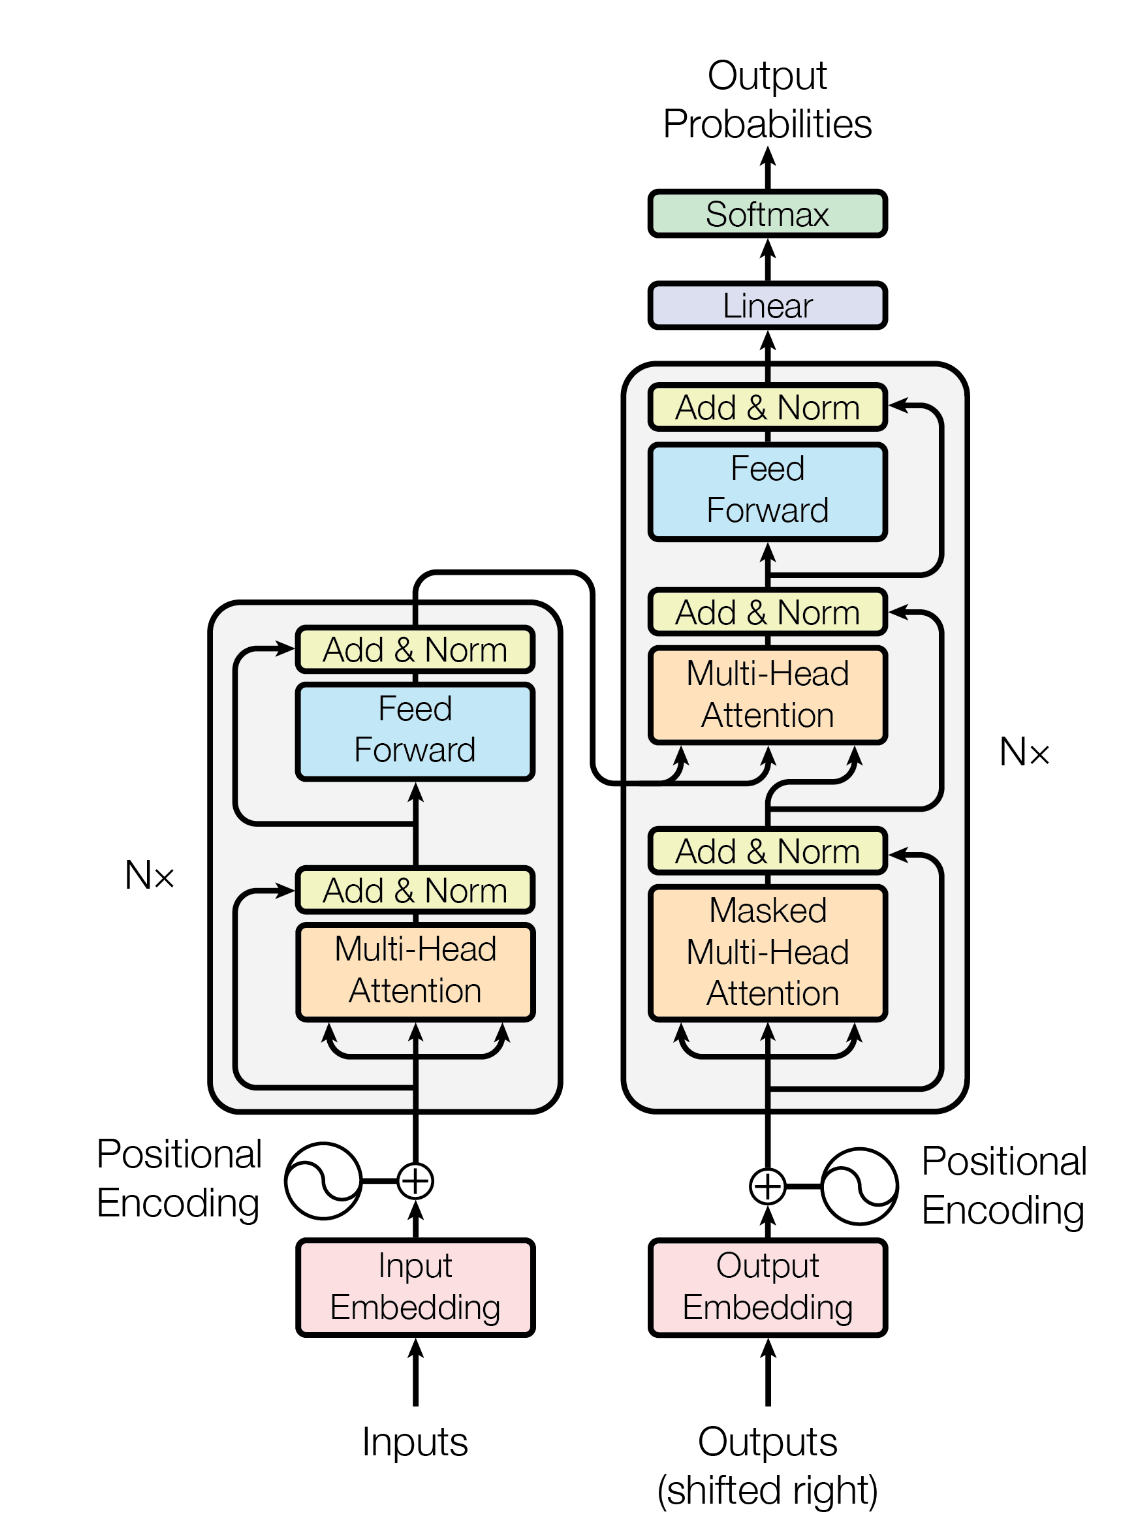
\includegraphics[scale=0.6]{figures/fig004.png}
    \caption*{Autor: \citeonline{vaswaniAttentionAllYou2023}}
    \label{fig:fig004}
\end{figure}

Os \textit{transformers} são compostos por um \textit{Encoder} e um \textit{Decoder}, representados pelos os blocos da esquerda e direita respectivamente apresentados na Figura \ref{fig:fig004}. Em ambos \textit{Encoder} e \textit{Decoder}, tem-se como bloco cerne da rede intitulado de atenção multi-cabeças. O mecanismo de atenção pode ser descrito mapeando uma \textit{query} a um par de chave e valor, onde a \textit{query}, a chave e o valor são todos vetores de saída. A saída é computada como uma soma ponderada dos valores onde o peso destinado a cada valor é computado por uma função de compatibilidade da \textit{query} com a chave correspondente.

\begin{figure}[htbp]
    \centering
    \caption{Módulo de Atenção Multi-Cabeças}
    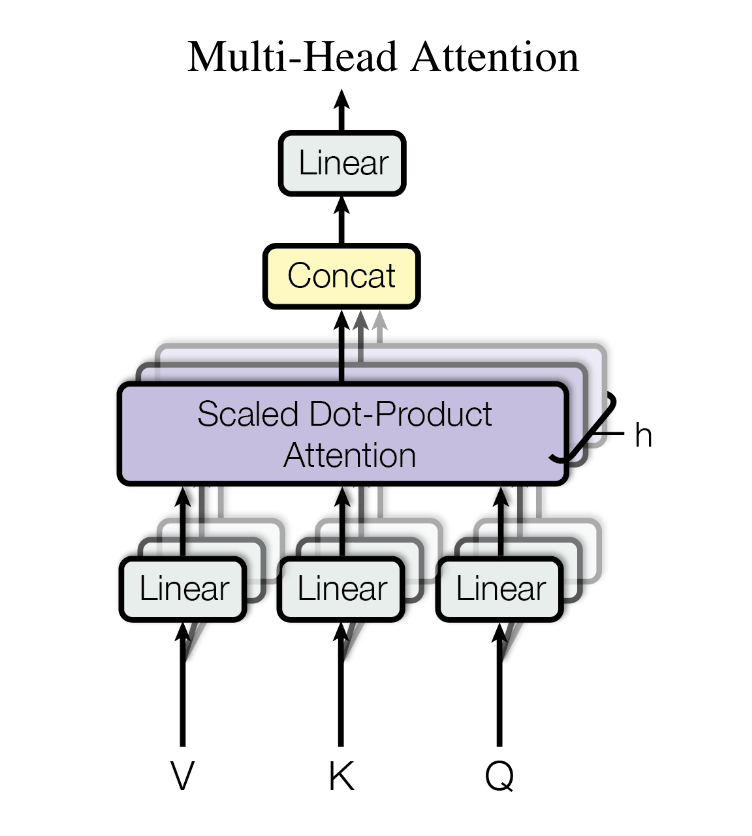
\includegraphics[width=0.6\textwidth]{figures/fig005.png}
    \caption*{Autor:\cite{vaswaniAttentionAllYou2023}}
    \label{fig:fig005}
\end{figure}

O mecanismo de atenção é particularmente chamado de ``Atenção de Produto Escalar Dimensionado'', visto na Figura \ref{fig:fig005}. A entrada consiste em \textit{queries} e chaves de dimensão $d_{k}$ e valores de dimensão $d_{v}$. São calculados os produtos escalares da consulta com todas as chaves e dividido por $\sqrt{d_{k}}$, para fins de controle dos valores em uma menor amplitude. Em seguida, aplica-se uma função \textit{softmax} para obter as probabilidades sobre os valores. Na prática, é calculada a função de atenção em um conjunto de consultas simultaneamente, agrupadas em uma matriz $Q$. As chaves e os valores também são agrupados em matrizes $K$ e $V$. Calcula-se a matriz de saídas como:

\begin{equation}
\text{Attention}(Q, K, V) = \text{softmax}\left(\frac{QK^T}{\sqrt{d_k}}\right)V
\label{eq:attention}
\end{equation}

Dentre os pontos de vantagem do mecanismo de atenção, se destacam: o total de poder computacional por camada, o total de computação que pode ser paralelizada e o poder de capturar a relação de dependência entre dados que se encontram distantes espacialmente um do outro. Como benefício adicional, o mecanismo de atenção pode gerar modelos mais interpretáveis, sob o ponto de vista de como os \textit{tokens} se correlacionam. Não apenas as cabeças de atenção individuais claramente aprendem a executar diferentes tarefas, muitas parecem exibir comportamentos relacionados à estrutura sintática e semântica das frases, no caso da aplicação em \textit{tokens} oriundos de textos.

%--------------------------------------------------------
\section{OTIMIZADOR ADAM}
\label{sec:adam}

Toda rede neural é treinada aplicando otimização em uma determinada função objetivo afim de minimizar o erro perante os dados de treinamento. Neste contexto, o presente trabalho escolhe o \gls{adam} como otimizador dada sua adaptatividade.

O método \gls{adam}, introduzido por \citeonline{kingmaAdamMethodStochastic2014}, é um método popular para o treinamento de modelos de \gls{ap}. O \gls{adam} combina os benefícios de outras duas técnicas de otimização, o \textit{AdaGrad} e o \textit{RMSProp}. O \gls{adam} é um método de otimização estocástica eficiente que requer apenas gradientes de primeira ordem com pouca exigência de memória. O método calcula taxas de aprendizado adaptativas individuais para diferentes parâmetros a partir de estimativas dos primeiros e segundos momentos dos gradientes.

Algumas das vantagens do \gls{adam} podem ser elencadas: taxas de aprendizado adaptativas, que levam a uma convergência mais rápida e eficiente se comparadas com métodos de aprendizado fixos; robustez, que suportam gradientes esparsos de forma efetiva, cruciais para diversas aplicações de \gls{ap} atuais; fácil de utilizar, pois requer menos ajustes de parâmetros a tornando amigável ao usuário e acessível a uma grande gama de tarefas.

\chapter{Trabalhos Relacionados}
\label{chap:trabalhos_relacionados}
\vspace{-\baselineskip} %Manter para garantir o espaçamento da biblioteca.

Aplicar a unificação de técnicas radiômicas e aprendizado profundo na pesquisa de cardiomiopatia tem recebido cada vez mais atenção da comunidade científica.
Neste capítulo serão apresentados trabalhos e metodologias correlatos ao esforço de outros autores a cerca deste tema. Será descrito como foi a metodologia utilizada na revisão sistemática da literatura \cite{petersenGuidelinesConductingSystematic2015a}, assim como trabalhos que trazem ideias próximas ao proposto neste trabalho.

%---------------------------------------------------------
\section{REVISÃO SISTEMÁTICA DA LITERATURA} 
\label{sec:rev_sistematica}

Para a fase exploratória dos trabalhos relacionados, foi utilizada a ferramenta \textit{Parsifal} \footnote{https://parsif.al} com o objetivo de identificar estudos que aplicam a análise radiômica no contexto de cardiomiopatia. O objetivo inicialmente definido foi o seguinte: ``Identificar estudos onde se aplica análise radiômica a cardiopatia. Como segunda opção, alguma outra doença de natureza cardíaca''. A pesquisa teve como objetivo responder as seguintes perguntas: quais desafios descritos nos estudos prévios e se há replicabilidade da proposta no contexto de cardiomiopatia. As palavras chaves selecionadas foram: \textit{cardiac}, \textit{cardiomyopathy} e \textit{radiomics}. A palavra de busca selecionada foi: ``\textit{radiomics} AND "data extraction" AND (\textit{cardiac} OR \textit{cardiomyopathy})'' e a última atualização das pesquisas foram feitas em agosto de 2023. Os resultado do filtro de busca são apresentados na Tabela \ref{tab:resultado_busca}. 
\newline

\begin{table}[hbtp]
    \caption{Resultados dos Artigos}
    \centering
    \renewcommand{\arraystretch}{1.4} % default é 1 
    \begin{tabular}{|c|c|}
    \hline 
          \textbf{Origem} & \textbf{Artigos}  \\ 
    \hline 
        IEEE & 6 \\ 
        PUBMED & 19 \\ 
        Science@Direct & 24 \\ 
    \hline 
    \end{tabular} 
    \caption*{Fonte: Autor}
    \label{tab:resultado_busca}
\end{table}

A partir dos resultados foram aplicados os critérios de inclusão e exclusão conforme descritos na Tabela \ref{tab:criterios}.

\begin{table}[hbtp]
    \centering
    \caption{Critérios de Inclusão e Exclusão}
    \renewcommand{\arraystretch}{1.4} % default é 1 
    \begin{tabular}{|l|l|}
    \hline 
          \multicolumn{1}{|c|}{\textbf{Critério de Inclusão}} & \multicolumn{1}{c|}{\textbf{Critério de Exclusão}}  \\ 
    \hline 
        \quad Contém ressonância magnética? & \quad Estudos Duplicados   \\ 
        \quad O objeto de estudo é o coração? & \quad Estudos Secundários ou Terciários \\
        \quad Usa análise de textura? & \quad Estudos que não estão em PT ou EN\\
        \quad Utiliza análise radiômica? & \quad Leitura cinza  \\
        \quad É cardiomiopatia? & \quad Não aplica técnicas computacionais\\
        & \quad Não trata do coração \\
        & \quad Não usa RM \\
        & \quad Trabalho que atua somente com dados genômicos \\ 
    \hline 
    \end{tabular} 
    \caption*{Fonte: Autor}
    \label{tab:criterios}
\end{table}

Critérios de inclusão também foram aplicados e são apresentados na Tabela \ref{tab:questoes}. Dentre estes critérios, cada artigo é representado pela soma das pontuações obtidas pelos critérios e os artigos que obtiveram uma nota menor que 3 foram excluídos da revisão. Para as notas, ficou definido como pontuação: $1$ para critério aceito, $0,5$ para critério parcialmente aceito e $0$ para critério não atingido. Uma vez aplicado os critérios e filtrado mediante pontuação, restaram $18$ dos $49$ artigos iniciais. Para fins de elucidar, o critério de mais de dois autores envolvem colaboração entre diferentes especialistas ou instituições, seguindo por vezes, padrões mais rigorosos e tendo maior visibilidade na comunidade científica.


\begin{table}[hbtp]
    \centering
    \caption{Questões de Aceitação}
    \renewcommand{\arraystretch}{1.4} % default é 1 
    \begin{tabular}{|l|}
    \hline 
          \multicolumn{1}{|c|}{\textbf{Questões}} \\ 
    \hline 
        \quad É descrita as limitações do estudo? \\
        \quad Há um experimento bem descrito para avaliar a proposta? \\
        \quad Há mais de 2 autores? \\
        \quad O trabalho apresenta resultados? \\
        \quad A introdução apresenta o problema de forma clara \\
        \quad É análise sistemática da literatura? \\
    \hline 
    \end{tabular} 
    \caption*{Fonte: Autor}
    \label{tab:questoes}
\end{table}

O diagrama com o funil de seleção aplicado é apresentado na Figura \ref{fig:fig021}. É possível verificar na imagem, por exemplo, que foram removidos $28$ artigos dos $49$ artigos selecionados inicialmente, restando $21$. Aplicando os critérios de qualidade, foram selecionados $18$ artigos. Dentre os artigos selecionados, $3$ foram excluídos por não agregarem o suficiente ou por serem redundantes.

\begin{figure}[H]
    \centering
    \captionsetup{width=0.98\textwidth, justification=justified}
    \caption{Funil da Seleção da Literatura - Etapas do processo de busca, filtragem e seleção de artigos com base em critérios de inclusão, exclusão e qualidade, resultando no conjunto final de estudos analisados.}
    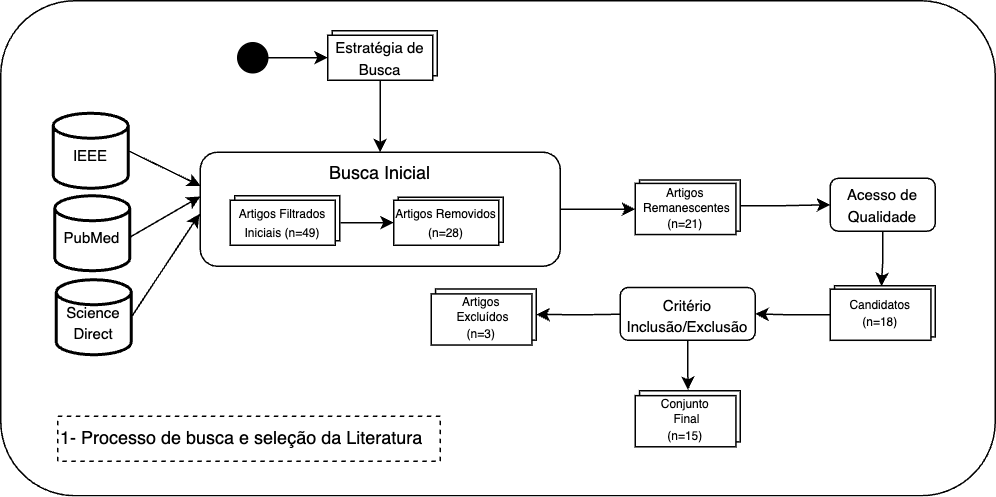
\includegraphics[scale=0.47]{figures/fig021.png}
    \caption*{Fonte: Autor}
    \label{fig:fig021}
\end{figure}

%---------------------------------------------------------
\section{ANÁLISE RADIÔMICA COM ATENÇÃO}
\label{sec:analise_radiomica_com_atencao}

\citeonline{jiangMRIBasedRadiomics2021} conduziram um estudo abrangente que aproveita as capacidades do aprendizado de máquina para melhorar os processos diagnósticos em oncologia, especificamente focando no câncer de colo de útero em estágio inicial. Sua pesquisa, intitulada ``Abordagem Radiômica Baseada em Ressonância Magnética com Aprendizado Profundo para Predição de Invasão Vascular em Câncer de Colo de Útero em Estágio Inicial'', foca na aplicação de técnicas de aprendizado profundo em dados de \gls{rmc} multiparamétrica para prever a invasão vascular, um fator crítico para determinar a agressividade do câncer de colo de útero e informar estratégias de tratamento.

O estudo utilizou um conjunto substancial de dados compreendendo $1.070$ imagens de ressonância magnética com contraste dinâmico T1 (DCE-T1) e $986$ imagens de ressonância magnética ponderadas em T2 (T2WI) e coletadas de $167$ pacientes diagnosticadas com câncer do colo do útero em estágio inicial entre janeiro de $2014$ e agosto de $2018$. Os pesquisadores empregaram uma nova estrutura de aprendizado profundo que integrou esses dois tipos distintos de varreduras em imagens de \gls{rmc} para criar um modelo preditivo robusto. Implementando uma estratégia de aprendizado em conjunto com atenção, o modelo efetivamente distinguiu entre casos com invasão vascular e aqueles sem. Quatro modelos de CNN foram utilizados: VGGNet, GoogLeNet (Inception-v3), Residual Network (ResNet) e \textit{DenseNet}. Um módulo padrão de \gls{se}  e o módulo de atenção de bloco convolucional, do termo inglês \gls{cbam},  foram introduzidos após cada bloco de convolução da rede \textit{AdaptedVGG19} para fornecer um \textit{AdaptedVGG19-SE} e um \textit{AdaptedVGG19-CBAM}, respectivamente. A arquitetura proposta é vista na Figura \ref{fig:fig007}.

O desempenho preditivo dos modelos foi rigorosamente avaliado, com os modelos finais alcançando uma \gls{auc} de 0,911. Essa alta \gls{auc} indica uma forte capacidade do modelo para classificar corretamente a presença ou ausência de invasão vascular, com métricas de sensibilidade e especificidade também demonstrando precisão diagnóstica substancial.

Esta pesquisa demonstra o potencial de integrar algoritmos de aprendizado profundo com dados de imagem complexos para melhorar as avaliações diagnósticas pré-operatórias. Os achados de \citeonline{jiangMRIBasedRadiomics2021} sugerem que tais abordagens analíticas avançadas podem fornecer suporte substancial na tomada de decisões clínicas, potencialmente levando a planos de tratamento mais personalizados e melhores resultados para os pacientes.

No contexto da pesquisa contínua em imagens médicas e diagnóstico de câncer, a metodologia e os resultados fornecem um exemplo convincente do potencial da inteligência artificial para revolucionar os processos diagnósticos em oncologia. O uso de \gls{rmc} multiparamétrica e modelos sofisticados de aprendizado de máquina exemplifica as abordagens inovadoras que estão sendo desenvolvidas para enfrentar os desafios da detecção precoce e precisa de câncer.

\begin{figure}[htbp]
    \centering
    \captionsetup{width=0.98\textwidth, justification=justified}
    \caption{Modelo de arquitetura de rede neural proposto por \citeonline{jiangMRIBasedRadiomics2021}. A imagem ilustra: (A) o fluxo principal da rede; (B) um módulo de atenção de canal; e (C) um módulo de atenção combinada (canal e espacial).}
    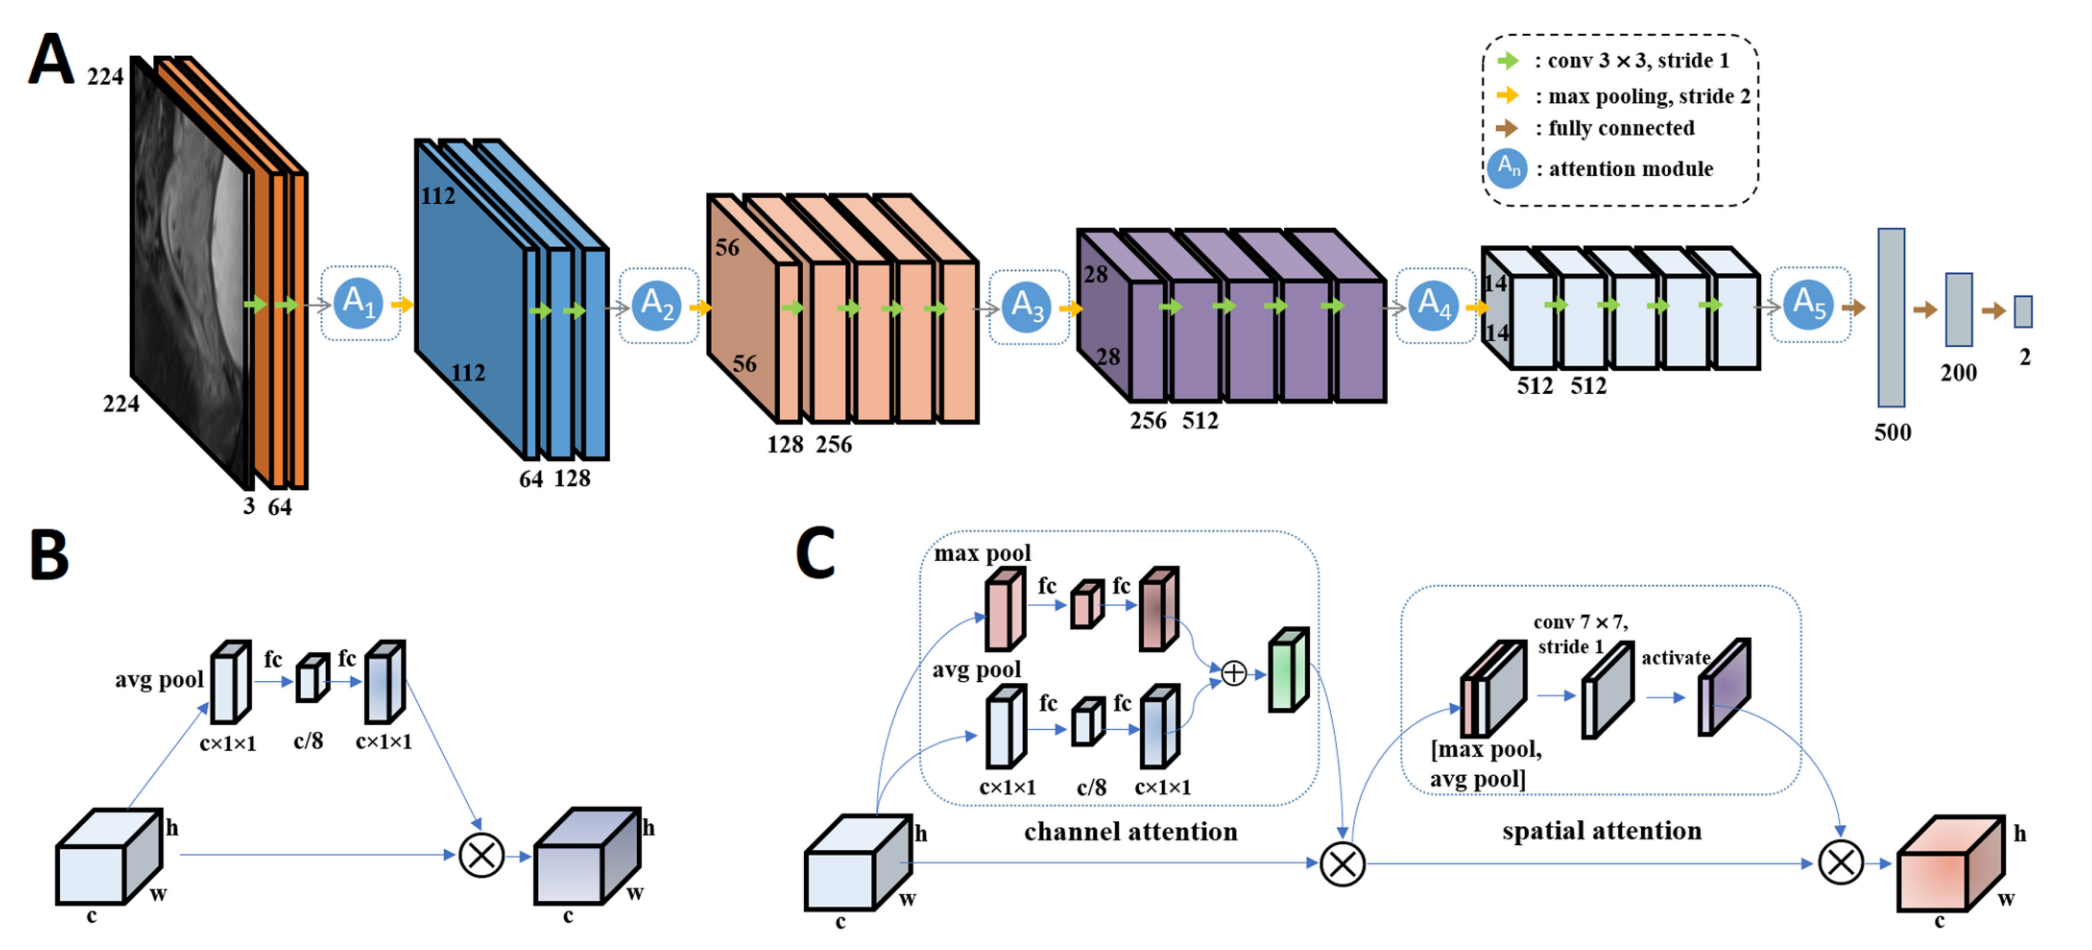
\includegraphics[width=0.8\textwidth]{figures/fig007.png}
    \caption*{Fonte: \cite{jiangMRIBasedRadiomics2021}}
    \label{fig:fig007}
\end{figure}

%---------------------------------------------------------
Em outro trabalho, \citeonline{renBiLSTMMultiheadAttentionbased2023}, desenvolveram um modelo avançado usando uma rede Bi-LSTM (memória de longo prazo bidirecional) combinada com um mecanismo de atenção de múltiplas cabeças, utilizando características radiômicas e imagens de \gls{tc} de lesões, para aprimorar a diferenciação dos principais subtipos de adenocarcinoma pulmonar, integrando assinaturas radiômicas com características radiológicas de tomografias computadorizadas. O estudo recrutou $421$ pacientes de três hospitais, confirmados com adenocarcinoma in situ, adenocarcinoma minimamente invasivo ou adenocarcinoma invasivo, com base na análise de $427$ lesões.

A metodologia empregada envolveu a extração de características radiômicas usando o software `\textit{PyRadiomics}' das regiões de lesões identificadas em cada imagem de \gls{tc}. As $100$ principais características foram então selecionadas por meio do método de classificação de características de máxima relevância e mínima redundância. Um modelo preditivo foi subsequentemente desenvolvido empregando essas características juntamente com as características radiológicas, usando a estrutura Bi-LSTM e atenção múltipla para classificar as lesões.

O desempenho diagnóstico do modelo foi quantitativamente impressionantes relativos aos modelos bases testados, alcançando valores da área sob a curva (AUC) de $0,985$, $0,94$ e $0,981$ nos grupos de treinamento, teste e validação, respectivamente, com precisão correspondentes a $0,92$, $0,976$ e $0,91$. Além disso, comparações foram feitas com dois outros modelos — \gls{cnn} em conjunto com atenção múltipla, e LSTM em conjunto com atenção múltipla — demonstrando que o modelo Bi-LSTM e atenção múltipla superou essas alternativas em precisão e acurácia no conjunto de testes.

Esta pesquisa destaca a potente combinação de técnicas avançadas de aprendizado de máquina com análises radiômicas e radiológicas detalhadas para refinar o processo diagnóstico para subtipos de adenocarcinoma pulmonar, potencialmente orientando abordagens de tratamento mais personalizadas baseadas na caracterização do subtipo.

%---------------------------------------------------------
 \citeonline{aiSelfAttentionBasedFusion2023} conduziram um estudo inovador intitulado ``Um Modelo de Fusão Baseado em Autoatenção de Características Radiômicas e Profundas para Previsão de Recorrência Precoce em Câncer de Pulmão de Células Não Pequenas'', que aborda o significativo desafio de prever a recorrência precoce deste câncer usando técnicas avançadas de aprendizado de máquina. Sua pesquisa aproveita o mecanismo de autoatenção para fundir características radiômicas manuais e características de aprendizado profundo extraídas de imagens de \gls{tc}, com o objetivo de aumentar a precisão preditiva e robustez para recorrência precoce em câncer de pulmão de células não pequenas.

O estudo começou empregando diversas técnicas de aprendizado de máquina para extrair uma variedade de características manuais de imagens de \gls{tc}, incluindo características de textura, forma e escala de cinza. Para capturar informações semânticas de alto nível e de representação, uma rede \textit{ResNet50} pré-treinada foi utilizada para a extração de características profundas. Essas características extraídas foram então fundidas com um vetor de características extraído de dados de texturas de imagens radiômicas e unificado usando um módulo de fusão de autoatenção inovador desenvolvido pelos pesquisadores. Este módulo otimiza e pondera o vetor de características fundidas, aproveitando plenamente o mecanismo de autoatenção para melhorar as capacidades de previsão do modelo e sua arquitetura pode ser conferida na Figura \ref{fig:fig008}.

Os resultados experimentais, avaliados no conjunto de dados público, \gls{tcia}, demonstraram que o modelo proposto superou significativamente os métodos existentes na previsão de recorrência precoce. O modelo exibiu melhorias substanciais em precisão de classificação, sensibilidade, especificidade e \gls{auc}, destacando seu potencial para guiar o tratamento em estágio inicial e melhorar as taxas de sobrevivência para pacientes com câncer de pulmão de células não pequenas.

Este estudo exemplifica a aplicação de técnicas avançadas de aprendizado de máquina em imagens médicas e oncologia, fornecendo um método robusto para a previsão de recorrência precoce que poderia impactar significativamente os resultados clínicos e as estratégias de tratamento em câncer de pulmão.

\begin{figure}[htbp]
    \centering
    \captionsetup{width=0.98\textwidth, justification=justified}
    \caption{Arquitetura Proposta por 
    \citeonline{aiSelfAttentionBasedFusion2023}, que emprega um Módulo de Fusão Baseado em Autoatenção (Self-attention based Fusion Module). O modelo integra características radiômicas, extraídas diretamente das imagens, com características de aprendizado profundo de uma rede ResNet50 pré-treinada. Ambas as vertentes de características passam por um processo de seleção (F-test) antes de serem concatenadas e processadas pelo módulo de autoatenção para a classificação final.}
    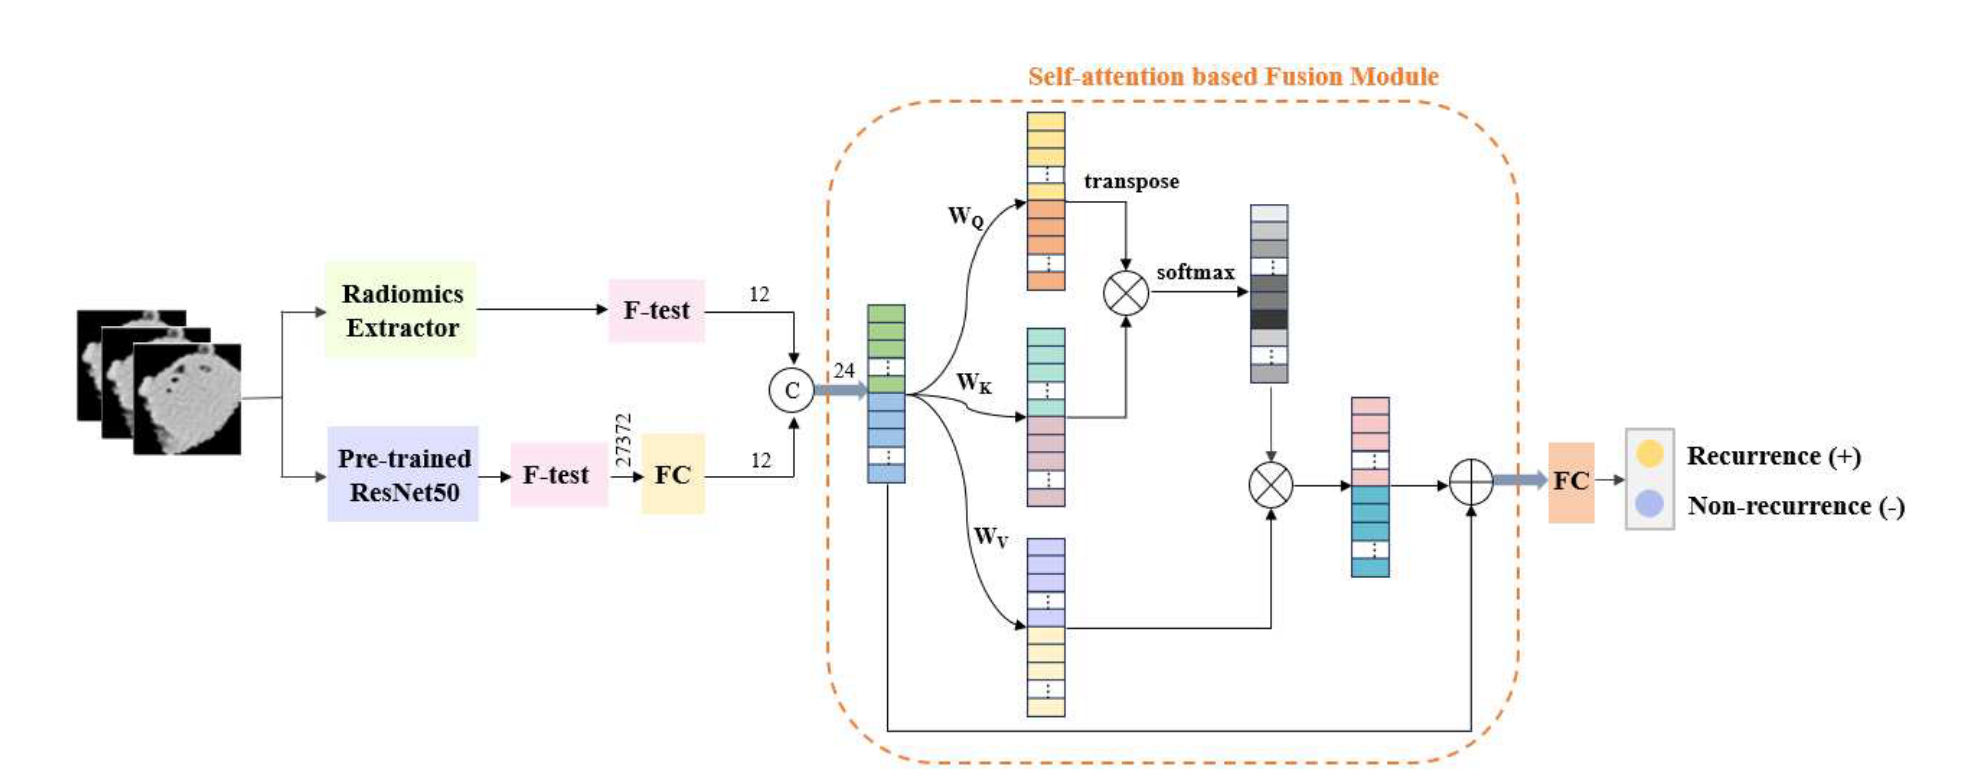
\includegraphics[scale=0.5]{figures/fig008.png}
    \caption*{Fonte: \cite{aiSelfAttentionBasedFusion2023}}
    \label{fig:fig008}
\end{figure}
%---------------------------------------------------------

\citeonline{iranmehrImprovedPredictionMGMT2022}
desenvolveram uma rede de aprendizado profundo inovadora que utiliza um mecanismo baseado em atenção para aprimorar a previsão do estado de metilação do gene MGMT em \gls{gbm}, o tipo mais agressivo de tumor cerebral. Pacientes com \gls{gbm} possuem uma expectativa muito baixa, entre 18 e 24 meses e requerem tratamentos agressivos, como por exemplo, quimioterapia. Sua pesquisa, apresentada em "\textit{Improved Prediction of MGMT Methylation Status in Glioblastoma using a Deep Attention Network}", destaca um avanço significativo nas capacidades diagnósticas não invasivas para \gls{gbm}, que tipicamente tem uma taxa de sobrevivência de apenas 18 meses.

O estudo foca no gene MGMT, cujo estado de metilação é crucial para determinar a eficácia da quimioterapia em pacientes com \gls{gbm}. As análises radiômicas tradicionais, embora úteis, muitas vezes não capturam os recursos intrincados necessários para uma previsão precisa da metilação. \citeonline{iranmehrImprovedPredictionMGMT2022} propõem um modelo que integra características radiômicas manuais com técnicas de \gls{ap}, melhorando a extração de características e a precisão da previsão de \gls{gbm}.

O modelo introduzido pela equipe utiliza uma combinação de mecanismos de atenção espremida e sequencial para priorizar fatias e regiões relevantes dentro das imagens de \gls{rmc}, respectivamente. Esse método não apenas melhora o foco em áreas significativas, mas também aprimora a interpretabilidade geral do modelo. O modelo proposto na Figura \ref{fig:fig009}, consiste de três etapas: 1) Um modelo base para extrair as características, 2) uma rede de atenção temporal e espacial e 3) uma rede de classificação para prever se o exame é metilado ou não metilado.
\newline

\begin{figure}[htbp]
    \centering
    \captionsetup{width=0.98\textwidth, justification=justified}
    \caption{Método proposto. \textit{DenseNet} é o modelo base, a saída da rede densa é alimentada pela rede de atenção que prioriza as fatias e regiões e gera a classificação binária do status de metilação do MGMT.
    }
    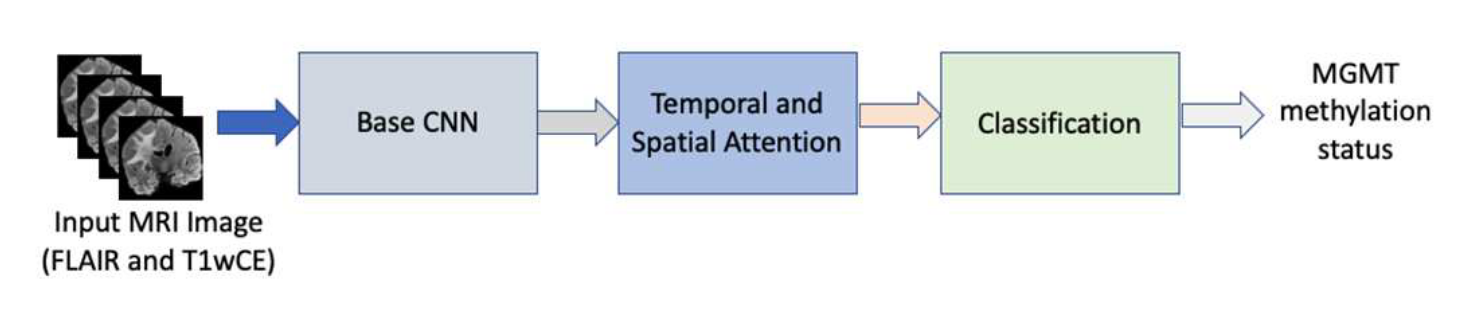
\includegraphics[width=1\textwidth]{figures/fig009.png}
    \caption*{Fonte: \cite{iranmehrImprovedPredictionMGMT2022}}
    \label{fig:fig009}
\end{figure}

O modelo base consiste em uma \textit{DenseNet} e segundo os autores, ela pode suportar milhares de camadas e ser resistente ao \textit{overfitting}. A saída da rede densa é fornecida para a rede espremida e autoatenção conforme mostrado na Figura \ref{fig:fig010}. Cada exame consiste em várias fatias e a atenção espremida priorizará fatias, usando o \textit{average pooling} global seguido por duas camadas densas separadas e depois o produto escalar com a entrada inicial. A saída da atenção espremida é fornecida à rede de autoatenção. Após a aplicação da autoatenção, o mapa de atenção contém \textit{pixels} com uma seção de maior importância em cada fatia. Com a rede de autoatenção, é possível enfatizar \textit{pixels} e regiões diferentes independente da distância em que estes \textit{pixels} se localizam na imagem. Múltiplas regiões com diferentes tamanhos, geradas a partir de regiões integrais, são então fornecidas à atenção sequencial. A rede de atenção sequencial adapta uma rede \gls{lstm}, que é capaz de aprender dependências de longo prazo. A saída passa por uma camada densa e uma função sigmoide para fins de classificação.

Avaliado em várias métricas de classificação binária, o modelo alcançou a melhor \gls{auc} de 70,59, demonstrando sua superioridade em relação aos métodos existentes. Este trabalho fornece uma abordagem robusta e automática para capturar características críticas de imagens de ressonância magnética, avançando significativamente na previsão do estado de metilação em \gls{gbm} em comparação com métodos anteriores. As implicações de tais avanços são profundas, potencialmente melhorando o planejamento de tratamentos personalizados e, em última análise, os resultados para os pacientes com glioblastoma.

\begin{figure}[htbp]
    \centering
    \captionsetup{width=0.98\textwidth, justification=justified}
    \caption{Arquitetura Proposta por \citeonline{iranmehrImprovedPredictionMGMT2022} para análise de mapas de características convolucionais, que inclui bloco \gls{se} e autoatenção, segmentação de regiões integrais (representadas pelas áreas em verde e vermelho), além de uma camada \gls{lstm}. O modelo também utiliza diferentes tipos de atenção para focar em regiões específicas dos dados.
    }
    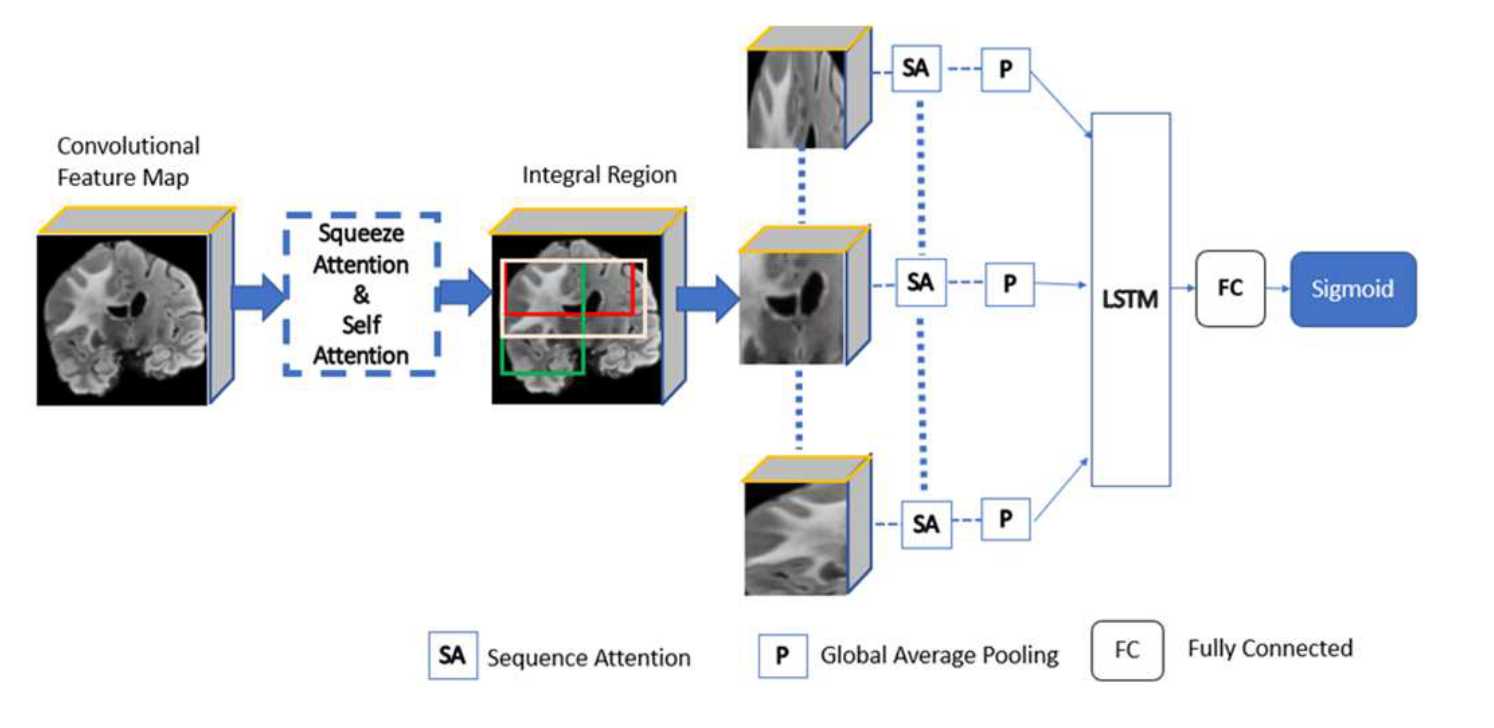
\includegraphics[width=1\textwidth]{figures/fig010.png}
    \caption*{Fonte: Adaptado de \cite{iranmehrImprovedPredictionMGMT2022}}
    \label{fig:fig010}
\end{figure}


Por fim, \citeonline{yangNeuralNetworkDesign2024a} demonstram como o mecanismo de atenção auxilia as redes neurais a se concentrar em informações pertinentes nos dados, e sua integração com redes neurais convolucionais aprimora as capacidades de extração de características do modelo como um todo. O trabalho destaca que o mecanismo de atenção pode ser ser categorizado em: mecanismo de atenção seletiva e mecanismo de autoatenção.

O mecanismo de atenção seletiva gera um conjunto de pesos de atenção ao prever diretamente a importância de cada parte dos dados em relação ao objetivo da tarefa, adicionando os pesos ponderadamente aos dados de entrada para realçar as informações importantes e suprimir as informações irrelevantes nos dados. A \gls{se}Net é um trabalho representativo nos mecanismos de atenção seletiva. A \gls{se}Net propõe um mecanismo de atenção no domínio dos canais que aprende o valor dos pesos para cada canal no mapa de características, a fim de realçar ou suprimir cada característica do canal. O mecanismo de atenção seletiva é orientado para os objetivos da tarefa e otimiza diretamente as características, mas carece da capacidade de extrair informações globais. O mecanismo de autoatenção consegue capturar informações globais, mas sofre com alta complexidade e dificuldades de otimização. 

\citeonline{yangNeuralNetworkDesign2024a} propuseram um algoritmo com módulo de busca de atenção diferenciável, assim a rede pode extrair as informações cognitivas e semântica das características da imagem. Em seguida, um espaço de busca multi-atenção é estabelecido englobando seis operações de atenção consolidadas em um único módulo de busca. Por fim, para aprimorar a eficiência, o espaço de busca, antes discreto, é convertido para contínuo, empregando um algoritmo de busca diferencial para identificar a rede de atenção ótima. Para validar os resultados, foi aplicada a classificação em imagens  muito detalhadas. 

Como resultado o método alcançou acurácia de 87,4\% no conjunto de dados CUB-200-2011 que consiste em mais de 11 mil imagens de pássaros distribuídas em 200 classes, apresentando um ganho de desempenho de 1,1\%, 0,9\% e 2,1\% em relação ao módulo de atenção seletiva por canal, ao módulo de atenção seletiva espacial e ao módulo de autoatenção espacial, respectivamente. Por fim, os autores concluem que o módulo de atenção encontrado incorpora as vantagens de diferentes mecanismos de atenção e pode ajudar o modelo a melhor extrair e utilizar características discriminativas \cite{yangNeuralNetworkDesign2024a}.

%--------------------------------------------------------
\section{CONSIDERAÇÕES FINAIS DO CAPÍTULO}
\label{sec:consideracoes_finais}

Os métodos de avaliação de imagens médicas, tanto via análise radiômica por extração de textura quanto por aprendizado profundo obtiveram êxito em análise de imagens médicas. Vale pontuar que estas técnicas de Aprendizado de Máquina, utilizando dados de textura podem ser insuficientes em capturar a complexidade e diversidade de informações a cerca do ventrículo como também pode ser afetada pela qualidade da imagem. Métodos de aprendizado profundo podem aprender automaticamente semânticas de alto nível e informações representativas de imagens de \gls{rmc} sem necessidade de características extraídas manualmente.
Métodos de aprendizado profundo tem obtido ótimos resultados em diagnósticos, segmentação, estadiamento e prognósticos, todavia o mesmo tem suas limitações como a baixa quantidade no conjunto de dados, um desafio geral na área médica, \textit{overfitting} e pouca interpretabilidade do modelo em si \cite{pontoneClinicalApplicationsCardiac2022}.

Dadas as vantagens e limitações discutidas, este trabalho tem como proposta a fusão de uma arquitetura de aprendizado profundo baseada no mecanismo de atenção que integra características radiômicas e profundas para a identificação de cardiomiopatias. 

\chapter{Trabalhos Relacionados}
\label{chap:metodologia}
\vspace{-\baselineskip} %Manter para garantir o espaçamento da biblioteca.


A metodologia deste trabalho visa propor e investigar arquiteturas de \gls{ap} que unificam características radiômicas e características profundas. O modelo base selecionado é uma versão adaptada do trabalho de \cite{aiSelfAttentionBasedFusion2023}, mencionado nos trabalhos relacionados e o esquemático de sua arquitetura pode ser visto na Figura \ref{fig:fig008}. Importante ressaltar que o trabalho em questão é aplicado no cenário de câncer de pulmão de células não pequenas em imagens de \gls{tc} e este trabalho pretende aplicar o mesmo estudo no cenário de cardiomiopatia sendo este o modelo linha de base. Também serão aplicado adaptações a esta arquitetura original como: quantidade de execuções nos transformers, aumento dos vetores profundos e radiômicos, mudança na forma de concatená-los, entre outros.

 Os experimentos foram divididos em duas fases manuais. Na primeira fase, foi aplicado o modelo base, ao conjunto de dados público selecionado. Na etapa de pré-processamento desta fase, foram aplicadas diversas técnicas de aprendizado de máquina para extrair características manuais de imagens de \gls{rmc} e sua respectiva máscara, abrangendo textura, forma, escala de cinza, etc. Estas características serão chamadas, deste ponto em diante, de características radiômicas. Seguindo com o pré-processamento, as imagens de \gls{rmc} foram processadas por uma rede \textit{ResNet50} pré-treinada, extraindo características que serão intituladas de características profundas. As características profundas encapsulam informações semânticas de alto nível e de representação das imagens de \gls{rmc}. Estas características, radiômicas e profundas, são então fundidas em um vetor de características unificado e aplicado a um único bloco de autoatenção, e obtendo ao fim da arquitetura do modelo base, as classificação indicando se há ou não cardiomiopatia, ou seja, uma classificação binária.

Na segunda fase, diversas adaptações foram aplicadas ao modelo base com o intuito de aprimorar a robustez e a acurácia. Algumas das adaptações feitas consistem no aumento do tamanho dos vetores semânticos, também conhecidos na literatura como \textit{embeddings}, seu tamanho foi variado também entre $12$, $24$, $48$ e $64$, valores testados de forma análoga a um hiperparâmetro, com a premissa de preservar mais das informações originais ao custo do aumento quase irrelevante de custo computacional.

A concatenação dos \textit{embeddings} também foi adaptada se comparada ao modelo original. Na versão original a concatenação se dá na última dimensão enquanto que nas versões adaptadas se dá na primeira dimensão. Em termos práticos, na versão original dois vetores $1\text{x}12$ concatenados resultam em $1\text{x}24$, na abordagem adaptada resultam em $2\text{x}12$. 

A mudança na forma de concatenar é feita de forma proposital pois a versão adaptada conta com uma camada convolucional inédita se comparada com a versão original, visando extrair informação relevante da junção dos \textit{embeddings}. A versão adaptada adiciona também uma camada de atenção seletiva no formato de um bloco \gls{se} que precede o bloco de autoatenção. Outra mudança na versão adaptada é o bloco de autoatenção ser aplicado $N$ vezes ao invés de uma única vez como acontece no modelo base trazendo uma perceptível melhora nos resultados. Como o número de vezes que um bloco é executado aumenta respectivamente o tamanho da rede, será testado com alguns valores numéricos de forma incremental para dosar os resultados e evitar sobreajuste. Lembrando que ambos mecanismos de atenção tem propostas diferentes, enquanto o bloco de atenção seletiva atua na relação entre os canais dos \textit{embeddings}, o bloco de autoatenção otimiza e pondera o vetor de características fundidas de forma eficaz. A intuição de aplicar mecanismos de atenção com propósitos diferentes vem do trabalho de \cite{yangNeuralNetworkDesign2024a}. 

A Figuras \ref{fig:fig015-01} e \ref{fig:fig015-02} demonstram o fluxograma do projeto na fase de pré-processamento e o fluxograma da execução da arquitetura proposta respectivamente.

\begin{figure}[H]
    \centering
    \captionsetup{width=0.98\textwidth, justification=justified}
    \caption{Fluxograma - Pré-Processamento e Arquitetura}
    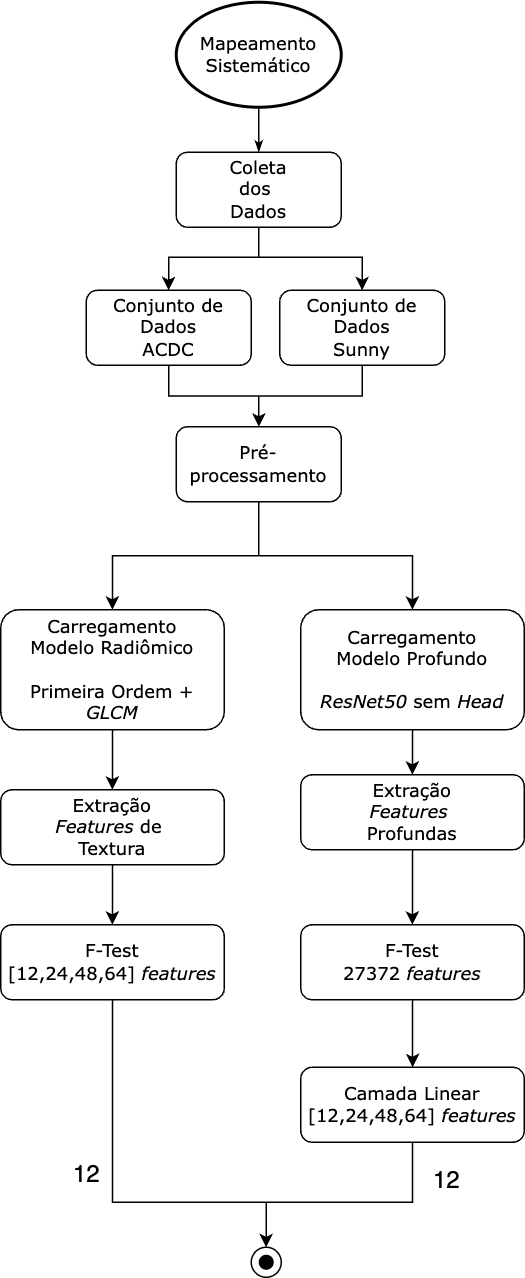
\includegraphics[scale=0.38]{figures/fig015-01.png}
    \caption*{Fonte: Autor}
    \label{fig:fig015-01}
\end{figure}

\begin{figure}[H]
    \centering
    \captionsetup{width=0.98\textwidth, justification=justified}
    \caption{Fluxograma - Continuação}
    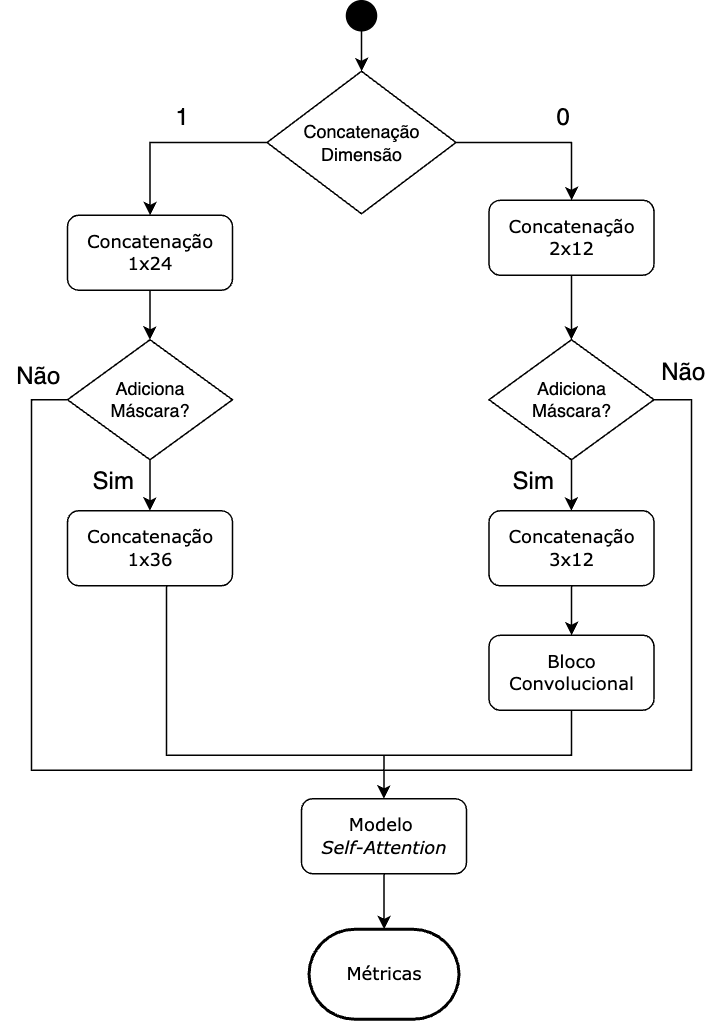
\includegraphics[scale=0.36]{figures/fig015-02.png}
    \caption*{Fonte: Autor}
    \label{fig:fig015-02}
\end{figure}

%--------------------------------------------------------
\section{BASES DE DADOS} 
\label{subsec:cap4_dataset}

Duas bases de dados foram utilizadas no experimento: o primeiro conjunto de dados é o \gls{acdc}\footnote{https://www.creatis.insa-lyon.fr/Challenge/acdc/databases.html}. O segundo conjunto de dados é o SunnyBrook Cardiac Data (SCD) \footnote{https://www.cardiacatlas.org/sunnybrook-cardiac-data} \cite{radauEvaluationFrameworkAlgorithms2009}. Ambos conjuntos de dados são públicos e destinados a pesquisa.

O conjunto de dados ACDC é composto por $150$ imagens sendo $100$ para treino e $50$ para testes distribuídas em 5 classes igualmente distribuídas: \gls{dcm}, \gls{hcm}, \gls{nor}, \gls{minf} e \gls{rv}. O conjunto de dados SunnyBrook é composto por $45$ imagens sendo e, respeitando as proporções determinadas no ACDC, foram escolhidas $30$ imagens para treino e $15$ para testes. As classes são NOR, IC, IC-I e HIP. Detalhes das classes são descritas nas seções que seguem destinadas a cada conjunto de dados.

%--------------------------------------------------------
\subsection{Conjunto de Dados ACDC} 
\label{subsec:cap4_acdc}

O conjunto de dados \gls{acdc} foi criado a partir de exames clínicos reais adquiridos no hospital universitário de Dijon (França). Os dados adquiridos foram totalmente anonimizados e tratados de acordo com as regulamentações estabelecidas pelo comitê ético local do hospital de Dijon. O conjunto de dados cobre várias patologias bem definidas com casos suficientes para (1) treinar adequadamente métodos de aprendizado de máquina e (2) avaliar claramente as variações dos principais parâmetros fisiológicos obtidos a partir de cine-RM (em particular volume diastólico e fração de ejeção). O conjunto de dados é composto por $150$ exames (todos de pacientes diferentes) divididos em cinco subgrupos distribuídos de forma igualitária, sendo quatro patológicos e um grupo de sujeitos saudáveis. Cada exame é composto por um número variável de imagens que compõem o volume do coração. Dentre as cinco classes distintas, tem-se: \gls{dcm}, \gls{hcm}, \gls{nor}, \gls{minf} e \gls{rv}. As classes \gls{dcm} e \gls{hcm} são interpretadas como passíveis de \gls{car} e as demais; \gls{nor}, \gls{minf} e \gls{rv}; são interpretadas como o coração em condições sem cardiomiopatia, os detalhes das classes podem ser verificados na Tabela \ref{tab:conditions}. 

As máscara de segmentação também acompanham o conjunto de dados, para possíveis aplicações de segmentação. Os valores dos rótulos variam de $0$ a $3$ e representam voxels pertencentes ao fundo (0), à cavidade do ventrículo direito (1), ao miocárdio (2) e à cavidade do ventrículo esquerdo (3). As Figuras \ref{fig:fig033-01}, \ref{fig:fig033-02} e \ref{fig:fig033-03} representam as imagens e suas máscaras das classes \gls{dcm}, \gls{hcm} e \gls{nor}. Nas máscaras é possível ver três níveis de tons de cinza respectivos a segmentação citada.

\begin{table}[H]
    \centering
    \caption{Classes ACDC -Descrição}
    \renewcommand{\arraystretch}{1} % default é 1 
    \begin{tabular}{|>{\centering\arraybackslash}p{2cm}|p{12cm}|}
    \hline 
          % \textbf{Condição} & \textbf{Descrição} & Característica \\ 
          % \textbf{Condição} & \textbf{Descrição} \\ 
          \multicolumn{1}{|c|}{\textbf{Condição}} & \multicolumn{1}{c|}{\textbf{Descrição}} \\
          & \\
    \hline 
        \textbf{DCM} &
        A cardiomiopatia dilatada é uma condição em que o coração se 
        torna dilatado e não consegue bombear o sangue de forma
        eficiente. 
        \newline \newline
        \textbf{Característica}: O ventrículo esquerdo está dilatado e com função sistólica reduzida de acordo com seu tamanho original. \\ 
    \hline
        \textbf{HCM} & 
        A cardiomiopatia hipertrófica é uma condição onde há um espessamento anormal do músculo cardíaco, especialmente do ventrículo esquerdo. 
        \newline \newline
        \textbf{Característica}: A parede do ventrículo esquerdo está significativamente espessada, o que pode restringir o volume sanguíneo e o fluxo de saída. \\ 
    \hline
        \textbf{NOR} & 
        Esta classe representa corações normais (sem cardiomiopatia) sem qualquer condição patológica. 
        \newline \newline
        \textbf{Característica}: Estruturas e funções cardíacas normais, sem dilatações ou hipertrofias significativas. \\ 
    \hline
        \textbf{MINF} & 
        O infarto do miocárdio, ou ataque cardíaco, ocorre quando o fluxo sanguíneo para uma parte do coração é bloqueado por um período suficiente para causar danos ao músculo cardíaco. 
        \newline \newline
        \textbf{Característica}: Áreas do coração mostram cicatrizes ou fibrose devido ao infarto anterior, frequentemente visível nas imagens de ressonância magnética. \\ 
    \hline
        \textbf{RV} & 
        A hipertrofia do ventrículo direito é uma condição em que o ventrículo direito do coração está aumentado. 
        \newline \newline
        \textbf{Característica}: Espessamento da parede do ventrículo direito, que pode ser devido a diversas condições, como hipertensão pulmonar ou doenças congênitas do coração. \\
    \hline
    \end{tabular} 
    \caption*{Fonte: Adaptado de \cite{bernardDeepLearningTechniques2018a}}
    \label{tab:conditions}
\end{table}


Os dados tem composição balanceada e sua distribuição pode ser conferida na Tabela \ref{tab:count_dataset}. É possível notar, que após o agrupamento das classes como especificado, estas tornam-se minimamente desbalanceadas, em uma proporção de $40/60$. As informações de cada paciente também é composta pelas seguintes informações: peso, altura, bem como o instante da fase diastólica e sistólica \cite{bernardDeepLearningTechniques2018a} que neste trabalho não são utilizadas dado o fato de ser tratado apenas as imagens médicas.

\begin{table}[H]
    \centering
    \caption{Classes do ACDC}
    \renewcommand{\arraystretch}{1} % default é 1 
    \begin{tabular}{|c|c|c|c|}
    \hline 
          \textbf{Grupo} & \textbf{Quantidade} & \textbf{C/ CM} & \textbf{S/ CM}  \\ 
    \hline 
        NOR & 30 & 0 & 30 \\ 
        DCM & 30 & 30 & 0\\ 
        HCM & 30 & 30 & 0\\ 
        MINF & 30 & 0 & 30 \\ 
        RV & 30 & 0 & 30 \\
    \hline 
        \textbf{Total}: & 150  & 60 & 90\\ 
    \hline 
    \end{tabular} 
    \caption*{Fonte: Autor}
    \label{tab:count_dataset}
\end{table}


\begin{figure}[H]
    \centering
    \captionsetup{width=0.98\textwidth, justification=justified}
    \caption{Imagem médica da classe DCM e sua respectiva máscara}
    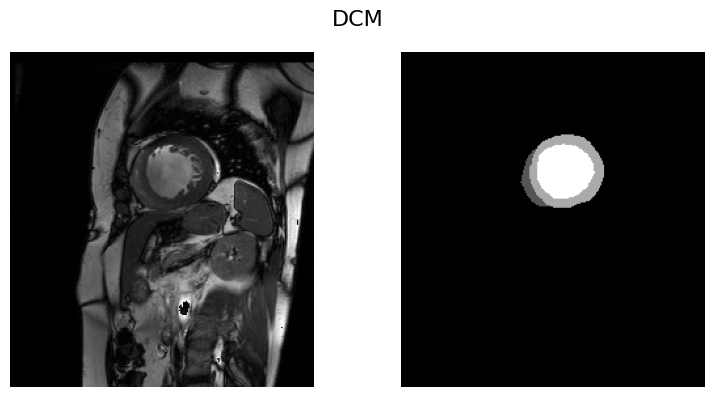
\includegraphics[width=0.8\textwidth]{figures/fig033-01.png}
    \caption*{Fonte: Autor}
    \label{fig:fig033-01}
\end{figure}

\begin{figure}[H]
    \centering
    \captionsetup{width=0.98\textwidth, justification=justified}
    \caption{Imagem médica da classe HCM e sua respectiva máscara}
    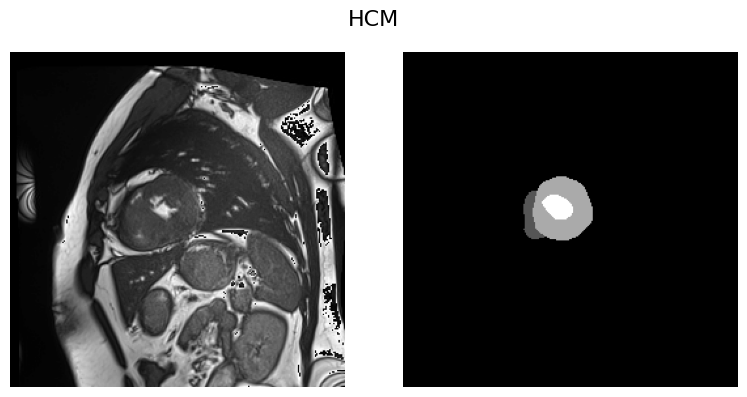
\includegraphics[width=0.8\textwidth]{figures/fig033-02.png}
    \caption*{Fonte: Autor}
    \label{fig:fig033-02}
\end{figure}

\begin{figure}[H]
    \centering
    \captionsetup{width=0.98\textwidth, justification=justified}
    \caption{Imagem médica da classe NOR e sua respecitva máscara}
    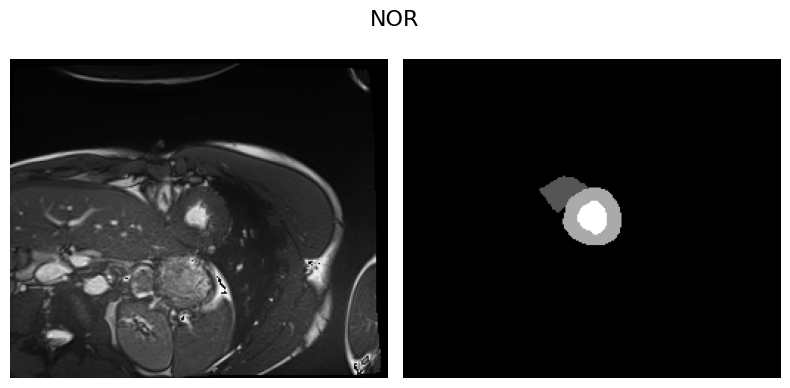
\includegraphics[width=0.8\textwidth]{figures/fig033-03.png}
    \caption*{Fonte: Autor}
    \label{fig:fig033-03}
\end{figure}

% --------------------------------------------------------
\subsection{Conjunto de Dados Sunny} 
\label{subsec:cap4_sunny}

O conjunto de dados Sunny, também conhecidos como \textit{2009 Cardiac MR Left Ventricle Segmentation Challenge data}, consiste em 45 imagens de RM de um grupo misto de pacientes e patologias: saudáveis, hipertrofia, insuficiência cardíaca com infarto e insuficiência cardíaca sem infarto. Um subconjunto desses dados foi utilizado pela primeira vez no desafio de segmentação automatizada do miocárdio a partir de imagens de RM em eixo curto, realizado em um workshop do MICCAI em 2009 \cite{radauEvaluationFrameworkAlgorithms2009}. 

Há quatro grupos patológicos neste conjunto de dados, que foram classificados no seguinte formato:

\begin{enumerate}
    \item Insuficiência cardíaca com infarto (\textbf{IC-I}): grupo com \gls{fe} < $40$\% e evidência de realce tardio com gadolínio (Gd);
    \item Insuficiência cardíaca sem infarto (\textbf{IC}): grupo com \gls{fe} < $40$\% e sem realce tardio com gadolínio;
    \item Hipertrofia do ventrículo esquerdo (\textbf{HIP}): grupo com \gls{fe} normal (> $55$\%) e uma razão de massa do ventrículo esquerdo sobre a área da superfície corporal > $83$ g/m²;
    \item Sem cardiomiopatia (\textbf{NOR}): grupo com \gls{fe} > $55$\% e sem hipertrofia.
\end{enumerate}

\noindent Para o presente trabalho foram utilizadas as classes \textbf{HIP} e \textbf{NOR} para classificação de cenário com e sem cardiomiopatia respectivamente. A Tabela \ref{tab:sunny_stats} demonstra como se encontram distribuídos os $45$ pacientes e os valores relacionados as atividades cardiovasculares utilizados para fins de classificação dos pacientes:
\newline

\begin{table}[h!]
\centering
\caption{Estatísticas dos volumes e função do ventrículo esquerdo (média).}
\begin{tabular}{@{}lcccc@{}}
\toprule
\textbf{}  & \textbf{NOR (n=9)} & \textbf{HIP (n=12)} & \textbf{IC (n=12)} & \textbf{IC-I (n=12)} \\ \midrule
\textbf{Vol. Diastólico Final (ml)} & 115.69 (36.89)   & 114.39 (50.46)      & 233.67 (63.21)     & 244.92 (86.02)       \\
\textbf{Vol. Sistólico Final (ml)}  & 43.10 (14.74)    & 43.11 (24.50)       & 158.28 (56.34)     & 174.34 (90.64)       \\
\textbf{Fração de Ejeção (\%)}        & 62.93 (3.65)     & 62.72 (9.22)        & 33.09 (13.07)      & 32.01 (12.27)        \\
\textbf{Massa Ventrículo Esq. (g)} & 130.27 (32.69)   & 175.87 (85.70)      & 193.69 (39.01)     & 201.32 (45.24)       \\ \bottomrule
\end{tabular}
\caption*{Fonte: Adaptado de \cite{radauEvaluationFrameworkAlgorithms2009}.}
\label{tab:sunny_stats}
\end{table}

%---------------------------------------------------------
\section{PRÉ-PROCESSAMENTO}
\label{subsec:cap4_preprocess}

Na fase de pré-processamento, foi utilizado o conjunto de dados \gls{acdc}. O \gls{acdc} originalmente tem cinco classes distintas e foi agrupado de forma que DCM e HCM indicam a classe CAR e os demais rótulos NOR, MINF e RV, são classificados como sem cardiomiopatia. O conjunto de \textit{frames} utilizados são definidos na fase diastólica e a quantidade de \textit{frames} é variada para cada paciente de acordo como consta no conjunto de dados. As características radiômicas são extraídas utilizando a biblioteca \textit{PyRadiomics}\footnote{https://pyradiomics.readthedocs.io}. Utilizando esta ferramenta, pode-se enviar como entrada o volume 3D das imagens cardíacas e suas respectivas máscaras e obter as características manuais extraídas abrangendo textura, forma, escala de cinza, etc. O resultado é um vetor com $\RadiomicFeatures$ características radiômicas. As características profundas são extraídas através de uma rede ResNet50 sem a última camada responsável pela classificação. Este processo é aplicado para cada fatia do volume 3D tanto para imagem cardíaca quanto para sua respectiva máscara tendo como resultado final vetores de tamanho $\DeepFeatures$. 

Seguindo a receita do modelo base, é aplicado o \textit{F-Test} para redução de dimensionalidade das características profundas de $\DeepFeatures$ para $\DeepFeaturesPostLinear$ e das características radiômicas de $\RadiomicFeatures$ para $\text{EMBED}_{size} \in \{24, 48, 64\}$. O valor de $\text{EMBED}_{size}$ varia nas versões adaptadas, sendo considerado um hiperparâmetro, e garante que todos os \textit{embeddings} possuam o mesmo valor. A concatenação é feita na última dimensão para o teste com modelo original e suas variações, e na primeira dimensão para as versões adaptadas. Vale ressaltar que diferente da versão do modelo base que só possui um vetor de características profundas, nas versões adaptadas pode-se ter um vetor adicional referente a máscara com a região de interesse. 

%---------------------------------------------------------
\section{EXTRAÇÃO DE CARACTERÍSTICAS RADIÔMICAS}
\label{subsec:cap4_caracteristicas_radiomicas}

Foram extraídas características radiômicas da fase da diástole\footnote{A diástole corresponde à parte do ciclo cardíaco caracterizada pelo relaxamento muscular e enchimento dos ventrículos \cite{brielerCardiomyopathyOverview2017}}, representada por um conjunto de fatias variando entre $6$ e $18$ \textit{frames}, de cada paciente usando \gls{glcm} e estatísticas baseadas em histograma. Será aplicado o filtro \gls{log} com cinco valores diferentes em cada parte para suavizar as imagens e realçar as bordas. Foram calculadas características \gls{glcm} como contraste, entropia, correlação, homogeneidade e energia para cada filtro \gls{log}. Também são calculadas características de intensidade como média, variância, média dos percentis (10 e 90), desvio robusto da média absoluta, curtose e assimetria usando estatísticas de primeira ordem. Foram obtidos $\RadiomicFeatures$ características radiômicas para cada paciente dentro da quantidade de fatias extraídas na fase diastólica.

%---------------------------------------------------------
\section{EXTRAÇÃO DE CARACTERÍSTICAS PROFUNDAS}
\label{subsec:cap4_caracteristicas_profundas}
 
Para extrair características profundas das imagens de \gls{rmc}, foi utilizada a arquitetura pré-treinada de um \textit{ResNet50} sem sua última camada totalmente conectada e com os pesos congelados. A \textit{ResNet50} é um modelo de rede neural convolucional profunda com 50 camadas que compreende muitos blocos residuais. Cada bloco contém módulos de convolução e uma conexão de salto que transfere a informação do bloco anterior para o próximo bloco. A conexão de salto ajuda a reter a informação semântica mais básica aprendida nas camadas anteriores, que de outra forma se tornaria abstrata devido à conexão de longa cadeia. A conexão de salto também evita o desaparecimento do gradiente nas camadas mais profundas ao fornecer um caminho alternativo para a retropropagação. A informação da conexão de salto é adicionada à informação calculada em cada bloco \cite{aiSelfAttentionBasedFusion2023}. Ao todo são $\DeepFeatures$ características coletadas da saída deste modelo.

%---------------------------------------------------------
\section{CONCATENAÇÃO}
\label{subsec:cap4_concatenacao}

Em posse das características radiômicas, é aplicado um \textit{F-Test} tanto às $\RadiomicFeatures$ características radiômicas quanto às $\DeepFeatures$ características profundas, reduzindo cada um dos vetores ao espaço dimensional especificado. No método de fusão convencional, simplesmente é concatenado os dois vetores de características como na Equação \ref{eq:concat}, onde \textit{Concat} simplesmente concatena os dois vetores. Unificando os vetores, o resultado é baseado na dimensão escolhida de concatenação escolhida. O resultado é enviado aos mecanismos de atenção, sendo este o bloco de autoatenção no modelo original e o bloco convolucional seguido do bloco de autoatenção no modelo adaptado.

\begin{equation}
F_{hd} = \textit{Concat}(F_h, F_d, dim) \quad dim \in \{0,1\}
\label{eq:concat}
\end{equation}

%---------------------------------------------------------
\section{MÓDULO DE ATENÇÃO SELETIVA}
\label{subsec:cap4_mod_selective_attn}

A atenção seletiva desempenha um papel crucial na melhoria do desempenho de modelos de aprendizado profundo ao permitir que eles foquem em características mais relevantes nas representações internas. Especificamente, o bloco \gls{se} é projetado para recalibrar adaptativamente os canais das representações, atribuindo pesos maiores às características mais informativas. Esse mecanismo opera em duas etapas principais: primeiro, reduz a dimensionalidade das características globais (\textit{squeeze}) para capturar o contexto geral, e, em seguida, aplica um mecanismo de excitação (\textit{excitation}) para ajustar os pesos de cada canal com base na importância relativa. Ao integrar blocos SE em uma arquitetura, o modelo pode aprimorar sua capacidade de discriminar padrões relevantes e suprimir ruídos ou informações irrelevantes, resultando em maior precisão e eficiência no processamento dos dados \cite{huSqueezeandExcitationNetworks2018}.

Sendo o bloco \gls{se} adicionado apenas na versão adaptada, visando aprimorar os resultados, o vetor resultante da concatenação é $3\times64$ se assumirmos $\text{EMBED}_{size}$ igual a $64$ e a adição da máscara. Uma camada convolucional 1D é aplicada, com número de canais igual a $16$, \textit{kernel} igual a 3, \textit{stride} igual a $1$ e \textit{padding} igual a $1$ para não diminuir as dimensões após o processamento. Tendo como resultado da primeira convolução $16$ canais, é aplicado o bloco \gls{se} para identificar os canais mais relevantes e escalar a entrada original. O bloco \gls{se} possui o parâmetro $r$ de redução de dimensionalidade a ser configurado e foi utilizado o valor $16$ conforme os autores do artigo original sugerem. Outra convolução 1D é aplicada com um único canal, assim tem-se vetor resultante de uma única dimensão que pode servir como entrada para o próximo bloco, o de autoatenção.

%---------------------------------------------------------
\section{MÓDULO DE AUTOATENÇÃO}
\label{subsec:cap4_mod_self_attnn}

O mecanismo de autoatenção foi empregado com a responsabilidade de aprender a importância de cada característica e capturar suas dependências de longo alcance. Como ilustrado na Figura \ref{fig:fig011}, o módulo de autoatenção é utilizado para mapear uma consulta ($Q$), chave ($K$) e valor ($V$) para um valor de atenção. São utilizadas $24$ características concatenadas $F_{hd}$ no modelo original e $\text{EMBED}_{size}$ características nas versões adaptadas. Do vetor resultante, é projetada cada característica em três matrizes aprendíveis: matriz chave $K$, matriz consulta $Q$ e matriz de valor $V$ pelo produto escalar com suas respectivas matrizes de peso $W_{Q}$, $W_{K}$ e $W_{V}$. Logo os valores $Q$, $K$, $V$ são denotados como $W_{Q}F_{gd}$, $W_{K}F_{gd}$, $W_{V}F_{gd}$ respectivamente, onde $W_{Q}$, $W_{K}$ e $W_{V}$ representam a transformação linear para as matrizes $Q$, $K$ e $V$. 

O módulo de autoatenção é definido na Equação \ref{eq:attention}, em que $d_{k}$ é a dimensão do valor de $K$. Sem utilizar operações recorrentes ou convolucionais em específico, o módulo de autoatenção pode modelar as dependências de longo prazo entre as características de entrada.
Este módulo calcula de forma adaptativa os pesos entre as características com base em sua importância e relevância, capturando de forma mais abrangente as associações entre características radiômicas e profundas. Tal processo realça a capacidade expressiva das características fundidas e permite que o modelo foque mais precisamente nas características mais informativas que auxiliam a diagnosticar imagens médicas e reduzir a influência de características irrelevantes nesta previsão. Além disso, o modelo pode alocar dinamicamente atenção a diferentes amostras de imagens de \gls{rmc}. Essa flexibilidade permite com que o modelo se adapte melhor à representação de características de diferentes amostras, melhorando a precisão e a generalização.

A função de perda utilizada utilizada no modelo é a função de entropia cruzada binária, do termo  \gls{bce}, que é calculada pela Equação. \ref{eq:bce} onde $\mathcal{L}_{bce}$ denota o \gls{bce}, $N$ denota o número de imagens de \gls{rmc} vistas em tempo de treinamento, $r$ denota a classe alvo de \gls{car} e $\hat{r}$ o valor previsto pelo modelo de \gls{car}, 1 indica indícios de \gls{car} e 0 sua ausência.

\begin{equation}
\mathcal{L}_{bce} = -\frac{1}{N} \sum_{i=1}^N
(r_i \ln \hat{r}_i + (1 - r_i) \ln (1 - \hat{r}_i))
\label{eq:bce}
\end{equation}

%---------------------------------------------------------
\section{MÉTRICAS}
\label{subsec:cap4_metrics}
Para medir o desempenho da solução serão aplicadas as seguintes métricas: acurácia, precisão, revocação expressas pelas Equações \ref{eq:acc}, \ref{eq:precision} e \ref{eq:recall} respectivamente.

Também foi calculada a \gls{auc}, que consistem em um gráfico com a habilidade de validar um classificador binário. Esta curva é criada plotando, em gráfico, a taxa de verdadeiros positivos (TPR) contra a taxa de falsos positivos (FPR) em diversos limites contínuos de decisão. A equação da \gls{auc} é apresentada na Equação \ref{eq:auc} em formato contínuo embora seja prática comum discretizá-lo.


\begin{equation}
  \textit{Acurácia} = \frac{\textit{TP} + \textit{TN}}{\textit{TP} + \textit{TN} + \textit{FP} + \textit{FN}}
  \label{eq:acc}
\end{equation}

\begin{equation}
  \textit{Precisão} = \frac{\textit{TP}}{\textit{TP} + \textit{FP}}
  \label{eq:precision}
\end{equation}

\begin{equation}
  \textit{Revocação} = \frac{\textit{TP}}{\textit{TP} + \textit{FN}}
  \label{eq:recall}
\end{equation}

\begin{equation}
  \text{AUC} = \int_{x=0}^{1} \text{TPR}(\text{FPR}^{-1}(x)) \ \, d(x)
  \label{eq:auc}
\end{equation}

%---------------------------------------------------------
\section{ARQUITETURA PROPOSTA}
\label{subsec:cap4_architecture}

% A arquitetura proposta é composta por: extração de características radiômicas e profundas; redução de dimensionalidade para que ambas possuam tamanhos similares, aplicação dos mecanismos de atenção seletivo e autoatenção e classificação binária do resultado.

O esquemático da arquitetura proposta é observado na Figura \ref{fig:fig011}. As características profundas são extraídas das imagens e máscaras via ResNet50 e sofrem uma transformação linear com o valor de $\DeepFeaturesPostLinear$ conforme trabalho original. As características radiômicas são extraídas via aplicação de diversos modelos estatísticos resultando no valor de $\RadiomicFeatures$. Um conjunto de F-Test é aplicado nos vetores para garantir que possuam o mesmo tamanho, tamanho este decidido pelo parâmetro $\text{EMBED}_{size}$. As características selecionadas são concatenadas e enviadas ao módulo de convolução composto respectivamente por: convolução 1D, bloco \gls{se} e convolução 1D. A primeira convolução converte o número de canais para $16$, o bloco \gls{se} mantém a dimensionalidade e a segunda convolução converte os canais de $16$ para $1$. O processo segue no módulo se autoatenção e, por fim, uma camada linear com um único neurônio faz a classificação binária. A arquitetura proposta neste trabalho tem como base o trabalho de \cite{aiSelfAttentionBasedFusion2023}.
\newline

\begin{figure}[H]
    \centering
    \captionsetup{width=0.98\textwidth, justification=justified}
    \caption{Arquitetura proposta para classificação de cardiomiopatia utilizando características radiômicas e profundas. As características são processadas por testes-F, transformações lineares e concatenadas antes de passar por blocos convolucionais, caso a concatenação seja na dimensão da profundidade, e um módulo de autoatenção.
    }
    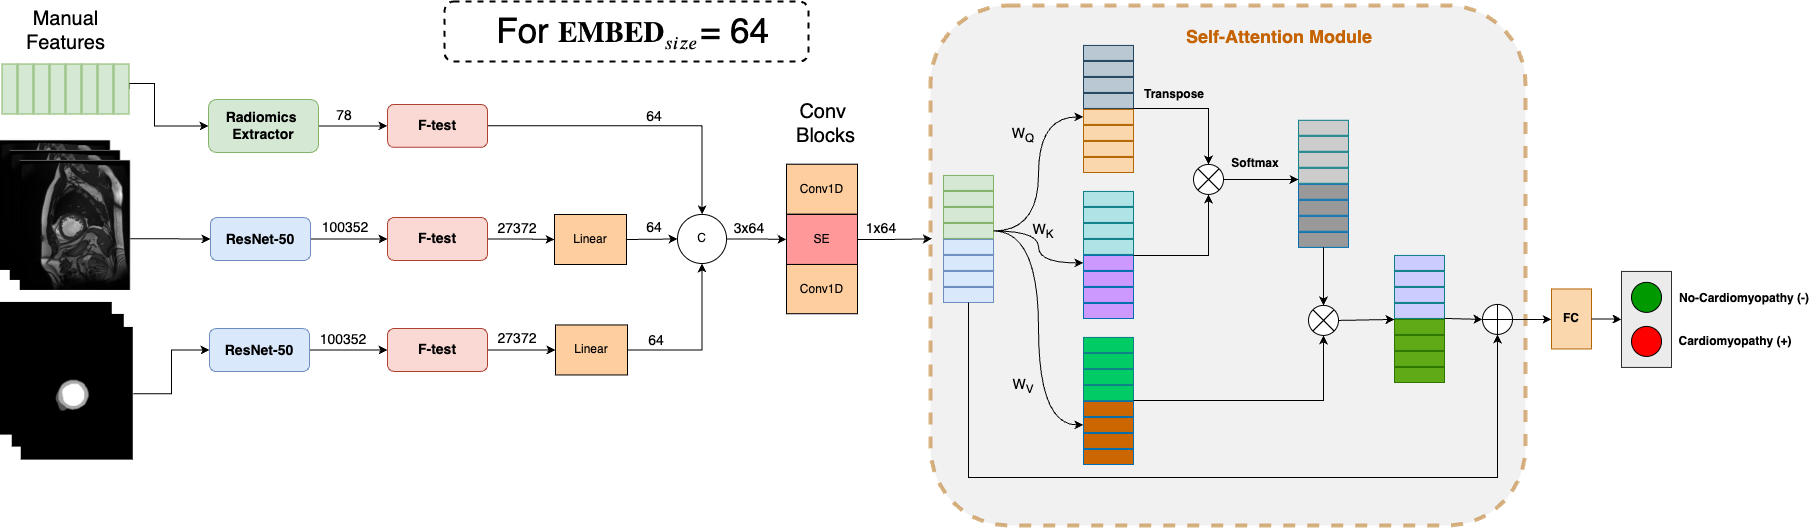
\includegraphics[width=1.02\textwidth]{figures/fig011.png}
    \caption*{Fonte: Autor}
    \label{fig:fig011}
\end{figure}

%---------------------------------------------------------
\section{CONSIDERAÇÕES FINAIS DO CAPÍTULO}
\label{sec:cap4_consideracoes_finais}

Como considerações, destacam-se o uso de base de dados pública, com dados de pacientes incluindo o conjuntos de fatias que identificam a ação de sístole e diástole do coração. É aplicado pré-processamento do qual são extraídas as características radiômicas, características estas que analisam textura, níveis e variações dos tons de cinza incluindo diversas estatísticas como de primeira ordem e o \gls{glcm}. Ainda em fase de pré-processamento é extraída as características profundas oriundas do modelo de visão \textit{ResNet50}, com os pesos treinados na base de dados da \textit{ImageNet}. 

A adaptação inicia ao se adicionar os \textit{embeddings} das máscaras também ao modelo, poder variar o vetor tamanho dos vetores de características, pois no modelo original eram apenas $12$. Os vetores são então extraídos via \textit{F-Test}, concatenados e inseridos no novo bloco convolucional. Este bloco possui um bloco \gls{se} responsável pela atenção seletiva, dando importância aos canais mais pertinentes. Por fim o módulo de autoatenção, confere as relações intrínsecas das transformações anteriores, identificando as características mais determinantes independente de espacialidade e a classificação é apresentada.
\chapter{Resultados E Discussões}
\label{chap:resultados_discussoes}
\vspace{-\baselineskip} %Manter para garantir o espaçamento da biblioteca.


Este capítulo traz informações relacionadas com as ferramentas utilizadas no experimento, como linguagem, bibliotecas utilizadas, entre outros. Assim como, informações sobre o consumo de dados das bases \gls{acdc} e SunnyBrook, fase de pré-processamento, inferência nos modelos implementados, sendo estes, modelo linha de base e derivados, e modelos adaptados. Por fim, são apresentados os resultados considerando as métricas apresentadas na seção \ref{subsec:cap4_metrics} utilizando as bases de dados ACDC e SunnyBrook e cada uma das abordagens: o modelo base e o modelo proposto.

Por fim, este capítulo apresenta os resultados da prova de conceito realizada com os algoritmos desenvolvidos, tanto o modelo base quanto os modelos adaptados, com o intuito de compará-los aos objetivos traçados nesta dissertação. Os testes realizados buscam avaliar a eficiência do algoritmo sob as diversas adaptações discutidas. 

%--------------------------------------------------------
\section{MATERIAIS} 
\label{sec:cap5_materiais}

A Tabela \ref{tab:hardware_software} apresenta as ferramentas que foram utilizadas nesse projeto. Destaca-se que foram utilizadas majoritariamente ferramentas open-source como a linguagem \textit{python}, bibliotecas como \textit{pyradiomics}, \textit{torch}, \textit{numpy}, entre outras. Para registro dos experimentos, foi utilizada a ferramenta CometML\footnote{https://www.comet.com}. No CometML é possível armazenar valores como: erro do lote no treinamento, acurácia do conjuntos de validação no treinamento, métricas resultantes como acurácia, hiperparâmetros como taxa de aprendizado, épocas, etc.
\newline

\begin{table}[hbtp]
    \caption{Fonte: Componentes Utilizados}
    \centering
    \renewcommand{\arraystretch}{1} % default é 1 
    % \begin{tabular}{|>{\centering\arraybackslash}p{2cm}|p{12cm}|}
    \begin{tabular}{|c|c|}
    \hline 
       \textbf{Item} & \textbf{Descrição}\\
    \hline 
       Computador & \textit{Macbook M1 Pro}  \\
    \hline 
       Memória & 16gb  \\
    \hline 
       Versão \textit{Python} & 3.11.0  \\
    \hline 
       Versão \textit{pyradiomics} & 3.0.1 \\
    \hline 
       Versão \textit{torch} & 2.2.1 \\
    \hline 
       Versão \textit{torchvision} & 0.17.1 \\
    \hline 
       Versão \textit{numpy} & 1.26.4 \\
    \hline 
       Versão \textit{scikit-learn} & 1.4.1.post1 \\
    \hline 
       Versão \textit{comet-ml} & 3.47.4 \\
    \hline 
    \end{tabular} 
    \caption*{Fonte: Autor}
    \label{tab:hardware_software}
\end{table}

%--------------------------------------------------------
\section{CENÁRIOS DE TESTE} 
\label{subsec:cap5_dataset}

Este trabalho visou realizar os experimentos em duas bases distintas com imagens de \gls{rmc}, informações a cerca do paciente e rótulos que indicam presença ou não de cardiomiopatia. Testes iniciais foram feitos no conjunto de dados \gls{acdc} que possui $30$ casos de \gls{cmh}, $30$ casos de \gls{cmd} e $90$ casos sem cardiomiopatia, resultando em $60$ casos de cardiomiopatia e $90$ casos sem cardiomiopatia. Da base \gls{acdc} se pretende utilizar apenas as fatias da fase diastólica. O segundo conjunto de dados é o \textit{SunnyBrook}, possuindo imagens na fase diastólica contendo as classes $9$ classes NOR (sem cardiomiopatia) e $12$ HIP (hipertrofia do ventrículo esquerdo).

O modo de operação será o mesmo para ambos os conjuntos de dados com exceção do pré-processamento devido à forma de como o conjunto de dados \textit{SunnyBrook} disponibiliza as máscaras.

Por fim, foram realizados três testes: 1) utilizando o modelo base no conjunto de dados do ACDC; 2) utilizando o modelo adaptado no conjunto de dados do ACDC; 3) utilizando o modelo adaptado no conjunto de dados do SunnyBrook. Todos os testes foram avaliados com as métricas acurácia, precisão, revocação e AUC em ambos os conjuntos de dados.

%--------------------------------------------------------
\section{EXPERIMENTOS MODELO BASE}
\label{sec:cap5_experimentos_base}

Uma prova de conceito foi aplicada ao conjunto de dados \gls{acdc} utilizando o modelo de linha de base para avaliação inicial, avaliação esta também utilizada como linha de base. O modelo base foi implementado seguindo o artigo e sua implementação é conferida na Figura \ref{fig:fig008}. O conjunto de dados para treino é composto por $100$ exames de pacientes, coletando apenas as fatias das imagens da fase diastólica. Características de primeira ordem e \gls{glcm} são extraídas, utilizando a biblioteca \textit{PyRadiomics}, resultando em $\RadiomicFeatures$ valores que compõem as características radiômicas. Para extração das características profundas, foi utilizada uma rede \textit{ResNet50} congelada sem sua última camada linear, responsável pela classificação originalmente de $1000$ classes oriundas do conjunto de dados \textit{ImageNet}, obtendo como resultado final um vetor com $\DeepFeatures$ características profundas.

% O \textit{F-Test} é utilizado como um seletor de características inicial, aplicado tanto nas características radiômicas quanto nas profundas, reduzindo garantindo que os vetores possuam m profundas, com um total de $\text{EMBED}_{size}$ igual a $12$  no modelo base. As características resultantes do \textit{F-Test}, agora com tamanhos agora iguais, são concatenadas e enviadas ao módulo de autoatenção e os resultados armazenados.

Neste experimento foi treinado o modelo utilizando como função objetivo a entropia cruzada binária, taxa de aprendizado de $\LR$, otimizador \textit{Adam}, tamanho de lote $\Batch$ e o treinamento se deu com aproximadamente $\Epochs$ épocas, em que foi verificado que o erro se torna estável em tempo de treinamento. Também foi empregada a estratégia de aleatorizar as entradas no modelo em tempo de treinamento. Ao vetor resultante da saída do modelo é aplicada a função sigmoide, conforme Equação \ref{eq:sigmoide}, função esta que limita os valores de sua entrada entre 0 e 1. Para fins de classificação, foi considerado valores maiores que $0,5$ são considerados com cardiomiopatia e menores ou iguais a $0,5$ são considerados sem cardiomiopatia.

\begin{equation}
\textit{sigmoide}(x) = \frac{1}{1 + e^{-x}}
\label{eq:sigmoide}
\end{equation}

% --------------------------------------------------------
\section{EXPERIMENTOS MODELOS PROPOSTO}
\label{sec:cap5_experimentos_adaptados}

Os modelos adaptados refletem os experimentos desmembrados do modelo base, adaptações estas com a finalidade de verificar se mudanças, seja nos hiperparâmetros, seja em partes da arquitetura, podem trazer resultados promissores em relação aos resultados base. As mudanças podem ser elencadas em: 

\begin{enumerate}

\item Mudanças do $\text{EMBED}_{size}$ em que foram testados os valores $[24, 48, 64]$ na tentativa de preservar mais informações originais;

\item No caso das versões adaptadas, também há a adição do consumo das respectivas máscaras que são futuramente concatenadas as características radiômicas e profundas;

\item A concatenação é feita de forma diferente, assumindo por exemplo o valor de $\text{EMBED}_{size}$ igual a $12$, na versão original tem-se como resultado $1\times24$ porém na versão adaptada essa concatenação é feita na primeira dimensão, resultando neste exemplo em $2\times12$. Isto se dá por apresentar um novo bloco ao modelo original o bloco convolucional, composto de convolução e blocos \gls{se}.

\end{enumerate}


A parte restante da arquitetura segue de acordo com a original, exceto que também podemos variar $N$ vezes o bloco de autoatenção, ou seja, sua saída volta sendo sua entrada $N$ vezes e este valor de $N$ também pode ser considerado como um dos hiperparâmetros do experimento. Os valores de $N$ utilizados foram $[1, 2, 4, 6]$. Estas mudanças não mudam a estrutura da arquitetura inicial fazendo com que o módulo autoatenção seja executado $N$ vezes conforme trabalho de \cite{vaswaniAttentionAllYou2023} e pode ser visualizada na Figura \ref{fig:fig030}.

\begin{figure}[H]
    \centering
    \captionsetup{width=0.98\textwidth, justification=justified}
    \caption{Representação esquemática da recorrência do Módulo de Autoatenção. O diagrama ilustra o processamento recursivo na arquitetura proposta, recursividade esta que permite que as características aprendidas sejam refinadas ao longo de múltiplas iterações, aumentando a capacidade do modelo de capturar dependências complexas nos dados.
    }
    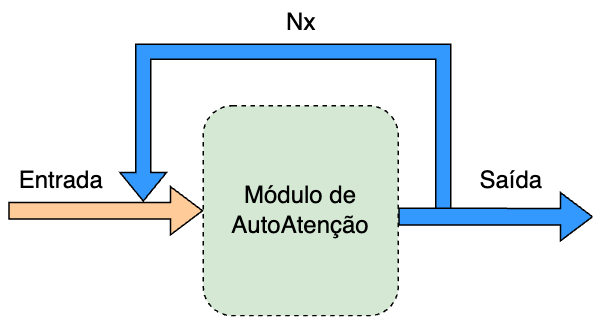
\includegraphics[width=0.7\textwidth]{figures/fig030.png}
    \caption*{Fonte: Autor}
    \label{fig:fig030}
\end{figure}


% Posso elencar novamente de forma sucinta os hiperparamentros aqui: EMBED_SIZE, N attention blocks, imagems de mascara e nova forma de concatenar. 


%--------------------------------------------------------
% \section{Cronograma}
% \label{sec:cronograma}

% O cronograma proposto das atividades segue na Figura \ref{fig:fig014}. Os itens em azul são atividades concluídas como: disciplinas, revisão bibliográfica, refinamento do tema, testes iniciais, etc. Itens em rosa são atividades em andamento como: implementação de modelos de comparação e escrita da dissertação. Atividades em amarelo são atividades planejadas como: análise de resultados, escrita da dissertação e escrita de artigos.

% \begin{figure}[htbp]
%     \centering
%     \caption{Cronograma planejado}
%     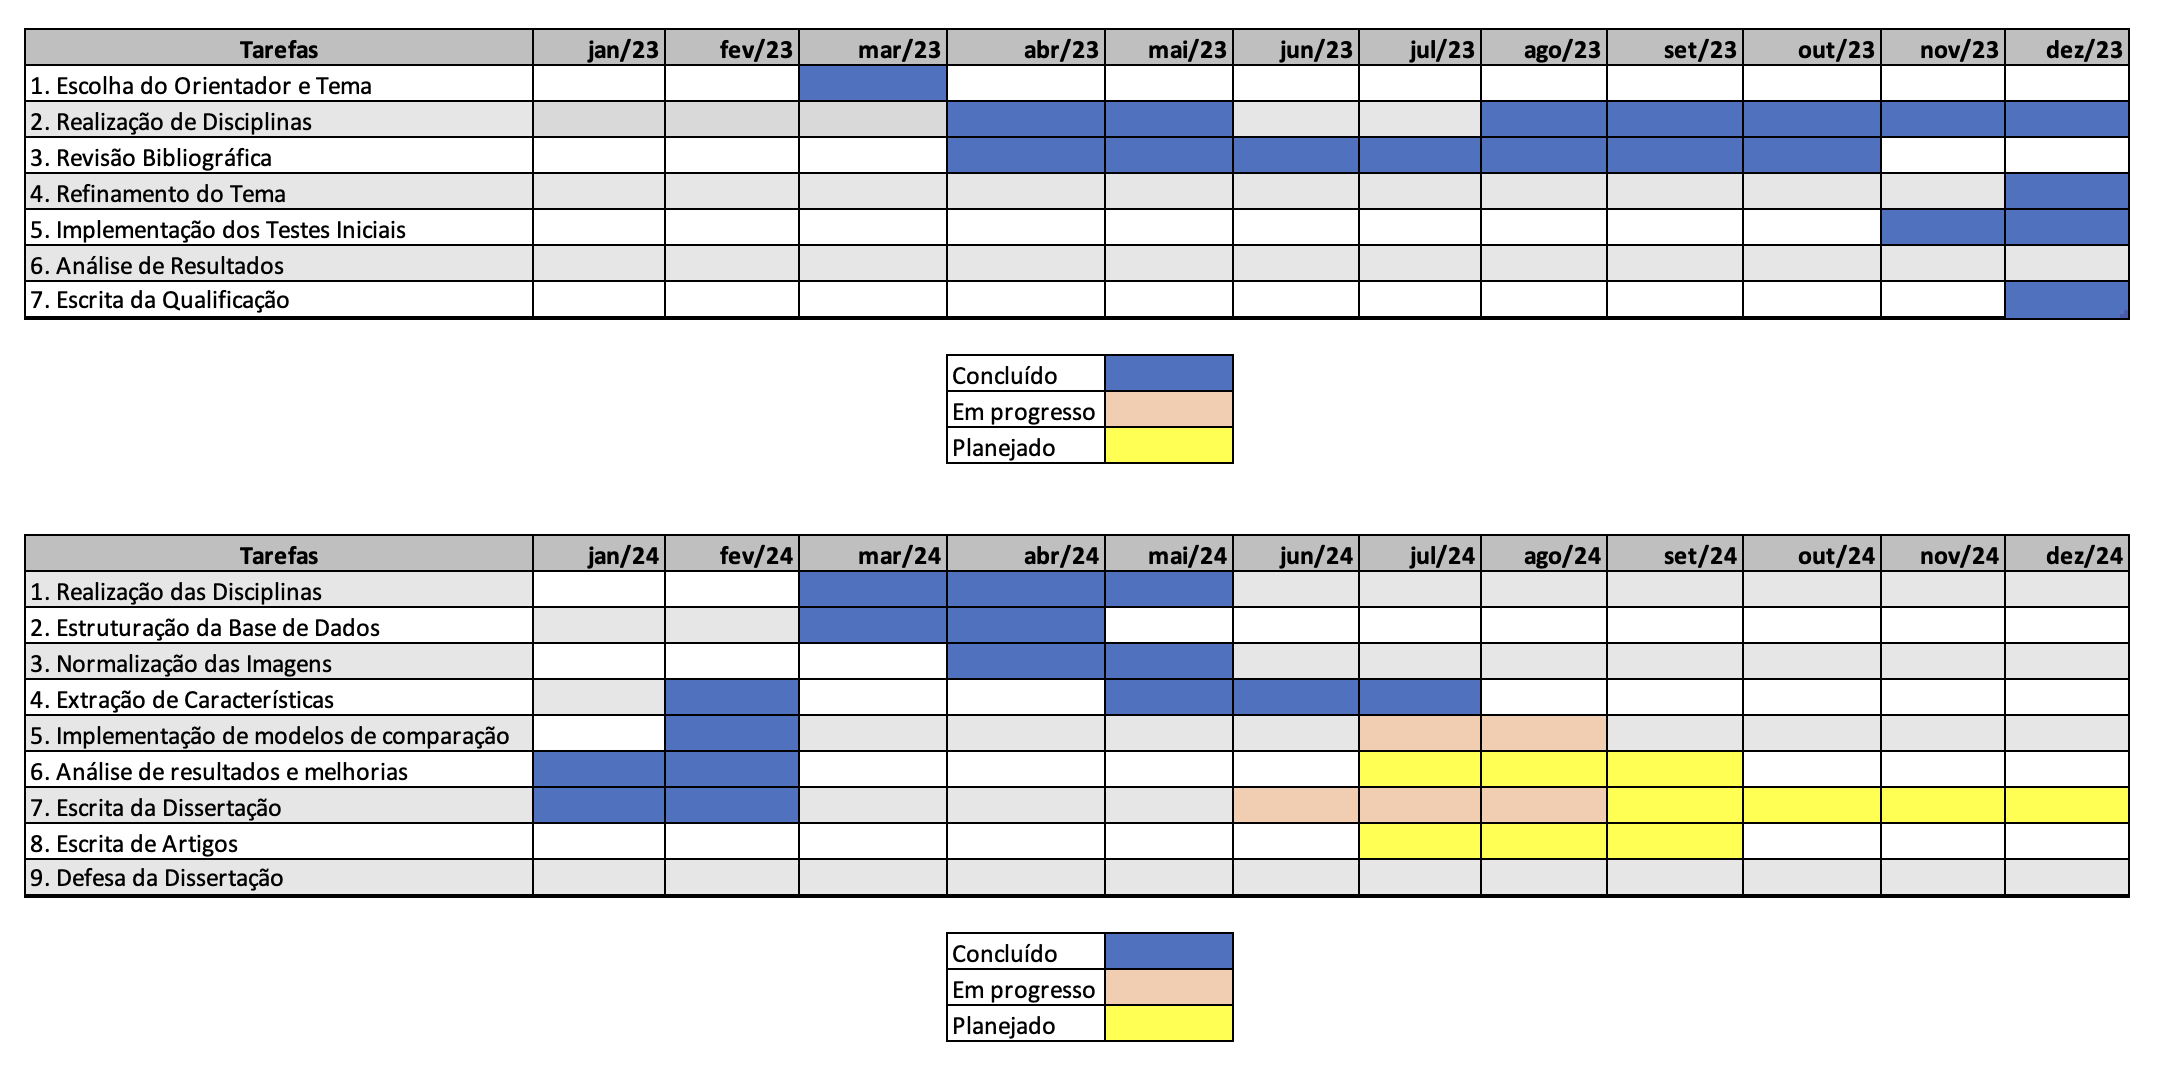
\includegraphics[width=1\textwidth]{figures/fig014.png}
%     \caption*{Fonte: Autor}
%     \label{fig:fig014}
% \end{figure}

%--------------------------------------------------------
\section{RESULTADOS ACDC}
\label{sec:resultados_acdc}

O conjunto de dados \gls{acdc} foi a referência inicial, principalmente para a coleta dos resultados com o modelo base. Este conjunto de dados público já se encontra separado com $100$ exames para treino e $50$ para testes. A Figura \ref{fig:fig018} e \ref{fig:fig019} são exemplos respectivamente, de imagens de \gls{dcm} e \gls{hcm} capturadas na diástole com suas respectivas máscaras, lembrando que ambas representam cardiomiopatia hipertrófica. Na Figura \ref{fig:fig020} temos a imagem de coração em estado sem anomalia (\gls{nor}) e sua respectiva máscara. As imagens demonstradas fazem parte do conjunto real de treinamento.

\begin{figure}[h!]
    \centering
    \captionsetup{width=0.98\textwidth, justification=justified}
    \caption{Captura Diastólica CMD}
    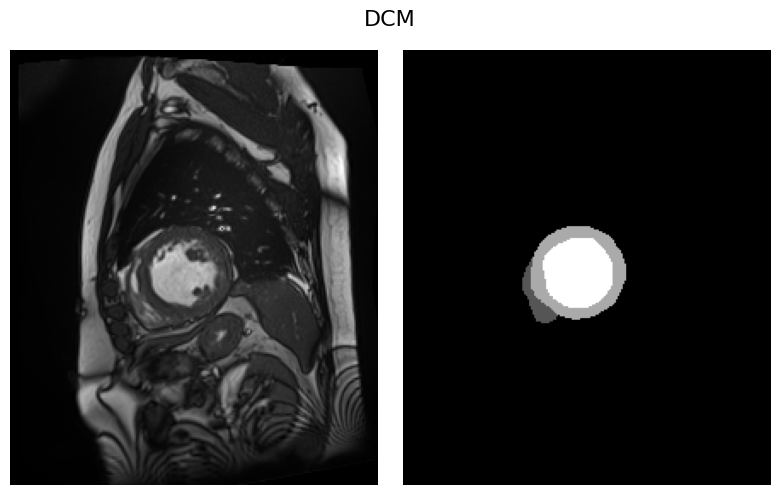
\includegraphics[width=0.65\textwidth]{figures/fig018.png}
    \caption*{Fonte: Autor}
    \label{fig:fig018}
\end{figure}

\begin{figure}[h!]
    \centering
    \captionsetup{width=0.98\textwidth, justification=justified}
    \caption{Captura Diastólica de CMH}
    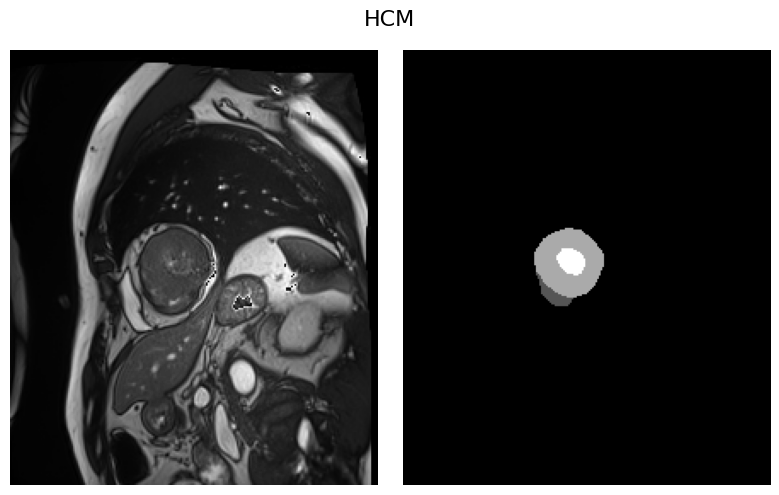
\includegraphics[width=0.65\textwidth]{figures/fig019.png}
    \caption*{Fonte: Autor}
    \label{fig:fig019}
\end{figure}

\begin{figure}[h!]
    \centering
    \captionsetup{width=0.98\textwidth, justification=justified}
    \caption{Captura Diastólica NOR}
    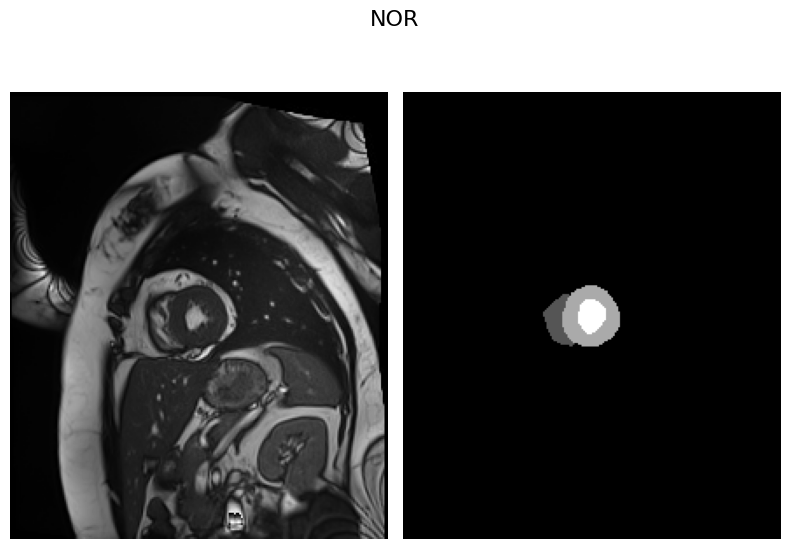
\includegraphics[width=0.65\textwidth]{figures/fig020.png}
    \caption*{Fonte: Autor}
    \label{fig:fig020}
\end{figure}

%--------------------------------------------------------
\subsection{Resultados dos Modelos Base - ACDC}
\label{subsec:resultados_acdc_base}

Com os dados pré-processados e previamente armazenados, o treinamento é efetuado com os vetores radiômicos e profundos. As métricas parciais foram sendo salvas em tempo de treinamento. Para o modelo base os hiperparâmetros são: $\text{EMBED}_{size}$ igual a $12$, $N$ igual 1, ou seja, apenas um bloco de auto atenção, dimensão de concatenação $1$, taxa de aprendizado $\LR$, otimizador \gls{adam}, tamanho de lote $\Batch$ e aproximadamente $\Epochs$ épocas. Uma vez treinado, foi feita a inferência no conjunto de dados de teste, aplicando a função sigmoide e definindo $0,5$ como o valor de corte onde os valores acima deste limite são classificados como \gls{car} e os demais como sem cardiomiopatia. 

As métricas resultantes podem ser conferidas na Tabela \ref{tab:metrics}. A matriz de confusão é apresentada na Figura \ref{fig:fig016} e um gráfico ilustrando da \gls{roc} é apresentado na Figura \ref{fig:fig017}.
\newline

\begin{table}[h!]
    \centering
    \caption{Métricas do Experimento - Modelo Base}
    \renewcommand{\arraystretch}{1} % default é 1 
    \begin{tabular}{|c|c|}
    \hline 
          \textbf{Métrica} & \textbf{Valor} \\ 
    \hline 
        Acurácia & 0.58 \\ 
    \hline 
        Precisão & 0.47 \\ 
    \hline 
        Revocação & 0.45 \\ 
    \hline 
        AUC & 0.55 \\ 
    \hline 
    \end{tabular} 
    \caption*{Fonte: Autor}
    \label{tab:metrics}
\end{table}

\begin{figure}[h!]
    \centering
    \captionsetup{width=0.98\textwidth, justification=justified}
    \caption{Matriz de confusão do modelo base, apresentando os resultados da classificação binária. Observa-se 20 verdadeiros negativos, 9 verdadeiros positivos, 10 falsos positivos e 11 falsos negativos, totalizando 50 amostras com acurácia de 58\%.
    }
    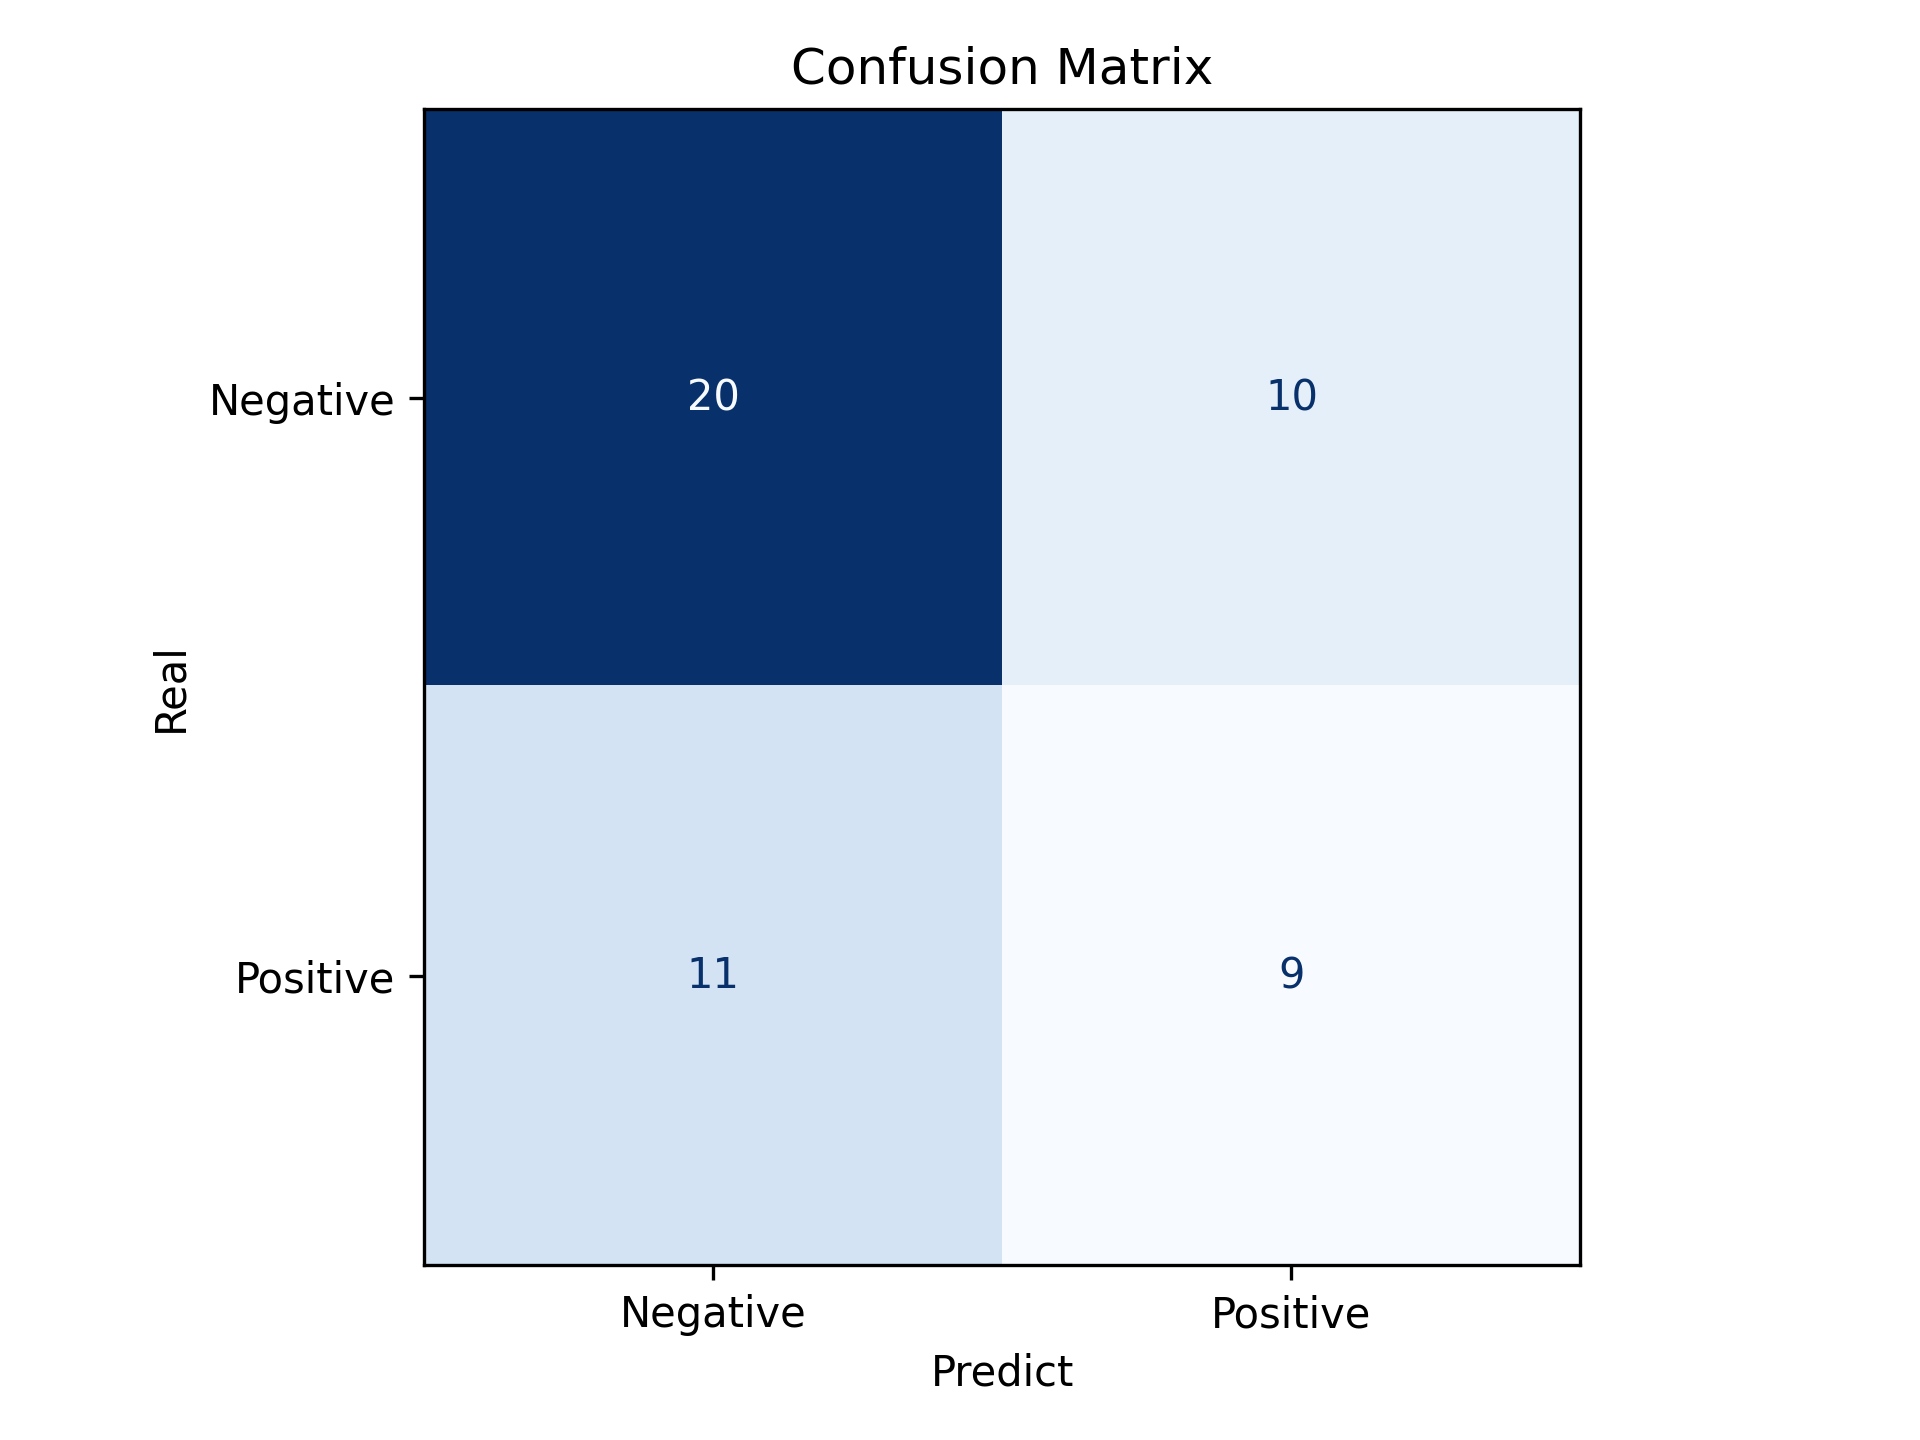
\includegraphics[width=0.55\textwidth]{figures/fig016.png}
    \caption*{Fonte: Autor}
    \label{fig:fig016}
\end{figure}

\begin{figure}[h!]
    \centering
    \captionsetup{width=0.98\textwidth, justification=justified}
    \caption{Curva \gls{roc} obtida pelo modelo proposto, ilustrando a relação entre a taxa de verdadeiros positivos (sensibilidade) e a taxa de falsos positivos.
    }
    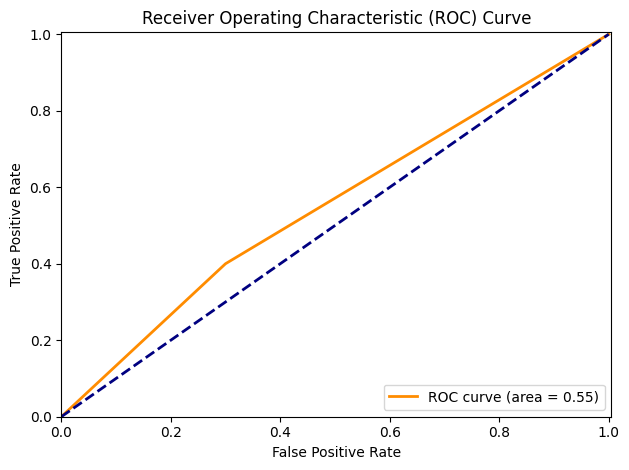
\includegraphics[width=0.75\textwidth]{figures/fig017.png}
    \caption*{Fonte: Autor}
    \label{fig:fig017}
\end{figure}


Para o registro dos resultados foi utilizada a ferramenta \textit{CometML}. O \textit{CometML} pode registrar, em tempo de execução, informações como erro por lote, erro por época, acurácia de validação, etc, podem ser armazenados enquanto o processo de treinamento é executado. Por fim métricas como acurácia e matriz de confusão podem ser armazenadas também. O serviço é acessado  por uma \gls{api} externa. As Figuras \ref{fig:fig028} e \ref{fig:fig029} demonstram respectivamente os painéis adaptáveis com alguns dos hiperparâmetros e métricas coletadas durante e ao terminar o treino. É possível notar que o modelo se sobre-ajusta nos dados de treino, com acurácia $1$, predizendo corretamente todos os valores porém, nos dados de teste a assertividade cai drasticamente para $0,58$. Também é possível notar que após $2500$ passos no treinamento, o erro de treinamento estabiliza e os demais processamentos não se fazem necessários.

\begin{figure}[h!]
    \centering
    \captionsetup{width=0.98\textwidth, justification=justified}
    \caption{Painéis adaptáveis gerados pela plataforma \textit{CometML} durante o treinamento do modelo. A visualização superior apresenta a evolução da função de perda (loss) ao longo dos passos de treinamento, com picos iniciais que se estabilizam no decorrer do treino. Os painéis inferiores mostram as métricas finais obtidas: acurácia de treinamento de 100\% e acurácia de teste de 58\% (valor 0.58)., evidenciando um possível sobreajuste do modelo.  
    }
    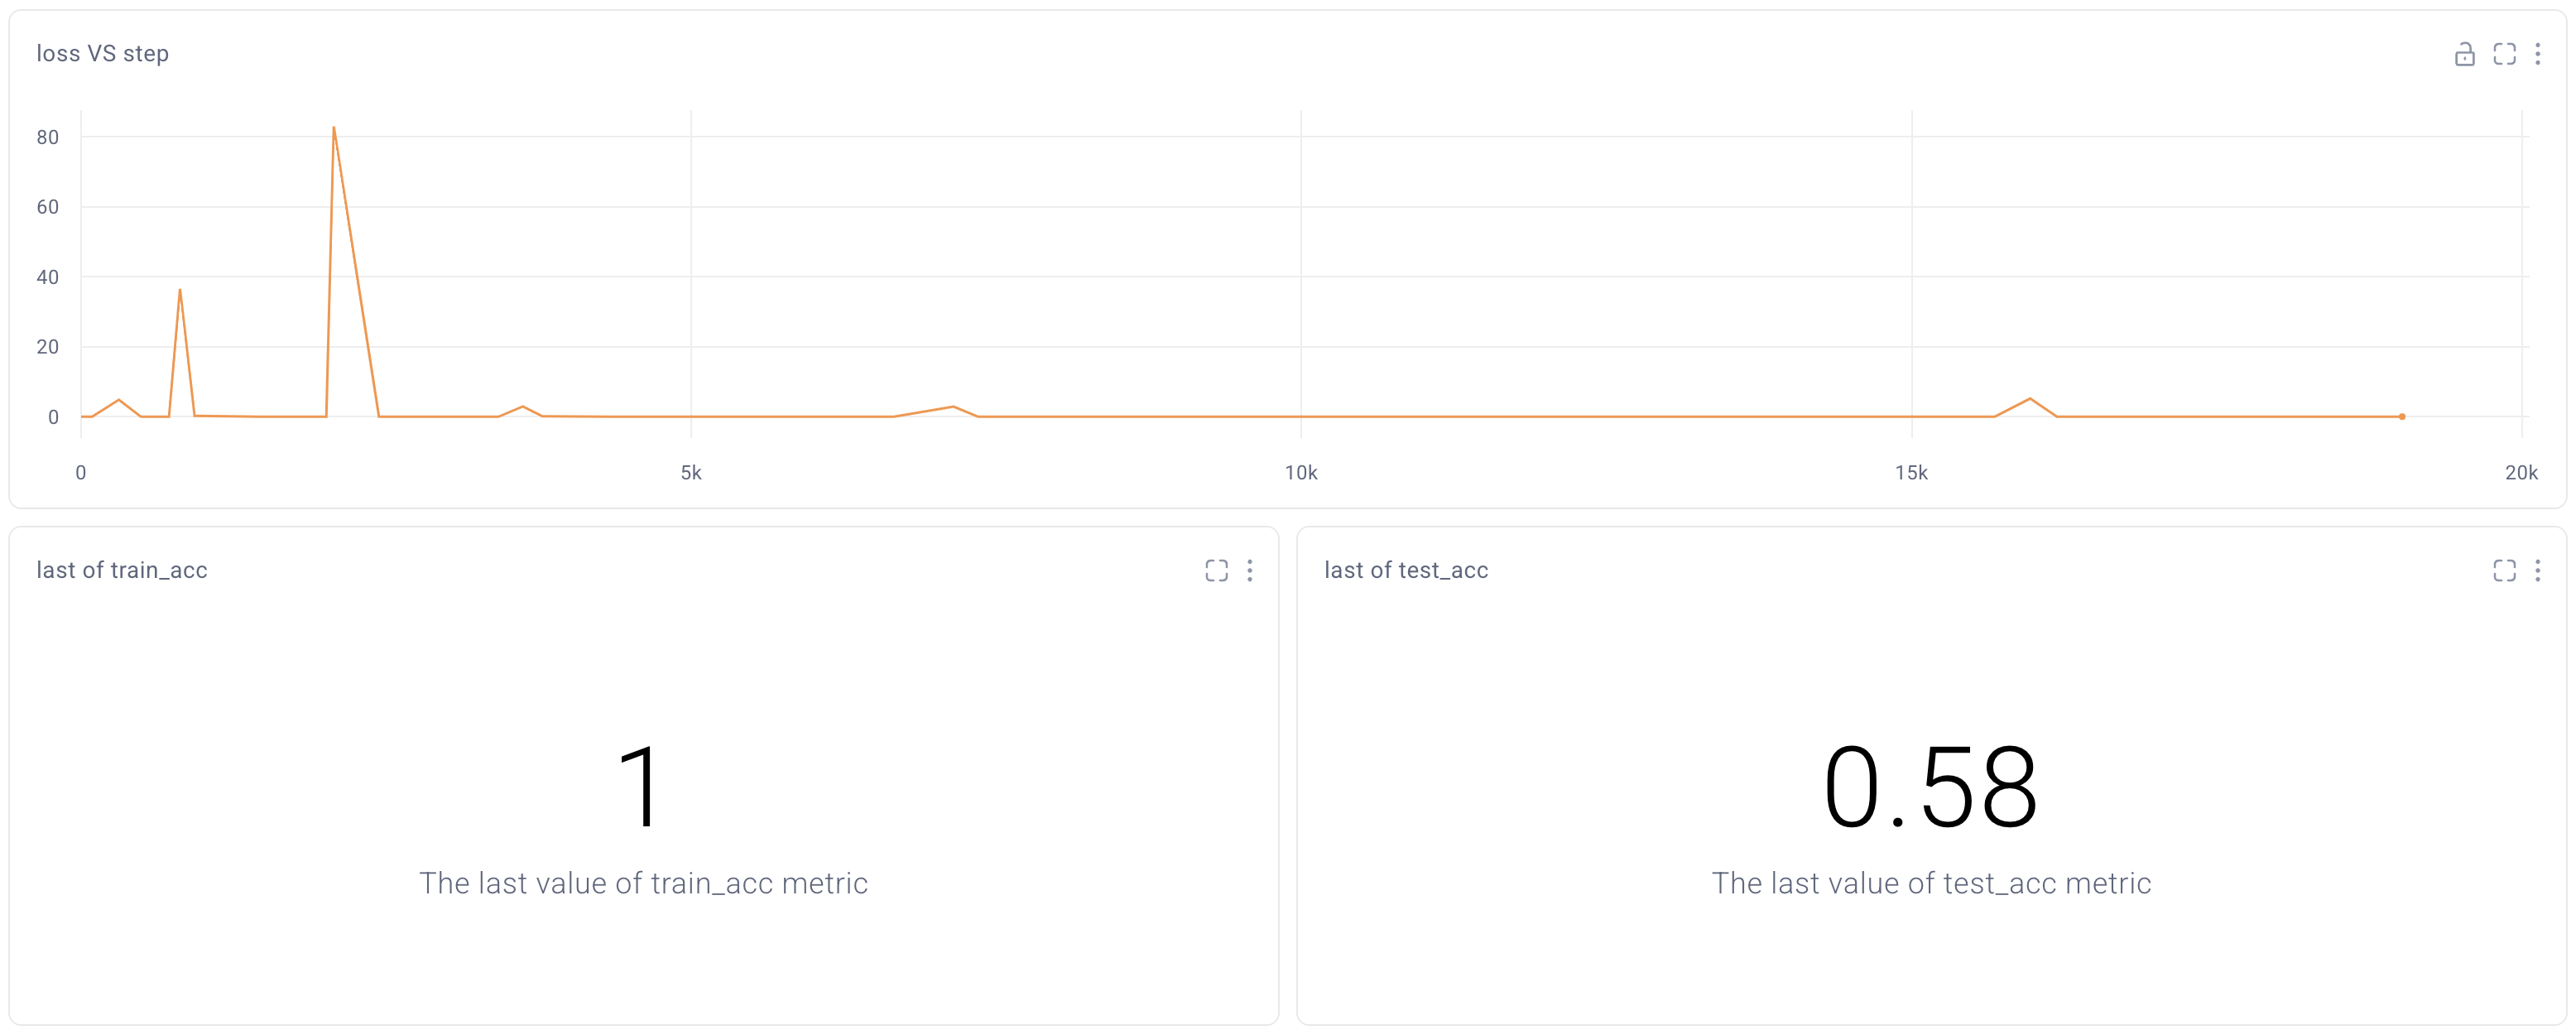
\includegraphics[width=1\textwidth]{figures/fig028.png}
    \caption*{Fonte: Autor}
    \label{fig:fig028}
\end{figure}


\begin{figure}[h!]
    \centering
    \captionsetup{width=0.98\textwidth, justification=justified}
    \caption{Valores Coletados no Treino gerados pela plataforma \textit{CometML} incluindo: função de perda (loss), acurácia de treino, e teste.}
    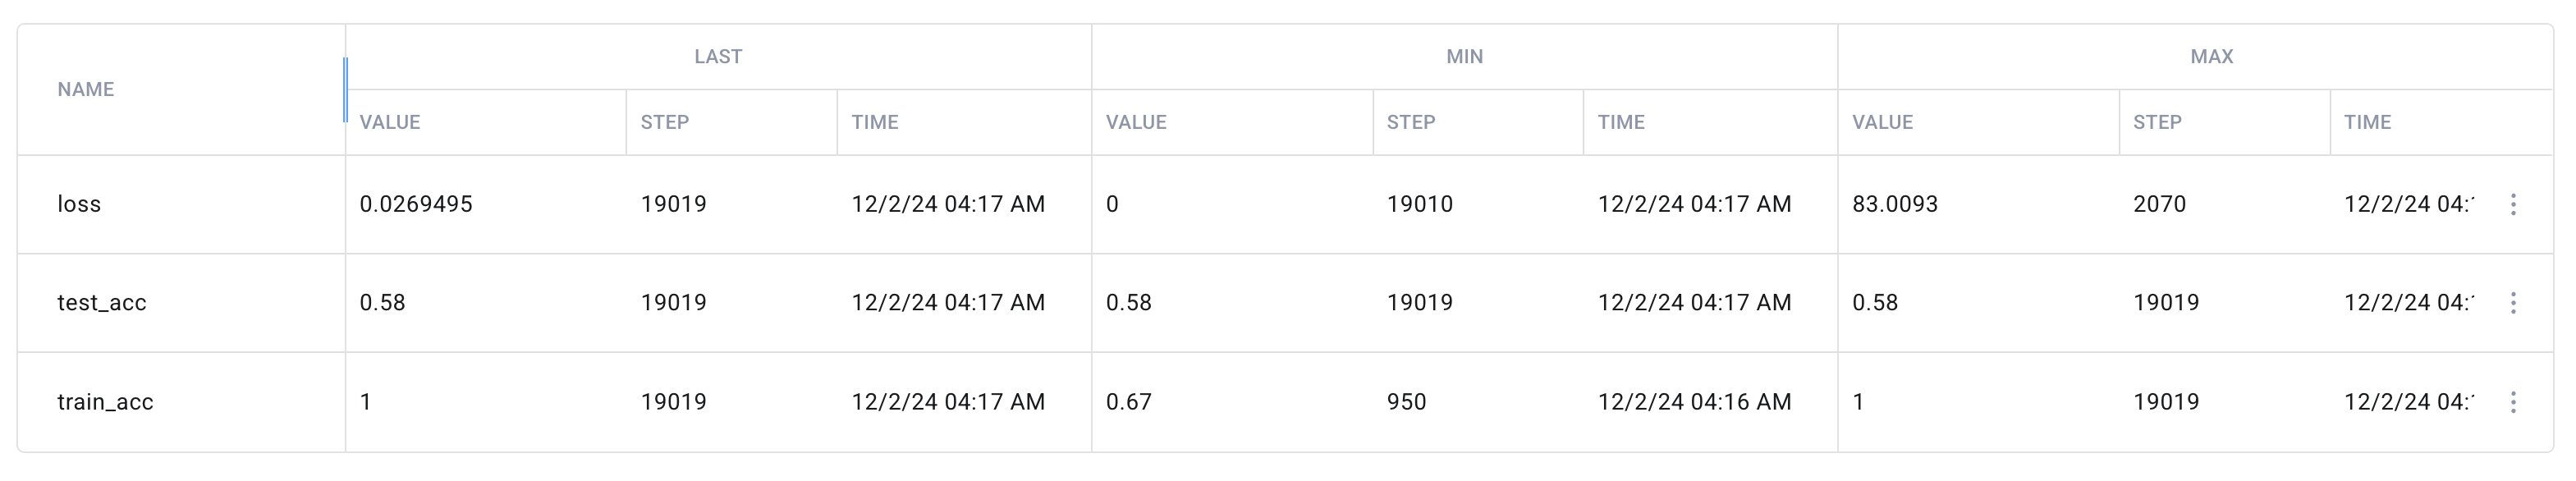
\includegraphics[width=1\textwidth]{figures/fig029.png}
    \caption*{Fonte: Autor}
    \label{fig:fig029}
\end{figure}


%--------------------------------------------------------
\subsection{Resultados dos Modelos Adaptados - ACDC}
\label{subsec:resultados_acdc_adaptado}

Para as versões adaptadas, se buscou mudar os hiperparâmetros e até mesmo a arquitetura do modelo com o intuito comparar os resultados com a versão base. Os primeiros experimentos foram aplicados variando o $\text{EMBED}_{size}$, também foi aplicado $N$ vezes o bloco de autoatenção ao invés de uma única vez. Os experimentos foram executados gerando a combinatória destes hiperparâmetros para cobrir o máximo de cenários possíveis dentro da metodologia.

Também foi introduzido, nas versões adaptadas, um módulo convolucional, que antecede o módulo de autoatenção. Este módulo convolucional é composto de três blocos: uma camada convolucional 1D, um bloco \gls{se} e outro bloco convolucional 1D. Com a possibilidade de se ter que adicionar opcionalmente um terceiro vetor de características, sendo este a máscara, foi possível identificar relações intrínsecas entre mais este vetor. A concatenação agora na primeira dimensão faz cada vetor de característica se tornar um canal. 

No módulo convolucional, uma primeira camada de convolução 1D aumenta o número de canais para $16$, ou seja, $16$ filtros são aplicado para extração de informação espacial. O bloco \gls{se} representa a camada de atenção seletiva que dá importância aos canais mais importantes, identificando a relevância de cada canal e finaliza escalando os canais na entrada original com um valor escalar otimizado em tempo de treinamento. Detalhes podem ser vistos na Figura \ref{fig:fig031}. O bloco \gls{se} neste projeto é adaptado para ser 1D, diferente do trabalho original que visa sua aplicação em modelos de visão computacional já consolidados. O valor de $r$ no bloco \gls{se} ficou fixo em $16$, os autores do trabalho original fazem testes empíricos e confirmam que o valor de $16$ é o que traz melhores resultados.

\begin{figure}[h!]
    \centering
    \captionsetup{width=0.98\textwidth, justification=justified}
    \caption{Composição Bloco SE. O diagrama ilustra o fluxo de processamento em três etapas principais: Squeeze (compressão), que reduz a dimensionalidade espacial através de Global Pooling; Excitation (excitação), composta por duas camadas totalmente conectadas (FC) com funções de ativação ReLU e Sigmoid; e Scaling (escalonamento), que recalibra os mapas de características originais. Este mecanismo permite que a rede aprenda interdependências entre canais e atribua pesos adaptativos para realçar características relevantes.
    }
    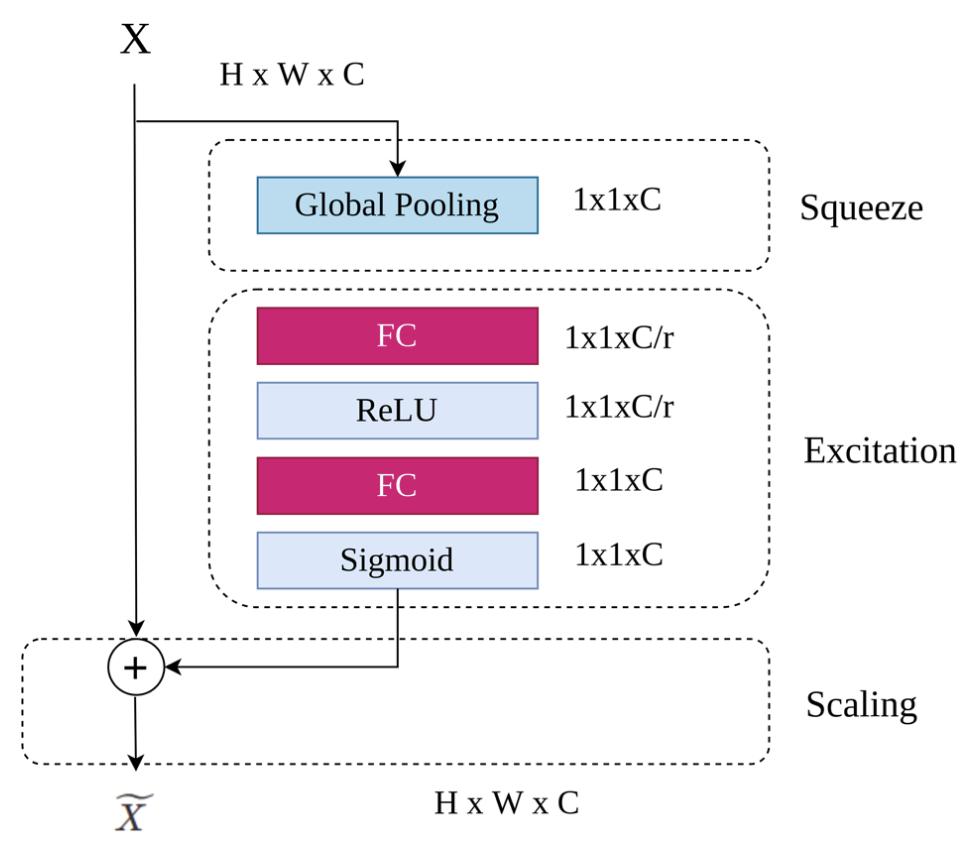
\includegraphics[width=0.7\textwidth]{figures/fig031.png}
    \caption*{Fonte: Adaptado de \cite{lafraxoSEDARUnetSqueezeexcitationDilated2024}}
    \label{fig:fig031}
\end{figure}


A Tabela \ref{tab:metrics_acdc_orig} apresenta o conjunto de experimentos na versão original e versões adaptadas. A Tabela \ref{tab:metrics_acdc_orig_mask} demonstra os experimentos adicionando a máscara como um terceiro vetor de características. A Tabela \ref{tab:metrics_acdc_se} apresenta a adição de blocos convolucionais e  \gls{se}. Alguns pontos podem ser notados no experimento, o treinamento quase sempre sofre sobre-ajuste ficando muito próximo de 100\% de assertividade, isso pode se justificado dado o fato de haver poucos exemplares para treinamento. Outro ponto notado é que quanto maior o tamanho do vetor de características (Emb) melhor costuma ser o resultado. Quantidades maiores no número de blocos de autoatenção (N\_Attn) também melhoram os resultados, exceto no caso em que são configurados em $6$. A justificativa se deve ao fato de tornar o modelo mais complexo se comparados a quantidade de dados limitadas para treino, prejudicando a sua capacidade de generalização. Os melhores resultados são conferidos nas versões que adicionam o bloco \gls{se} e com quatro blocos de autoatenção, sendo que o melhor experimento obteve $78\%$ de assertividade.


\begin{table}[htbp]
\centering
\caption{Métricas ACDC - Adaptação do Modelo Original
\newline Negrito representa o modelo base}
\begin{tabular}{lcccccc}
\toprule
\textbf{Emb} & \textbf{N\_Attn} & \textbf{Acc} & \textbf{Precision} & \textbf{Recall} & \textbf{F1} & \textbf{AUC} \\
\midrule
\textbf{24} & \textbf{1} & \textbf{0,58} & \textbf{0,47} & \textbf{0,45} & \textbf{0,46} & \textbf{0,55} \\
24 & 2 & 0,58 & 0,48 & 0,60 & 0,53 & 0,58 \\
24 & 4 & 0,54 & 0,44 & 0,55 & 0,49 & 0,54 \\
24 & 6 & 0,50 & 0,41 & 0,55 & 0,47 & 0,51 \\
\hline
48 & 1 & 0,62 & 0,52 & 0,55 & 0,54 & 0,61 \\
48 & 2 & 0,64 & 0,54 & 0,65 & 0,59 & 0,64 \\
48 & 4 & 0,66 & 0,56 & 0,70 & 0,62 & 0,67 \\
48 & 6 & 0,64 & 0,54 & 0,70 & 0,61 & 0,65 \\
\hline
64 & 1 & 0,62 & 0,52 & 0,65 & 0,58 & 0,62 \\
64 & 2 & 0,64 & 0,54 & 0,70 & 0,61 & 0,65 \\
64 & 4 & 0,66 & 0,57 & 0,65 & 0,60 & 0,66 \\
64 & 6 & 0,64 & 0,54 & 0,65 & 0,59 & 0,64 \\
\bottomrule
\end{tabular}
\caption*{Fonte: Autor}
\label{tab:metrics_acdc_orig}
\end{table}


\begin{table}[htbp]
\centering
\caption{Métricas ACDC - Adaptação do Modelo Original + Máscaras
\newline Negrito representa maior assertividade}
\begin{tabular}{lcccccc}
\toprule
\textbf{Emb} & \textbf{N\_Attn} & \textbf{Acc} & \textbf{Precision} & \textbf{Recall} & \textbf{F1} & \textbf{AUC} \\
\midrule
24 & 1 & 0,44 & 0,35 & 0,45 & 0,39 & 0,44 \\
24 & 2 & 0,46 & 0,38 & 0,55 & 0,45 & 0,48 \\
24 & 4 & 0,48 & 0,36 & 0,40 & 0,38 & 0,47 \\
24 & 6 & 0,48 & 0,38 & 0,45 & 0,41 & 0,47 \\
\hline
48 & 1 & 0,52 & 0,44 & 0,70 & 0,54 & 0,55 \\
48 & 2 & 0,58 & 0,48 & 0,55 & 0,51 & 0,57 \\
48 & 4 & 0,62 & 0,52 & 0,60 & 0,56 & 0,62 \\
48 & 6 & 0,60 & 0,50 & 0,50 & 0,50 & 0,58 \\
\hline
64 & 1 & 0,58 & 0,48 & 0,60 & 0,53 & 0,58 \\
64 & 2 & 0,56 & 0,45 & 0,50 & 0,48 & 0,55 \\
\textbf{64} & \textbf{4} & \textbf{0,64} & \textbf{0,54} & \textbf{0,65} & \textbf{0,59} & \textbf{0,64} \\
64 & 6 & 0,62 & 0,53 & 0,45 & 0,49 & 0,59 \\
\bottomrule
\end{tabular}
\caption*{Fonte: Autor}
\label{tab:metrics_acdc_orig_mask}
\end{table}


\begin{table}[htbp]
\centering
\caption{Métricas ACDC - Modelos Adaptados - Blocos Conv. + SE
\newline Negrito representa maior assertividade}
\begin{tabular}{lcccccc}
\toprule
\textbf{Emb} & \textbf{N\_Attn} & \textbf{Acc} & \textbf{Precision} & \textbf{Recall} & \textbf{F1} & \textbf{AUC} \\
\midrule
24 & 1 & 0,66 & 0,56 & 0,70 & 0,62 & 0,67 \\
24 & 2 & 0,68 & 0,58 & 0,75 & 0,65 & 0,69 \\
24 & 4 & 0,70 & 0,59 & 0,80 & 0,68 & 0,72 \\
24 & 6 & 0,68 & 0,59 & 0,65 & 0,62 & 0,67 \\
\hline
48 & 1 & 0,70 & 0,58 & 0,90 & 0,71 & 0,73 \\
48 & 2 & 0,70 & 0,62 & 0,65 & 0,63 & 0,69 \\
48 & 4 & 0,74 & 0,65 & 0,75 & 0,70 & 0,74 \\
48 & 6 & 0,70 & 0,60 & 0,75 & 0,67 & 0,71 \\
\hline
64 & 1 & 0,64 & 0,54 & 0,65 & 0,59 & 0,64 \\
64 & 2 & 0,72 & 0,64 & 0,70 & 0,67 & 0,72 \\
\textbf{64} & \textbf{4} & \textbf{0,78} & \textbf{0,76} & 0,65 & 0,70 & 0,76 \\
64 & 6 & 0,76 & 0,65 & \textbf{0,85} & \textbf{0,74} & \textbf{0,77} \\
\bottomrule
\end{tabular}
\caption*{Fonte: Autor}
\label{tab:metrics_acdc_se}
\end{table}


% \begin{figure}[h!]
%     \centering
%     \caption{Modelos c/ Bloco SE e sua Acurácia - \textit{CometML}}
%     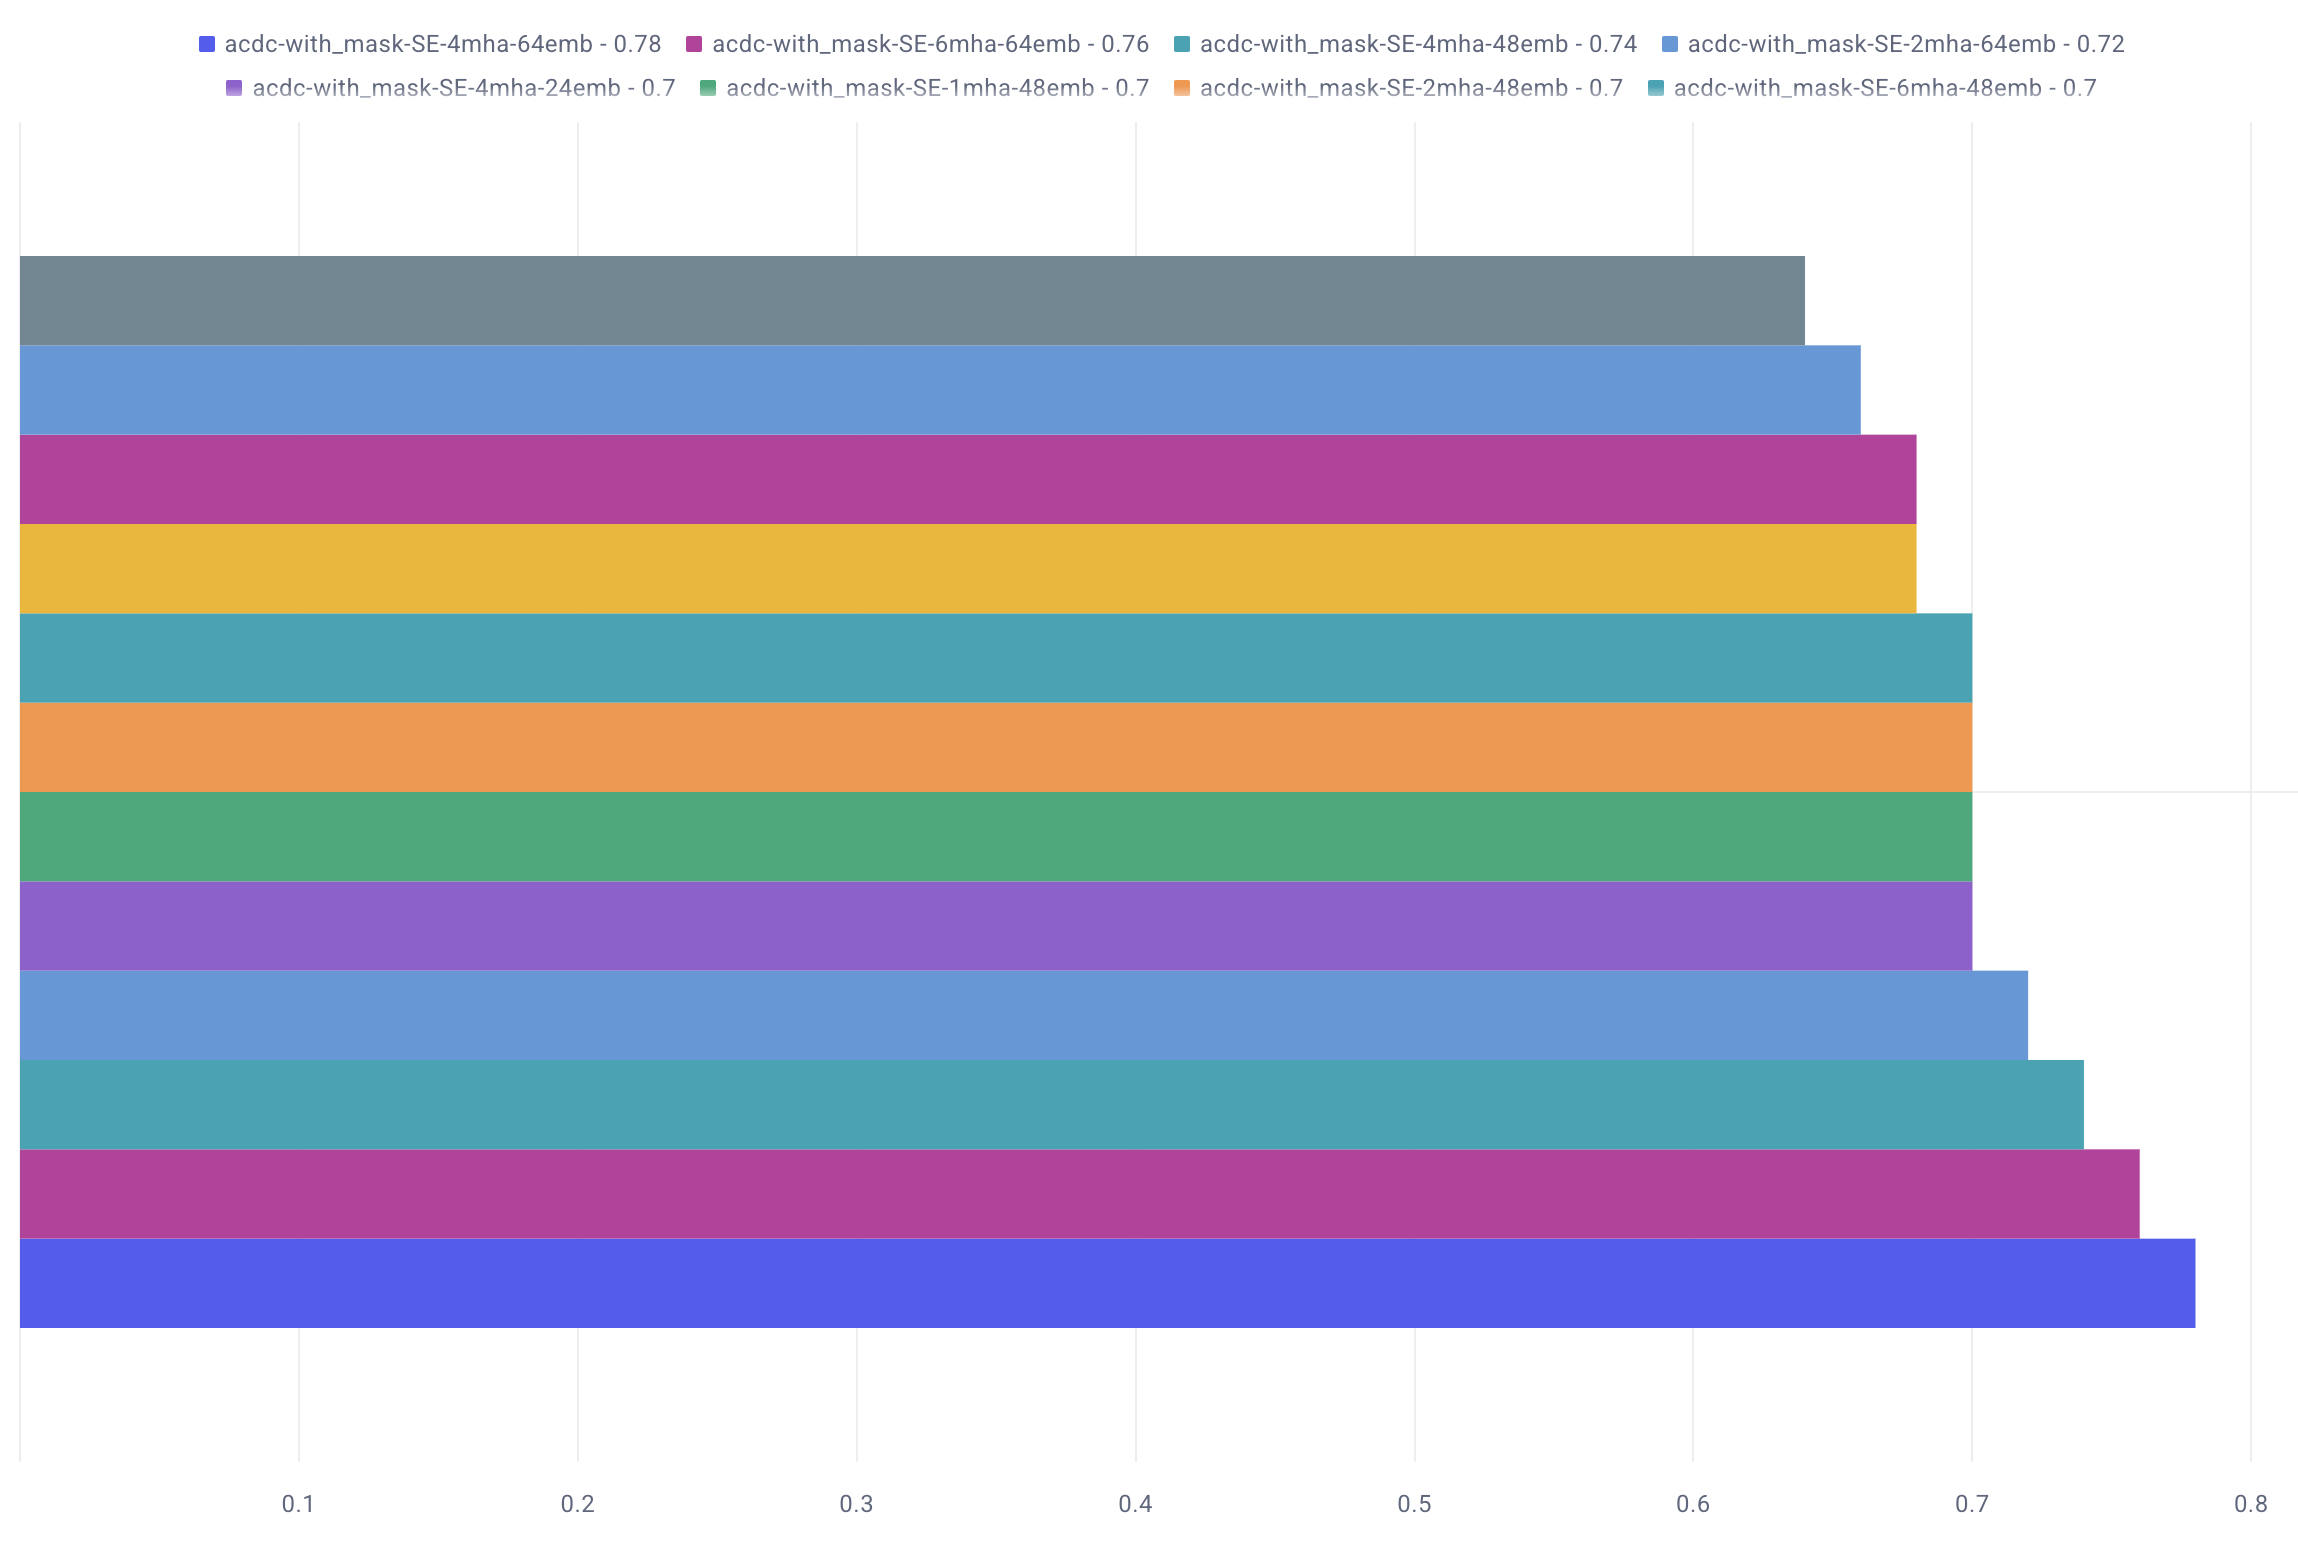
\includegraphics[width=1\textwidth]{figures/fig032.png}
%     \caption*{Fonte: Autor}
%     \label{fig:fig032}
% \end{figure}

%--------------------------------------------------------
\subsection{Resultados dos Modelos Adaptados - \textit{SunnyBrook}}
\label{subsec:resultados_sunny_adaptado}

Os experimentos no conjunto de dados \textit{SunnyBrook} foram os mesmos aplicados ao conjunto de dados \gls{acdc}. No conjunto de dados \textit{SunnyBrook}, houve uma etapa extra de pré-processamento para gerar as máscaras. Foi necessário interpolar os valores de um arquivo de texto que vem anexo com os dados. A máscara também é composta apenas pela região de interesse com valores entre 0 e 1.

Como o \textit{SunnyBrook} tem poucos dados, apenas $45$, sendo $30$ para treino e $15$ para teste e removendo as classes de infarto (IC e IC-I), sobram $21$ registros sendo $13$ para treino e $8$ para teste. Foi considerado que o treinamento neste conjunto de dados não seria benéfico, pela quantidade limitada. Foi aplicada apenas a inferência considerando os $21$ registros, sendo $12$ casos de \gls{cmh} e $9$ casos em condições sem cardiomiopatia. Os modelos utilizados são os previamente treinados no \gls{acdc}. Os resultados são conferidos nas tabelas \ref{tab:metrics_sunny_orig}, \ref{tab:metrics_sunny_orig_mask} e \ref{tab:metrics_sunny_se}. O modelo base consta em laranja e o melhor resultado consta em azul, indo de encontro aos resultados obtidos no \gls{acdc}. É possível notar que o conjunto de dados, por ser pequeno, compromete a classificação pois mesmo que o modelo possua um pequeno aprimoramento de uma arquitetura para outra, pode não ser suficiente para converter uma nova classificação, o que da a aparência de que alguns modelos possuem a mesma capacidade, o que não é a realidade.


\begin{table}[htbp]
\centering
\caption{Métricas SunnyBrook - Adaptação do Modelo Original
\newline Negrito representa o modelo base}
\begin{tabular}{ccccccc}
\toprule
\textbf{Emb} & \textbf{N\_Attn} & \textbf{Acc} & \textbf{Precision} & \textbf{Recall} & \textbf{F1} & \textbf{AUC} \\
\midrule
\textbf{24} & \textbf{1} & \textbf{0,48} & \textbf{0,54} & \textbf{0,58} & \textbf{0,56} & \textbf{0,46} \\
24 & 2 & 0,52 & 0,60 & 0,50 & 0,55 & 0,53 \\
24 & 4 & 0,52 & 0,60 & 0,50 & 0,55 & 0,53 \\
24 & 6 & 0,52 & 0,57 & 0,67 & 0,62 & 0,50 \\
48 & 1 & 0,48 & 0,56 & 0,42 & 0,48 & 0,49 \\
48 & 2 & 0,48 & 0,55 & 0,50 & 0,52 & 0,47 \\
48 & 4 & 0,52 & 0,58 & 0,58 & 0,58 & 0,51 \\
48 & 6 & 0,52 & 0,60 & 0,50 & 0,55 & 0,53 \\
64 & 1 & 0,52 & 0,57 & 0,67 & 0,62 & 0,50 \\
64 & 2 & 0,57 & 0,64 & 0,58 & 0,61 & 0,57 \\
64 & 4 & 0,57 & 0,67 & 0,50 & 0,57 & 0,58 \\
64 & 6 & 0,52 & 0,57 & 0,67 & 0,62 & 0,50 \\
\bottomrule
\end{tabular}
\caption*{Fonte: Autor}
\label{tab:metrics_sunny_orig}
\end{table}


\begin{table}[htbp]
\centering
\caption{Métricas SunnyBrook - Adaptação do Modelo Original Com Máscaras
\newline Negrito representa maior assertividade}
\begin{tabular}{ccccccc}
\toprule
\textbf{Emb} & \textbf{N\_Attn} & \textbf{Acc} & \textbf{Precision} & \textbf{Recall} & \textbf{F1} & \textbf{AUC} \\
\midrule
24 & 1 & 0,48 & 0,54 & 0,58 & 0,56 & 0,46 \\
24 & 2 & 0,52 & 0,62 & 0,42 & 0,50 & 0,54 \\
24 & 4 & 0,57 & 0,67 & 0,50 & 0,57 & 0,58 \\
24 & 6 & 0,52 & 0,58 & 0,58 & 0,58 & 0,51 \\
48 & 1 & 0,52 & 0,58 & 0,58 & 0,58 & 0,51 \\
48 & 2 & 0,57 & 0,64 & 0,58 & 0,61 & 0,57 \\
48 & 4 & 0,62 & 0,67 & 0,67 & 0,67 & 0,61 \\
48 & 6 & 0,52 & 0,58 & 0,58 & 0,58 & 0,51 \\
64 & 1 & 0,57 & 0,62 & 0,67 & 0,64 & 0,56 \\
64 & 2 & 0,62 & 0,67 & 0,67 & 0,67 & 0,61 \\
\textbf{64} & \textbf{4} & \textbf{0,71} & \textbf{0,80} & 0,67 & \textbf{0,73} & \textbf{0,72} \\
64 & 6 & 0,62 & 0,64 & \textbf{0,75} & 0,69 & 0,60 \\
\bottomrule
\end{tabular}
\caption*{Fonte: Autor}
\label{tab:metrics_sunny_orig_mask}
\end{table}


\begin{table}[htbp]
\centering
\caption{Métricas SunnyBrook - Adaptação Adicionando Blocos Conv. e SE
\newline Negrito representa maior assertividade}
\begin{tabular}{ccccccc}
\toprule
\textbf{Emb} & \textbf{N\_Attn} & \textbf{Acc} & \textbf{Precision} & \textbf{Recall} & \textbf{F1} & \textbf{AUC} \\
\midrule
24 & 1 & 0,67 & 0,73 & 0,67 & 0,70 & 0,67 \\
24 & 2 & 0,71 & 0,80 & 0,67 & 0,73 & 0,72 \\
24 & 4 & 0,76 & 0,77 & 0,83 & 0,80 & 0,75 \\
24 & 6 & 0,71 & 0,75 & 0,75 & 0,75 & 0,71 \\
48 & 1 & 0,71 & 0,80 & 0,67 & 0,73 & 0,72 \\
48 & 2 & 0,76 & 0,82 & 0,75 & 0,78 & 0,76 \\
48 & 4 & 0,76 & 0,73 & 0,92 & 0,81 & 0,74 \\
48 & 6 & 0,76 & 0,89 & 0,67 & 0,76 & 0,78 \\
64 & 1 & 0,76 & 0,82 & 0,75 & 0,78 & 0,76 \\
64 & 2 & 0,81 & 0,90 & 0,75 & 0,82 & 0,82 \\
\textbf{64} & \textbf{4} & \textbf{0,86} & 0,85 & \textbf{0,92} & \textbf{0,88} & \textbf{0,85} \\
64 & 6 & 0,81 & \textbf{0,90} & 0,75 & 0,82 & 0,82 \\
\bottomrule
\end{tabular}
\caption*{Fonte: Autor}
\label{tab:metrics_sunny_se}
\end{table}

%--------------------------------------------------------
\section{CONSIDERAÇÕES FINAIS DO CAPÍTULO} 
\label{sec:cap6_consideracoes_finais}

Os resultados obtidos, aplicando a arquitetura original proposta por \citeonline{aiSelfAttentionBasedFusion2023} e a aplicação de diversas modificações, como a forma de concatenar para propiciar um módulo convolucional de extrair informações inter-relacionadas entre características extraídas de diferentes técnicas, a adição de um mecanismo de atenção seletiva na forma de um bloco \gls{se} antecedente ao mecanismo de autoatenção, seguiram um padrão de resultados esperados. Conforme o modelo aumenta, seus resultados também melhoram mas com ganhos mínimos dependendo do caso. Adicionar técnicas relevantes como o bloco \gls{se} aprimorou os resultados significativamente bem como o uso dos hiperparâmetros testados de forma empírica na busca de melhores resultados. 

A atenção seletiva procura gerar um conjunto de pesos ao ao prever diretamente a importância de cada parte dos dados, aprendendo o valor dos pesos para cada canal no mapa de características com o objetivo de realçar ou suprimir as características de cada canal. O mecanismo de autoatenção envolve a utilização da correlação entre os conteúdos das camadas ocultas para calcular os pesos de atenção, que são então aplicados para agregar informações das camadas ocultas em uma escala global. Seguindo a intuição de utilizar diferentes mecanismos de atenção, conforme proposto pelos autores \cite{yangNeuralNetworkDesign2024a}, tal abordagem possibilitou melhoras significativas comparadas ao modelo base. 

Outras adaptações também surtiram efeito, como aumentar o tamanho das características utilizadas, aplicar mais blocos de autoatenção, a adição das máscaras, etc. Os resultados comparando o modelo base com as versões adaptadas também podem indicar que há arquiteturas que podem funcionar melhor em certos cenário como o caso do modelo que aplicado no contexto de pulmão obteve bons resultados porém no contexto de coração os resultados não representaram a mesma qualidade.

Os experimentos indicam que há espaço para exploração e melhorias, como por exemplo, outros mecanismos de atenção, podem trazer resultados ainda mais promissores para o âmbito de cardiomiopatia hipertrófica. 


% ---
% Conclusão
% ---
\chapter{Conclusão}
\label{chap:conclusao}
\vspace{-\baselineskip} %Manter para garantir o espaçamento da biblioteca.

Este trabalho apresentou uma abordagem inovadora para a classificação de cardiomiopatias utilizando imagens de \gls{rmc} combinadas com mecanismos de atenção, promovendo a integração entre características radiômicas e profundas. A proposta foi construída com base em fundamentos teóricos sólidos, utilizando técnicas modernas de aprendizado profundo, como a arquitetura \gls{se} Net e mecanismos de autoatenção, para explorar características discriminantes presentes em imagens médicas.

Os resultados obtidos destacaram a eficiência do modelo proposto na identificação de padrões associados a cardiomiopatias, superando abordagens tradicionais em termos de acurácia e generalização. A fusão de informações radiômicas, que capturam detalhes texturais e estatísticos, com características profundas extraídas de redes convolucionais, mostrou-se eficaz para lidar com a complexidade intrínseca das cardiomiopatias. Além disso, o uso de mecanismos de atenção também permitiu priorizar as regiões mais relevantes das imagens, promovendo maior expressividade do modelo.

A utilização do mecanismo SE-ResNet e da atenção espacial no domínio de imagens médicas representou uma abordagem inovadora ao priorizar informações relevantes no mapa de características. Essa técnica não apenas melhorou o desempenho do modelo, mas também ofereceu uma forma mais intuitiva de explicar as decisões tomadas pela IA, um aspecto crucial para sua aceitação na prática clínica.

Embora os resultados sejam promissores, este trabalho também expôs limitações, como a necessidade de bases de dados mais robustas e diversificadas, além da dificuldade em interpretar os modelos de aprendizado profundo, um desafio recorrente na área médica. Contudo, o modelo proposto representa um avanço significativo na aplicação de inteligência artificial em diagnósticos médicos, contribuindo para o desenvolvimento de ferramentas mais precisas e acessíveis para o suporte à decisão clínica, especialmente no diagnóstico precoce e acompanhamento de cardiomiopatias. Essas ferramentas podem melhorar a eficiência dos profissionais de saúde, reduzindo o tempo de análise manual e permitindo intervenções mais rápidas e precisas.

O desenvolvimento e avaliação do modelo proposto trazem contribuições relevantes para a literatura de aprendizado profundo aplicado à medicina, ao demonstrar como características radiômicas e mecanismos de atenção podem ser combinados de forma eficaz. 

Por fim, os achados desta pesquisa abrem caminhos para futuras investigações, como a aplicação de mecanismos de atenção em outras doenças cardíacas e a integração de dados multimodais, incluindo genômicos e clínicos, para uma abordagem ainda mais abrangente e personalizada na medicina. O uso de técnicas avançadas, como aquelas desenvolvidas neste estudo, reforça o papel da inteligência artificial como uma aliada indispensável na medicina de precisão.

% ANTIGO 
% Como trabalhos futuros, sugere-se explorar a combinação de imagens médicas com dados clínicos e genéticos para criar modelos multimodais, que possam fornecer diagnósticos mais holísticos e personalizados. Além disso, o uso de técnicas como aprendizado federado pode ser investigado para proteger a privacidade dos dados enquanto se colabora em larga escala entre instituições.


% NOVO
Como trabalhos futuros, sugere-se a exploração da combinação de imagens médicas com dados clínicos e genéticos para o desenvolvimento de modelos multimodais, capazes de fornecer diagnósticos mais holísticos e personalizados. Além disso, o uso de técnicas como o aprendizado federado pode ser investigado como forma de viabilizar a colaboração entre instituições preservando a privacidade dos dados sensíveis.

Outra possibilidade é aplicar a abordagem proposta em diferentes conjuntos de dados e domínios, especialmente aqueles com características temporais mais complexas ou diferentes níveis de granularidade. Nesse contexto, a utilização de modelos convolucionais 3D, como a ResNet-3D e variantes similares, pode ser avaliada para melhor capturar padrões espaciais e temporais em volumes médicos tridimensionais. Também é recomendável investigar outras técnicas de seleção de variáveis e modelos de aprendizado de máquina, incluindo redes neurais profundas, transformers e métodos de ensemble mais sofisticados, com o objetivo de comparar o desempenho e robustez da solução.

Adicionalmente, seria relevante avaliar a escalabilidade do modelo em cenários com grandes volumes de dados, bem como sua integração em sistemas preditivos em tempo real. Por fim, uma investigação mais aprofundada sobre a interpretabilidade dos modelos gerados pode contribuir significativamente para sua aplicação prática em ambientes clínicos e de pesquisa.





%--------------------------------------------------------
% \section{PUBLICAÇÕES GERADAS} 
% \label{sec:cap7_publicacoes}

% \lipsum[1-1]


% ---


% -----------------------------------------------------------
% Referências bibliográficas
% ----------------------------------------------------------
\bibliography{FEI-bib/modelo-references}


% ----------------------------------------------------------
% Apêndices
% ----------------------------------------------------------
% %% USPSC-Apendice.tex
% ---
% Inicia os apêndices
% ---

\begin{apendicesenv}
% Imprime uma página indicando o início dos apêndices
%\partapendices

 
\chapter{O que é Apêndice}
\vfill
\clearpage

Elemento opcional, que consiste em texto ou documento elaborado pelo autor, a fim de complementar sua argumentação, conforme a ABNT NBR 14724 \cite{nbr14724}.

Os apêndices devem ser identificados por letras maiúsculas consecutivas, seguidas de hífen e pelos respectivos títulos. Excepcionalmente, utilizam-se letras maiúsculas dobradas na identificação dos apêndices, quando esgotadas as 26 letras do alfabeto. A paginação deve ser contínua, dando seguimento ao texto principal. \cite{aguia2020}
% ----------------------------------------------------------
\chapter{Exemplo de tabela centralizada verticalmente e horizontalmente}
\vfill
\clearpage
\index{tabelas}A \autoref{tab-centralizada} exemplifica como proceder para obter uma tabela centralizada verticalmente e horizontalmente.
% utilize \usepackage{array} no PREAMBULO (ver em USPSC-modelo.tex) obter uma tabela centralizada verticalmente e horizontalmente
\begin{table}[h]
\ABNTEXfontereduzida
\caption[Exemplo de tabela centralizada verticalmente e horizontalmente]{Exemplo de tabela centralizada verticalmente e horizontalmente}
\label{tab-centralizada}

\begin{tabular}{ >{\centering\arraybackslash}m{6cm}  >{\centering\arraybackslash}m{6cm} }

\hline
 \centering \textbf{Coluna A} & \textbf{Coluna B}\\
\hline
  Coluna A, Linha 1 & Este é um texto bem maior para exemplificar como é centralizado verticalmente e horizontalmente na tabela. Segundo parágrafo para verificar como fica na tabela\\
  Quando o texto da coluna A, linha 2 é bem maior do que o das demais colunas  & Coluna B, linha 2\\
\hline
\end{tabular}
\fonte{ Autores}
\end{table}

\end{apendicesenv}
% ---

% ----------------------------------------------------------
% Anexos
% ----------------------------------------------------------
% %% USPSC-Anexos.tex
% ---
% Inicia os anexos
% ---

% Imprime uma página indicando o início dos anexos

\begin{anexosenv}
% ---
%\partanexos
\noindent \chapter{Exemplo de anexo}
\vfill
\clearpage
% ---
Elemento opcional, que consiste em um texto ou documento não elaborado pelo autor, que serve de fundamentação, comprovação e ilustração, conforme a ABNT NBR 14724. \cite{nbr14724}.



\noindent\chapter{Acentuação (modo texto - \LaTeX)}
\vfill
\clearpage
\begin{figure}[H]
	
	\caption{\label{fig_anexob}Acentuação (modo texto - \LaTeX)}
	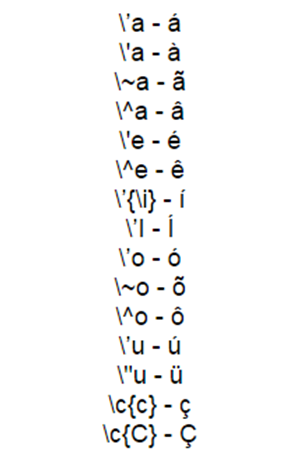
\includegraphics[scale=1.0]{imagens/USPSC-AcentuacaoLaTeX.png} \\
	%Fonte: \citeonline{comandos}
	Fonte: \citefonte{comandos}

\end{figure}

\end{anexosenv}


\end{document}
